\documentclass{beamer}
\usepackage[utf8]{inputenc}
\usepackage[]{amsmath}
\usepackage{graphicx}
\usepackage{physics}
\usepackage{subcaption} % package pour faire des subfigures
\usepackage{multirow} % package pour multirow/multicolumn
\usepackage{booktabs} % package pour top/mid/bottom rule
\usepackage{tcolorbox} % toujours plus de boites
\usepackage{tabularx}
%\usepackage[backend=biber]{biblatex}
%
%
%\addbibresource{Biblio_dbl_quantum.bib}

%\bibliographystyle{stylename}
%\bibliography{Biblio_dbl_quantum}

\title[PhD Defense]{Cross-relaxation in dense ensembles of NV centers and
application to magnetometry}
\author{Clément Pellet-Mary}
\date{PhD Defense}

\usetheme{Malmoe}
\usecolortheme{seahorse}
\setcounter{tocdepth}{1}

%\beamertemplatenavigationsymbolsempty
%\setbeamerfont{page number in head/foot}{size=\large}
%\setbeamertemplate{footline}[frame number]

\expandafter\def\expandafter\insertshorttitle\expandafter{%
  \insertshorttitle\hfill%
  \insertframenumber\,}

\begin{document}
%\begin{frame}
%\maketitle
%\begin{center}
%\includegraphics[width=\textwidth,height=0.5\textheight,keepaspectratio]{logos}
%\end{center}
%\end{frame}

\begin{frame}
\centering
\begin{tcolorbox}[colback=blue!20!white]
\centering
\Large
Cross-relaxation in dense ensembles of NV centers and
application to magnetometry
\end{tcolorbox}
\bigskip
Clément Pellet-Mary PhD Defense
\bigskip
\includegraphics[width=\textwidth,height=0.5\textheight,keepaspectratio]{logos}
\end{frame}

\begin{frame}{Context of my PhD}
\centering
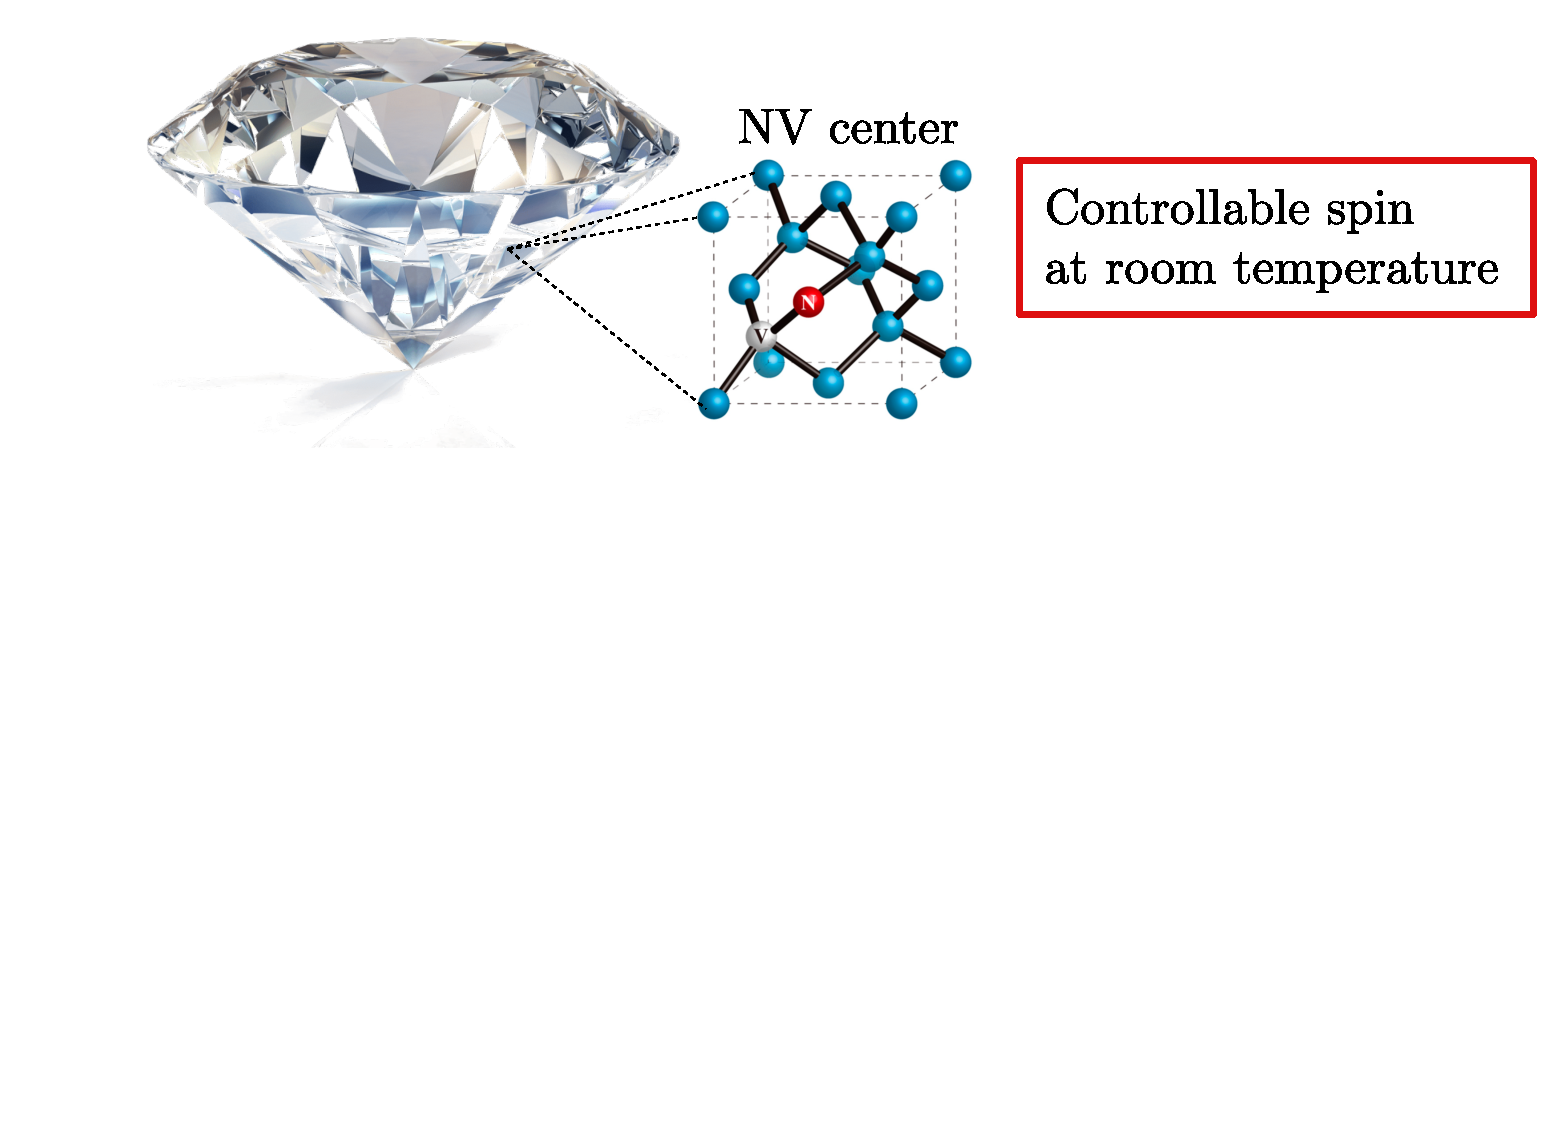
\includegraphics[width=\textwidth,height=0.85\textheight,keepaspectratio]{Slide_contexte_f-4}
\end{frame}

\begin{frame}{Context of my PhD}
\centering
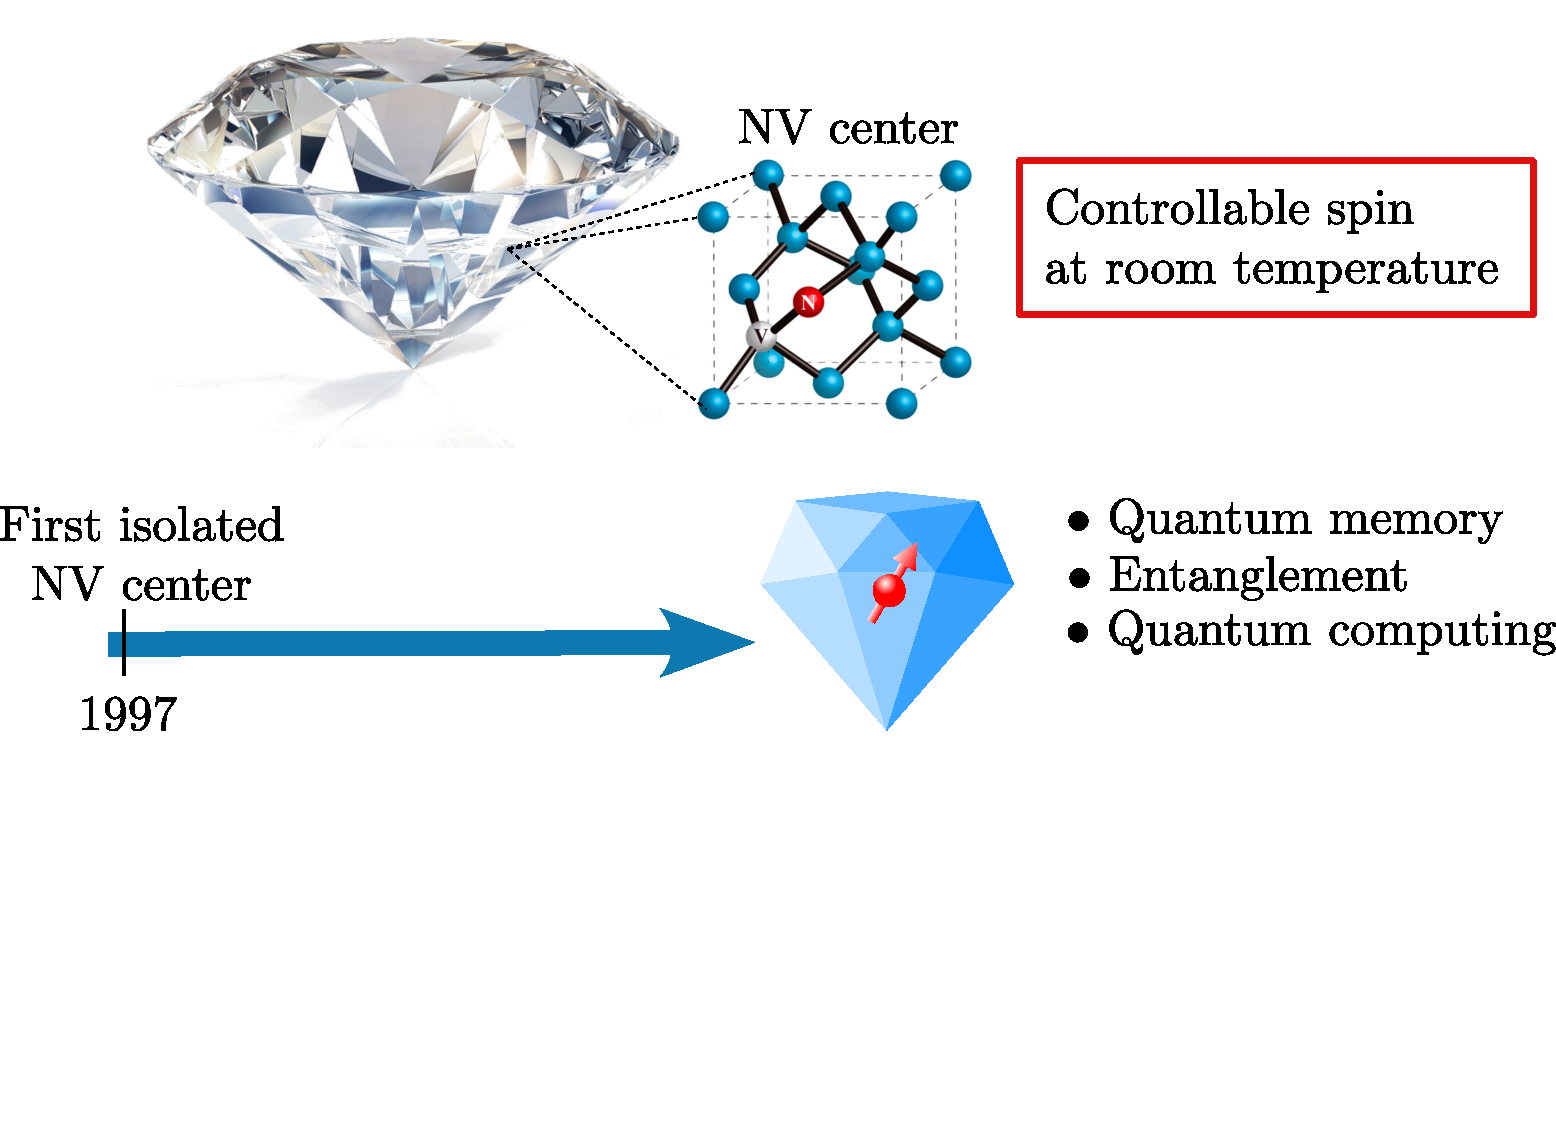
\includegraphics[width=\textwidth,height=0.85\textheight,keepaspectratio]{Slide_contexte_f-3}
\end{frame}

\begin{frame}{Context of my PhD}
\centering
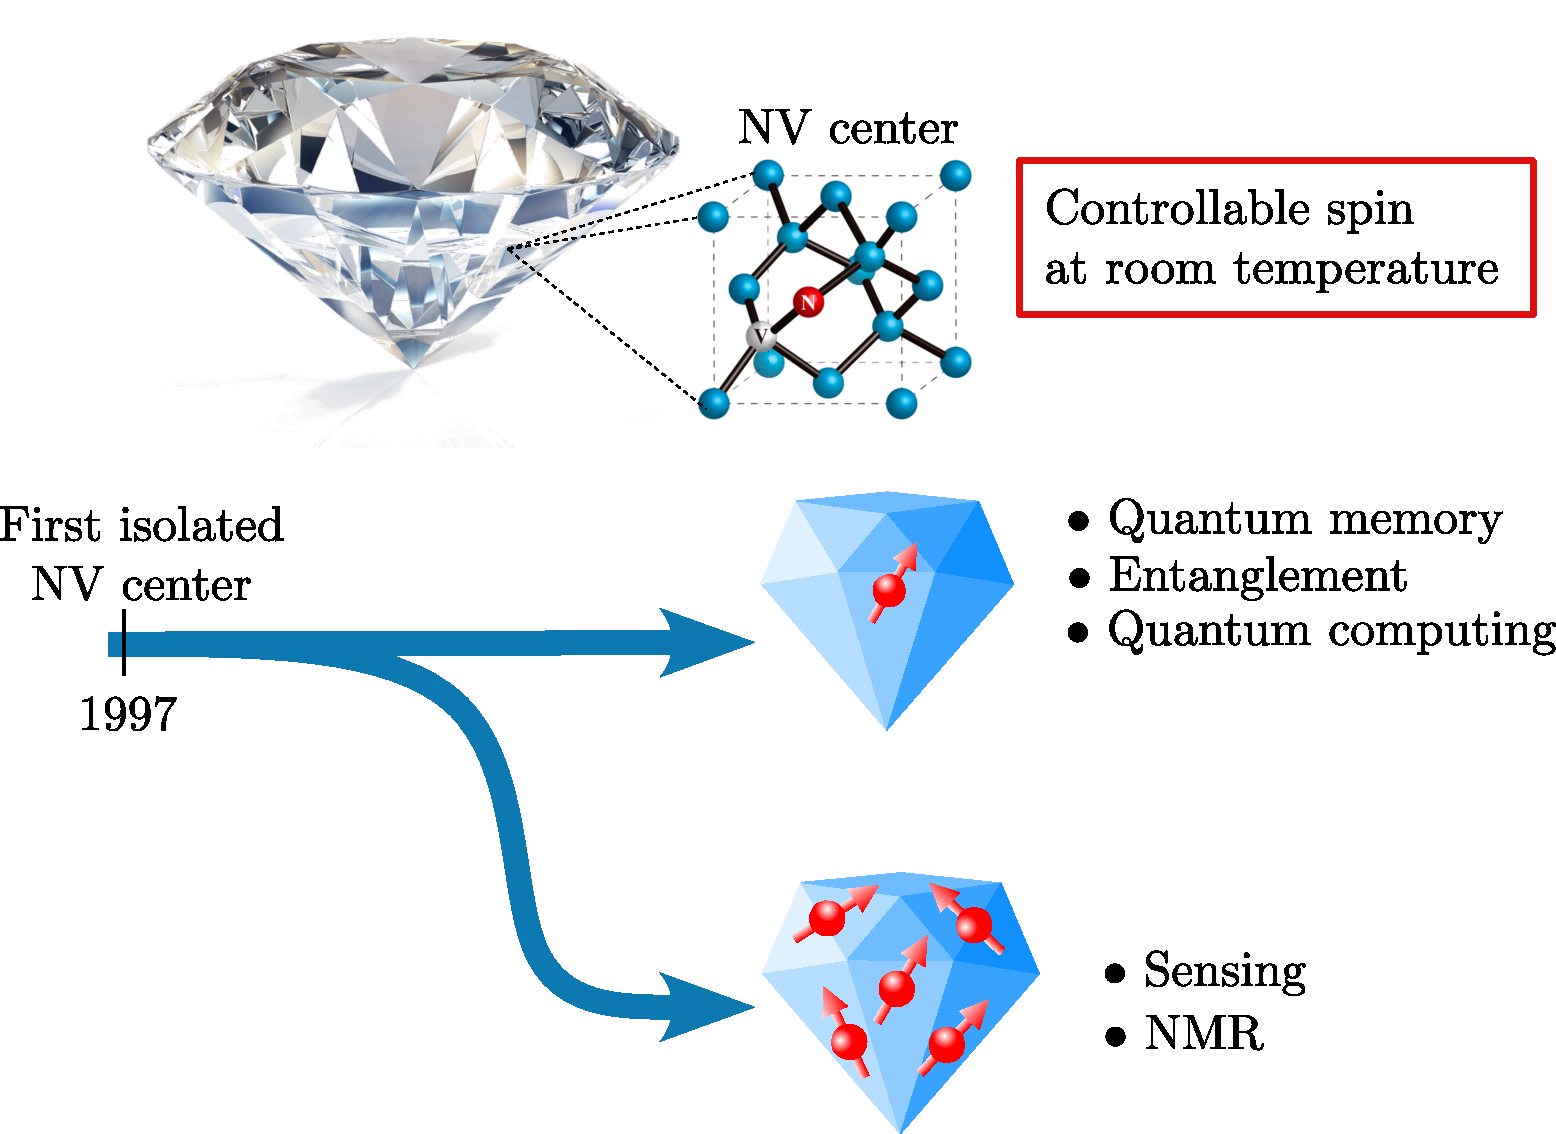
\includegraphics[width=\textwidth,height=0.85\textheight,keepaspectratio]{Slide_contexte_f-2}
\end{frame}

\begin{frame}{Context of my PhD}
\centering
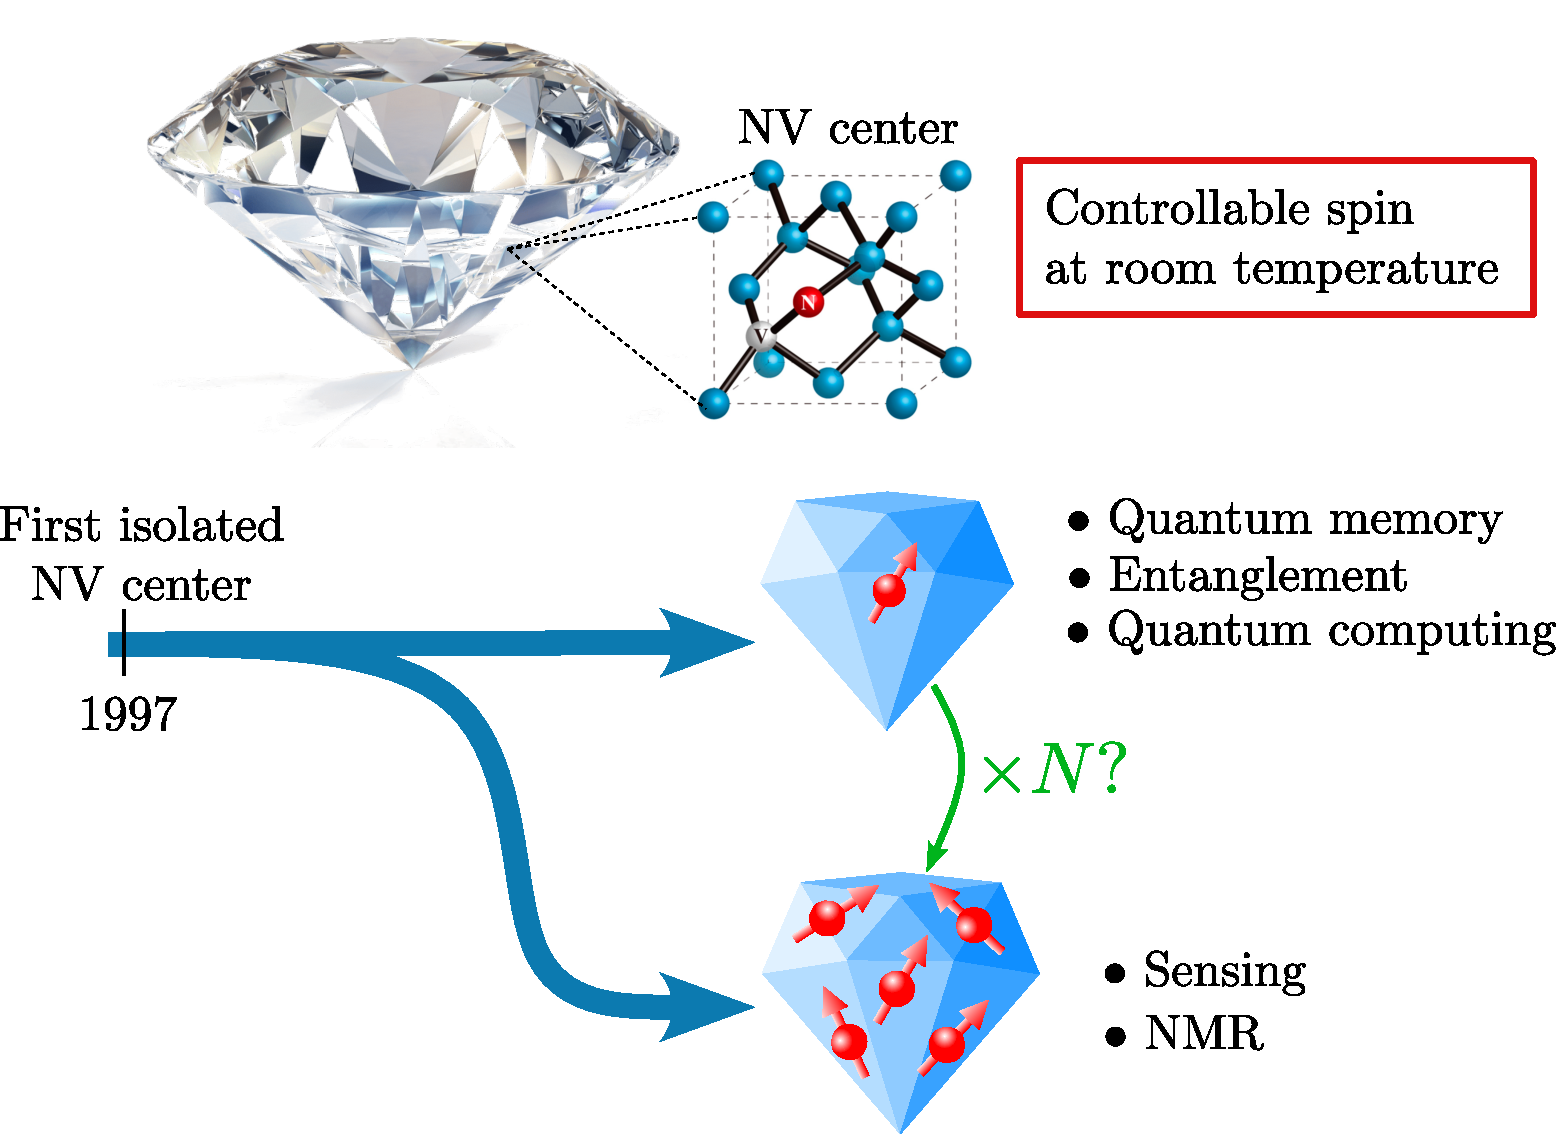
\includegraphics[width=\textwidth,height=0.85\textheight,keepaspectratio]{Slide_contexte_f-1}
\end{frame}

\begin{frame}{Context of my PhD}
\centering
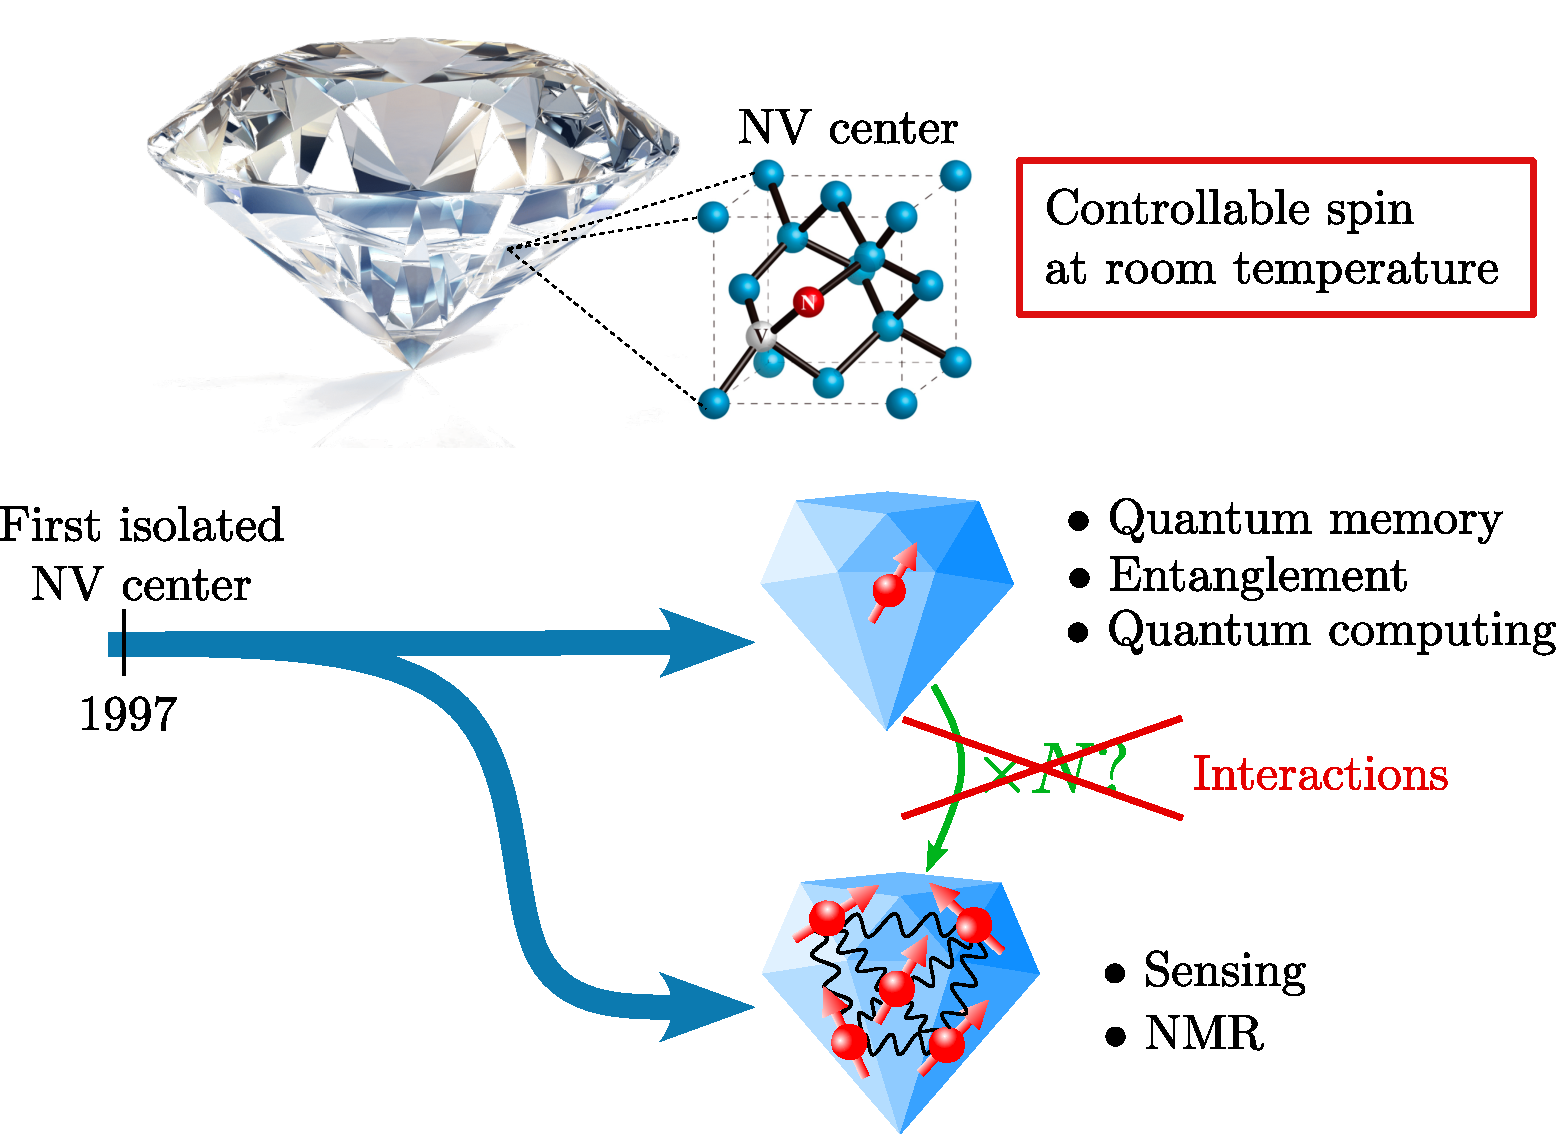
\includegraphics[width=\textwidth,height=0.85\textheight,keepaspectratio]{Slide_contexte_f}
\end{frame}

\begin{frame}{Outline}
\tableofcontents
\end{frame}

\section{Sensing with quantum mechanics}
\begin{frame}{Outline}
\tableofcontents[currentsection]
\end{frame}

\subsection{Quantum sensing}
\begin{frame}{Quantum sensing and metrology}
\centering
\includegraphics[width=\textwidth,height=0.85\textheight,keepaspectratio]{Slide_quantum_metrology}
\end{frame}

\subsection{Magnetometry}
\begin{frame}{Key properties of magnetometers}
\centering
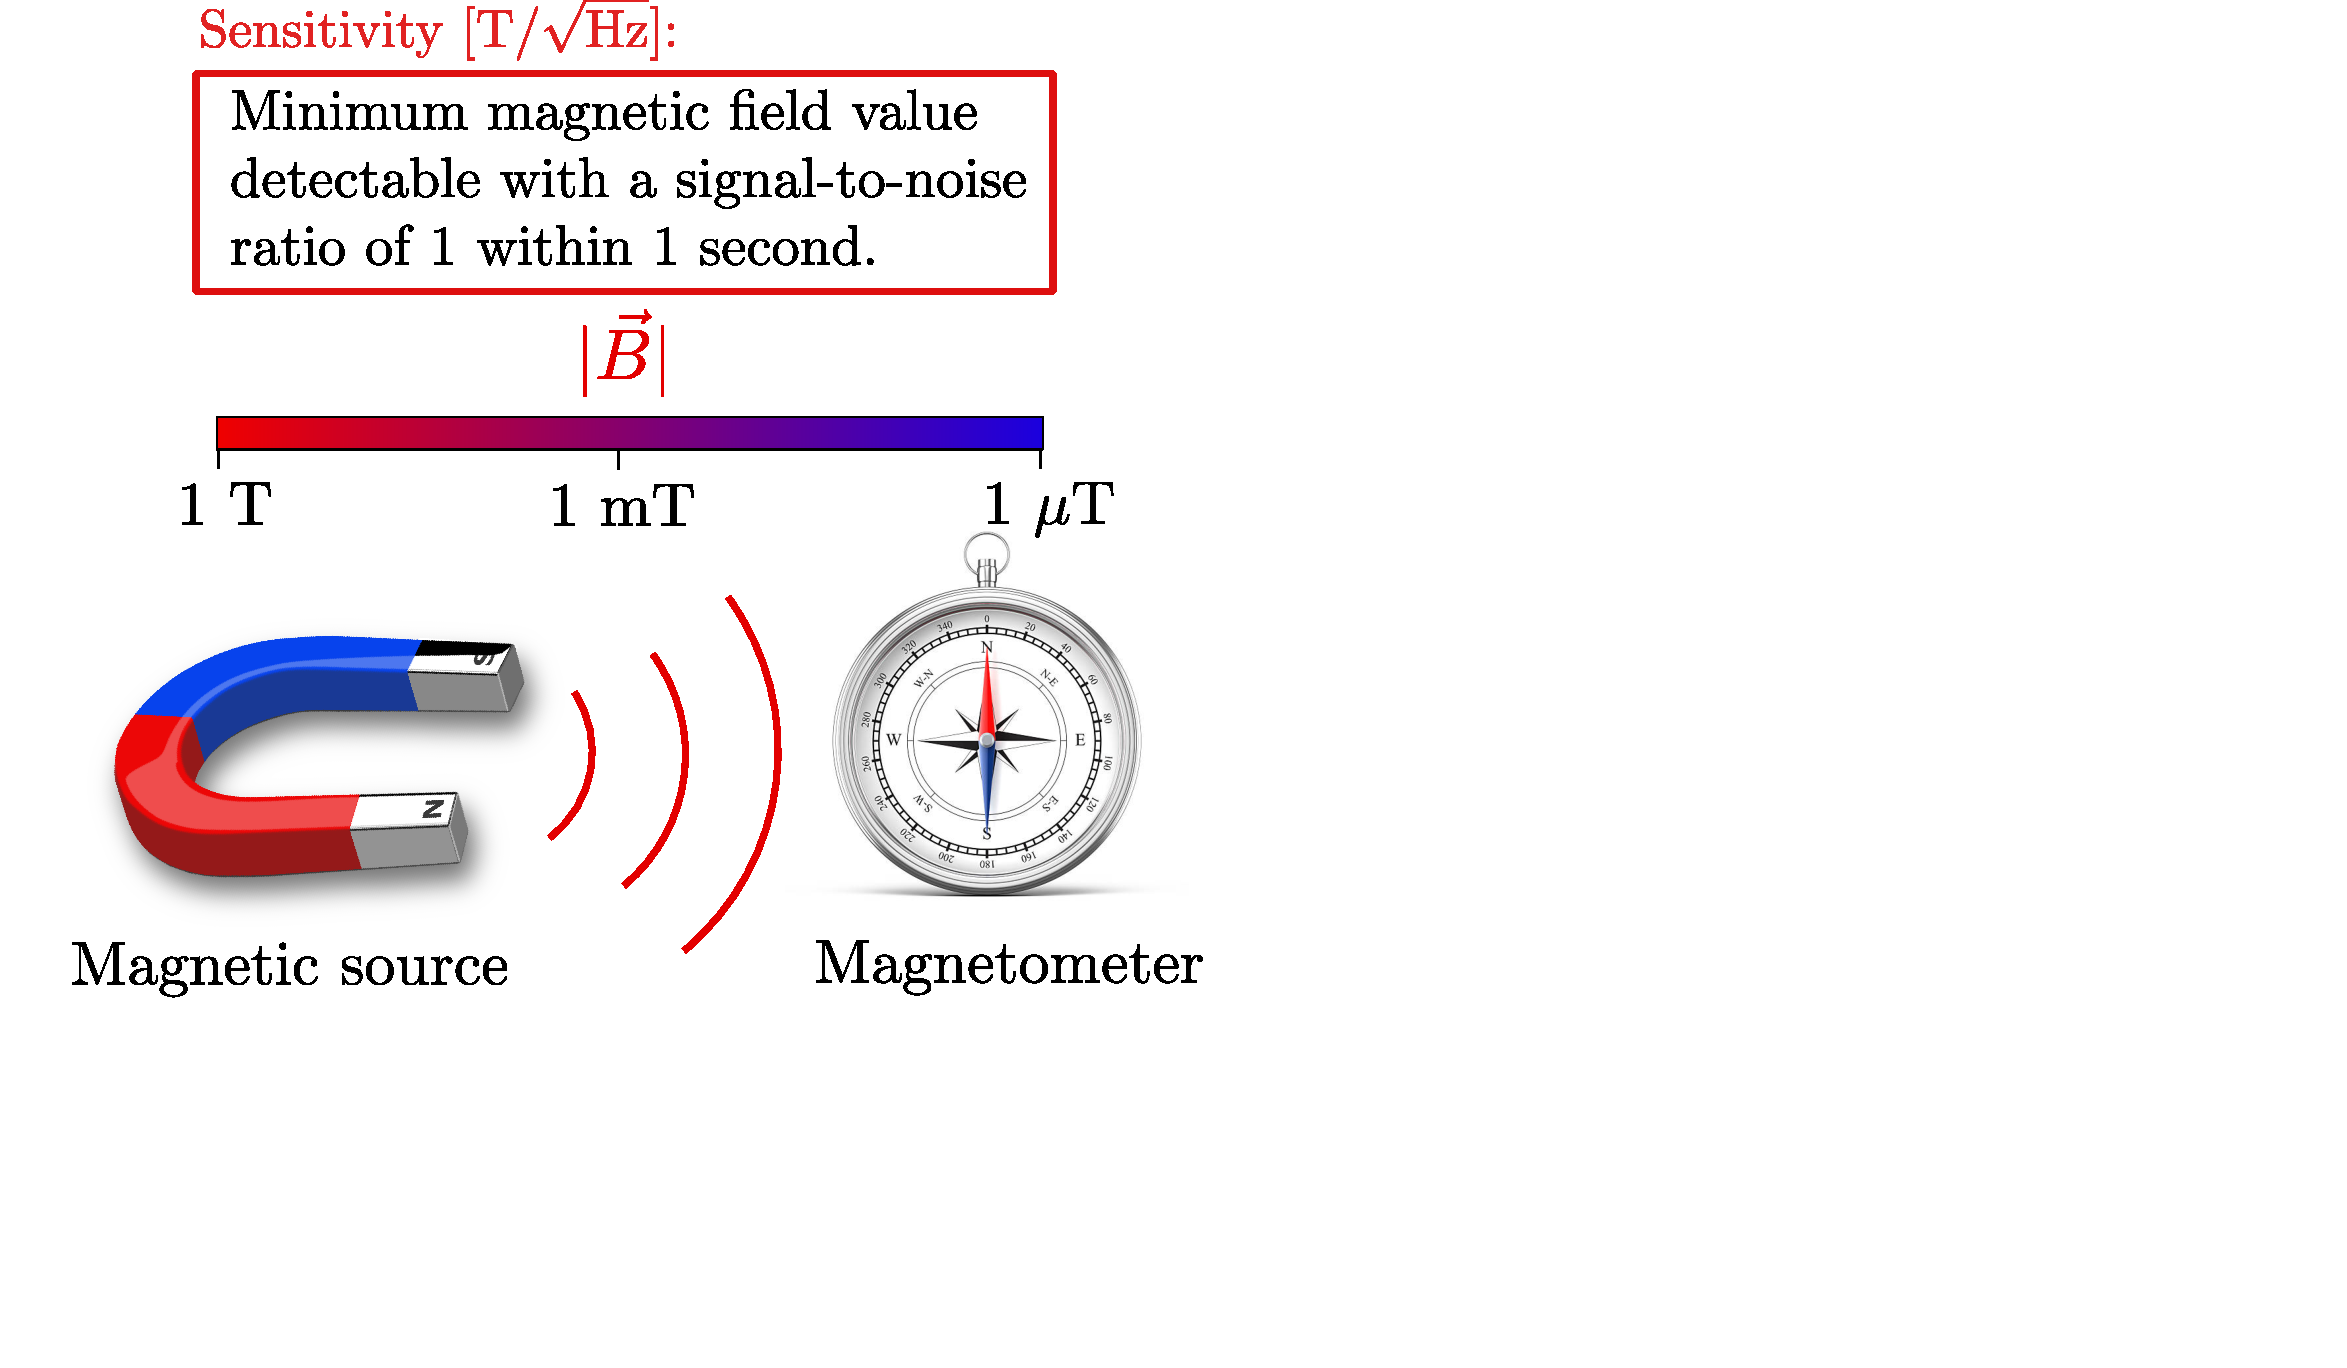
\includegraphics[width=\textwidth,height=0.85\textheight,keepaspectratio]{Slide_magnetometer_size_f-2}
\end{frame}

\begin{frame}{Key properties of magnetometers}
\centering
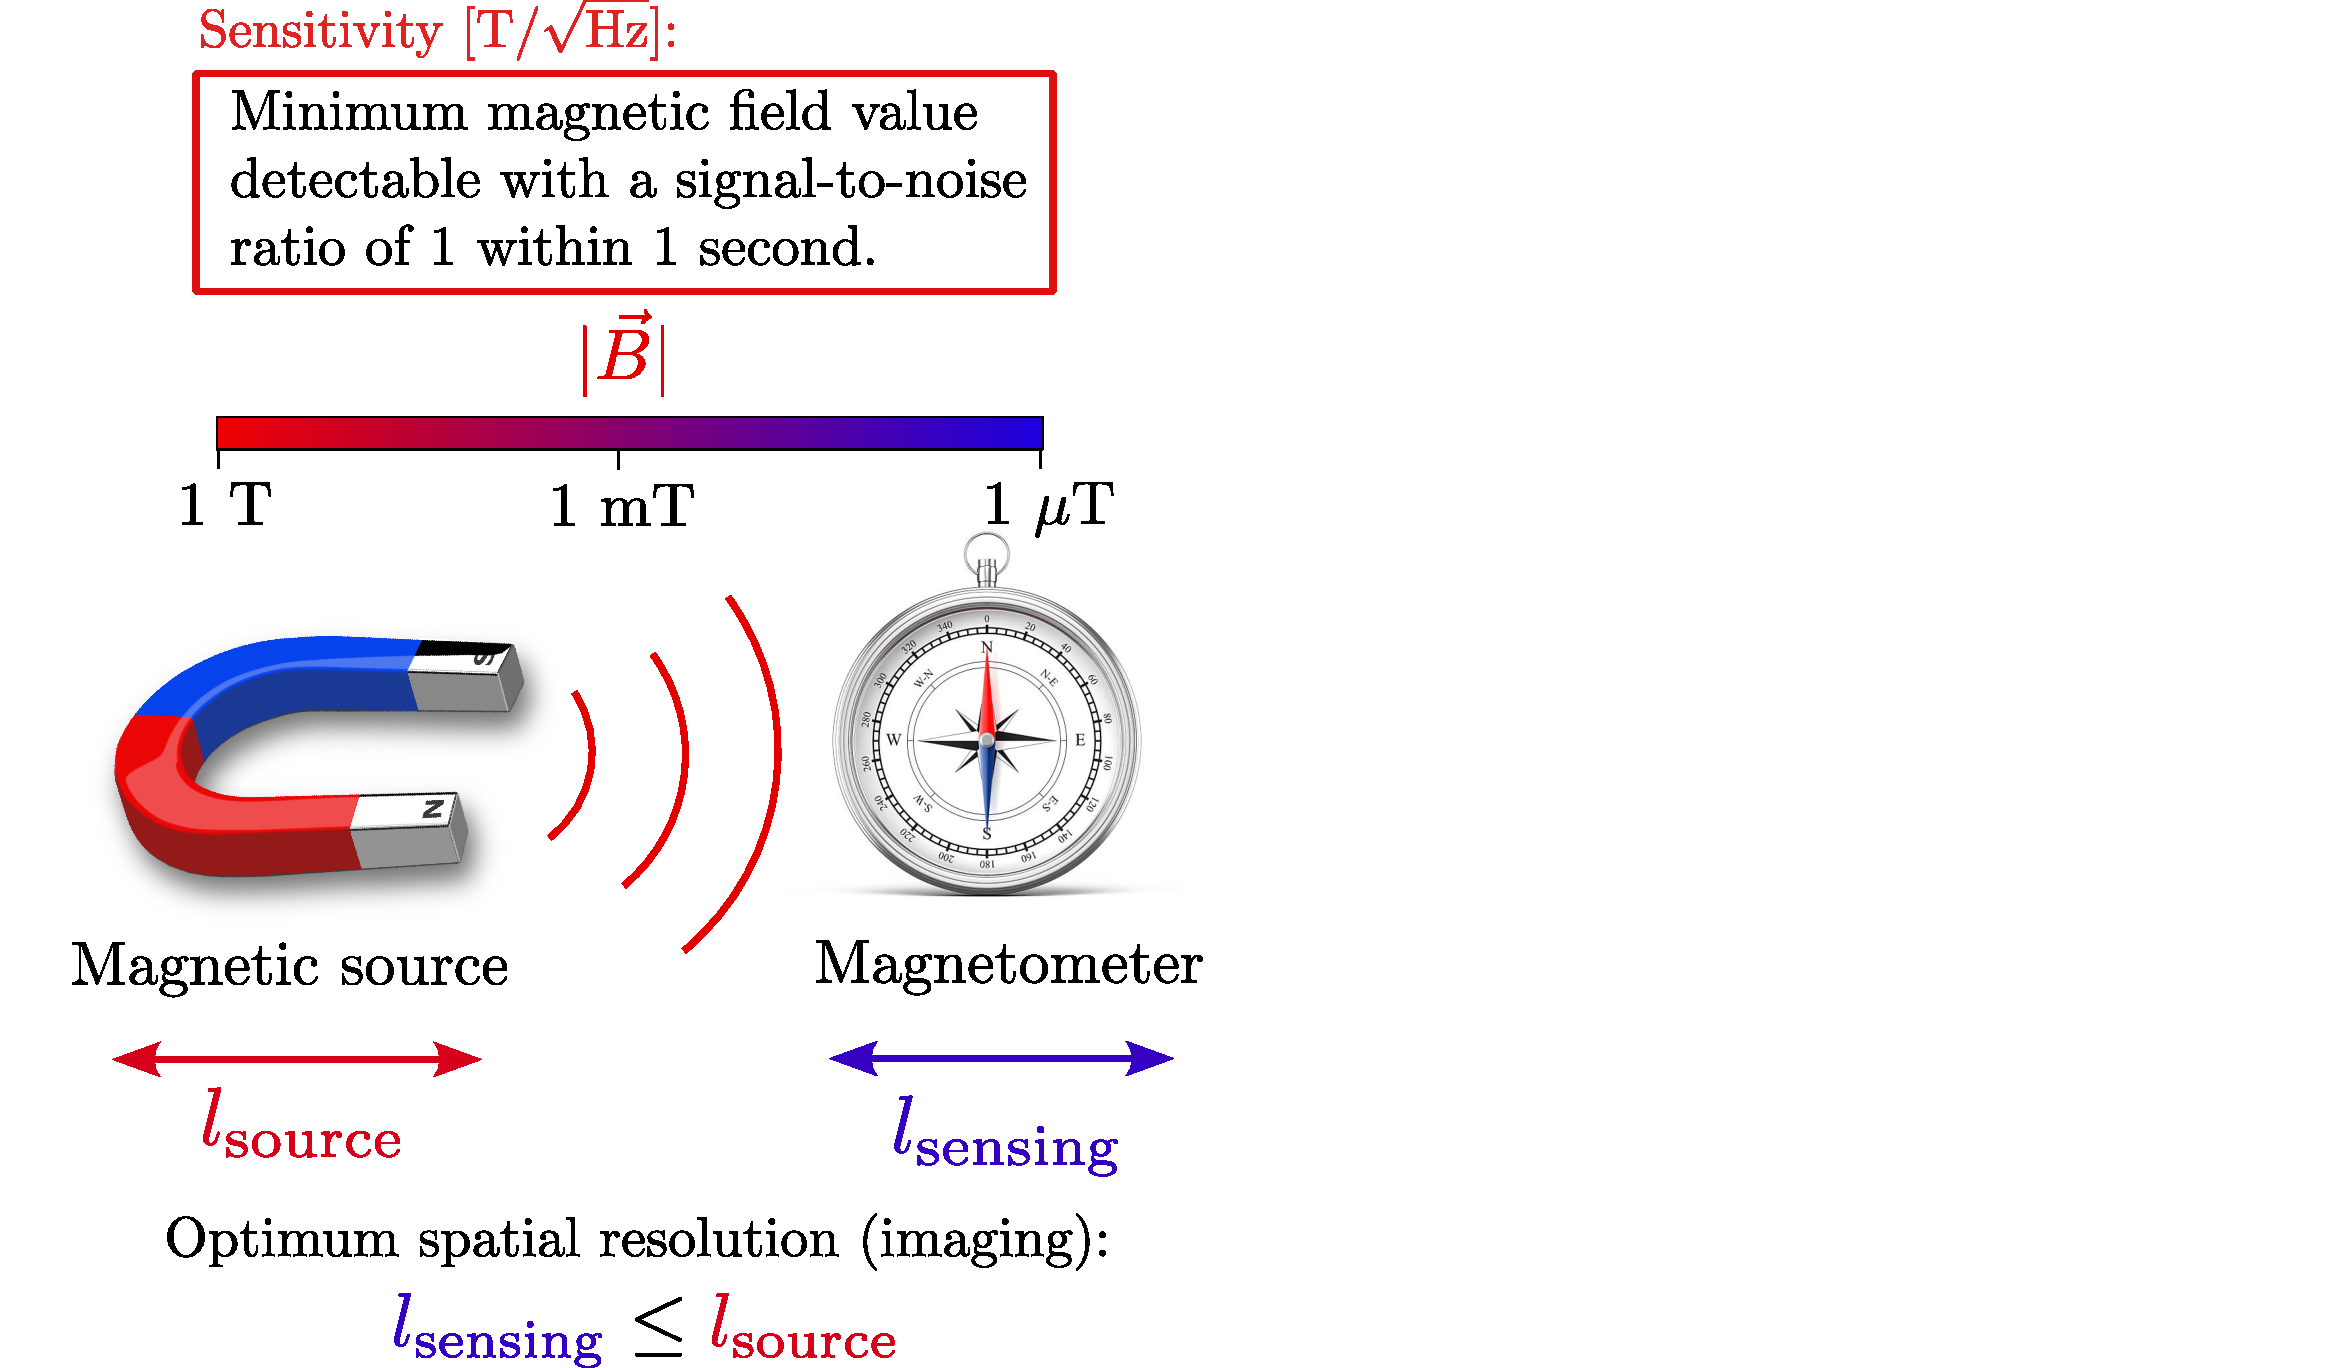
\includegraphics[width=\textwidth,height=0.85\textheight,keepaspectratio]{Slide_magnetometer_size_f-1}
\end{frame}

\begin{frame}{Key properties of magnetometers}
\centering
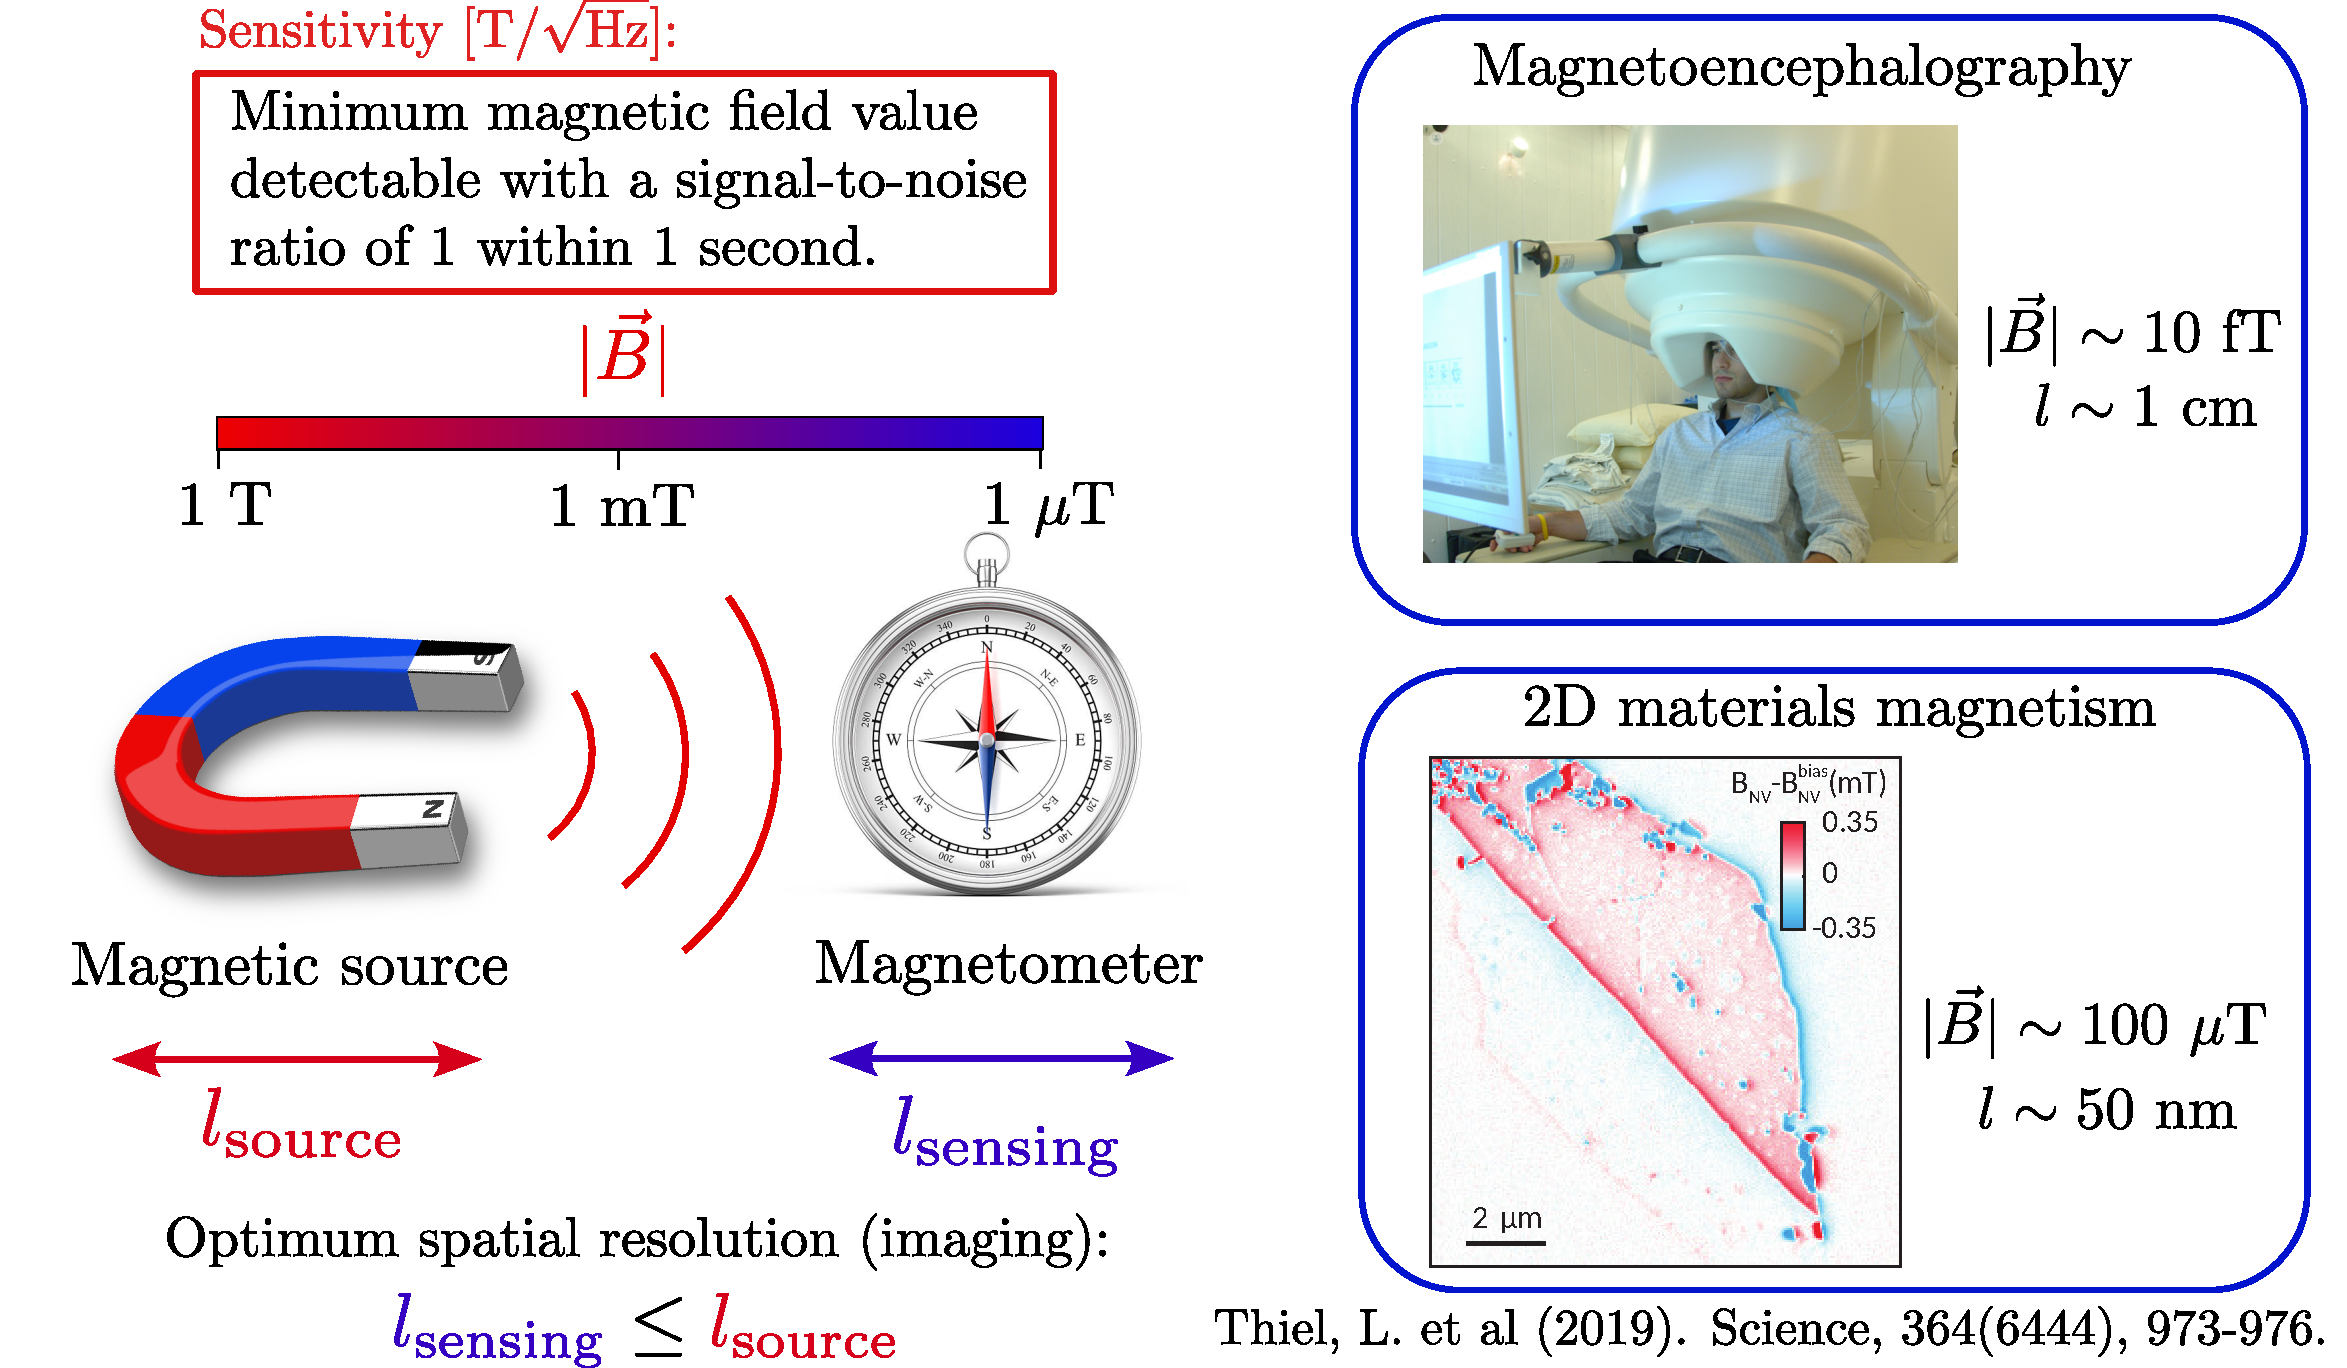
\includegraphics[width=\textwidth,height=0.85\textheight,keepaspectratio]{Slide_magnetometer_size_f}
\end{frame}

\begin{frame}{Sate of the art magnetometers}
\centering
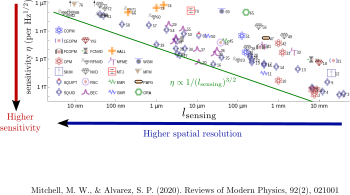
\includegraphics[width=\textwidth,height=0.85\textheight,keepaspectratio]{Slide_quantum_magnetometers_bare_1}
\end{frame}

\begin{frame}{Sate of the art magnetometers}
\centering
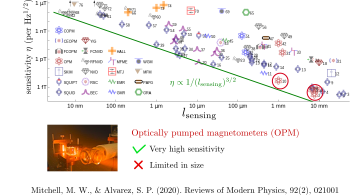
\includegraphics[width=\textwidth,height=0.85\textheight,keepaspectratio]{Slide_quantum_magnetometers_OPM}
\end{frame}

\begin{frame}{State of the art magnetometers}
\centering
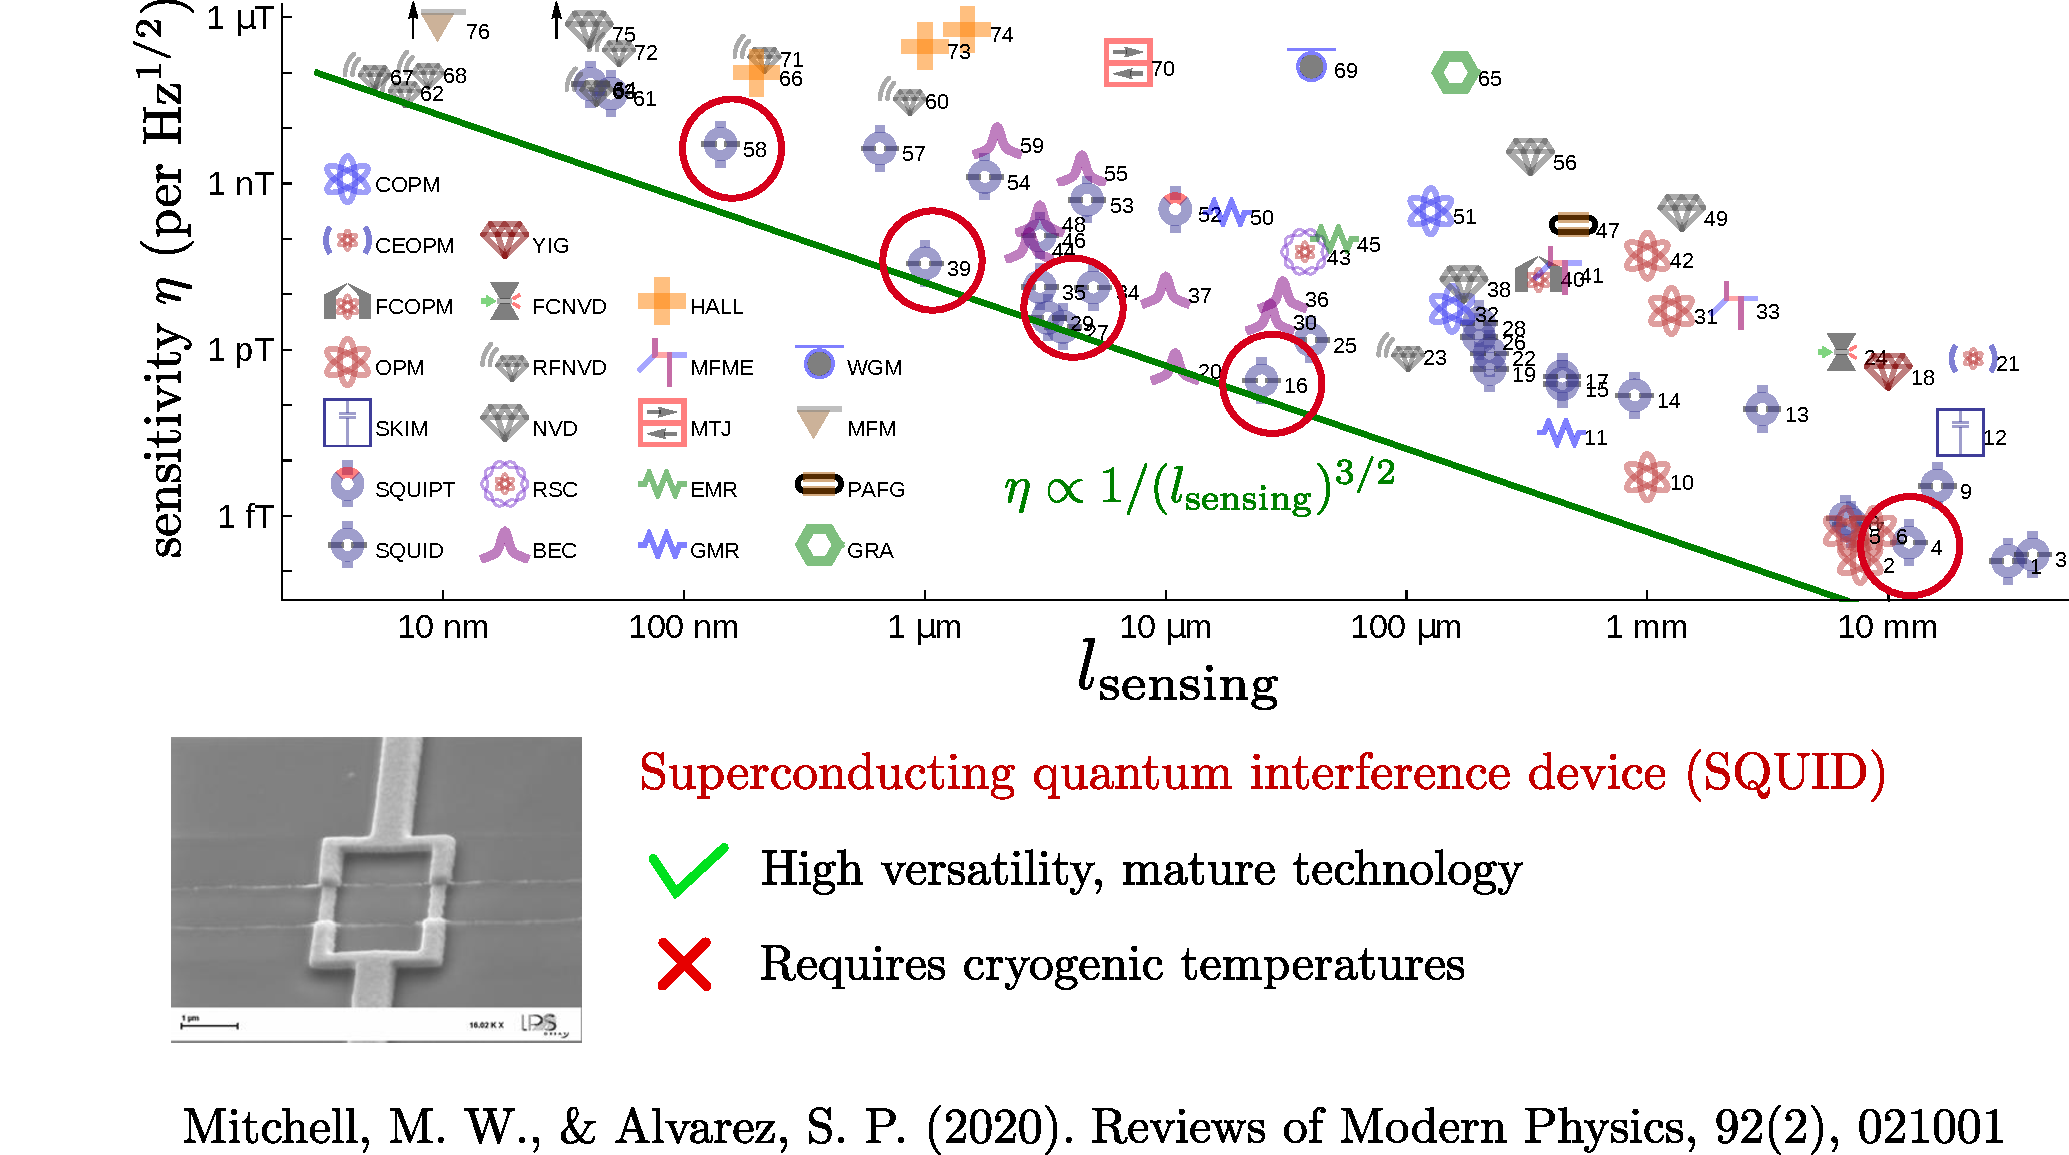
\includegraphics[width=\textwidth,height=0.85\textheight,keepaspectratio]{Slide_quantum_magnetometers_SQUID}
\end{frame}

\begin{frame}{State of the art magnetometers}
\centering
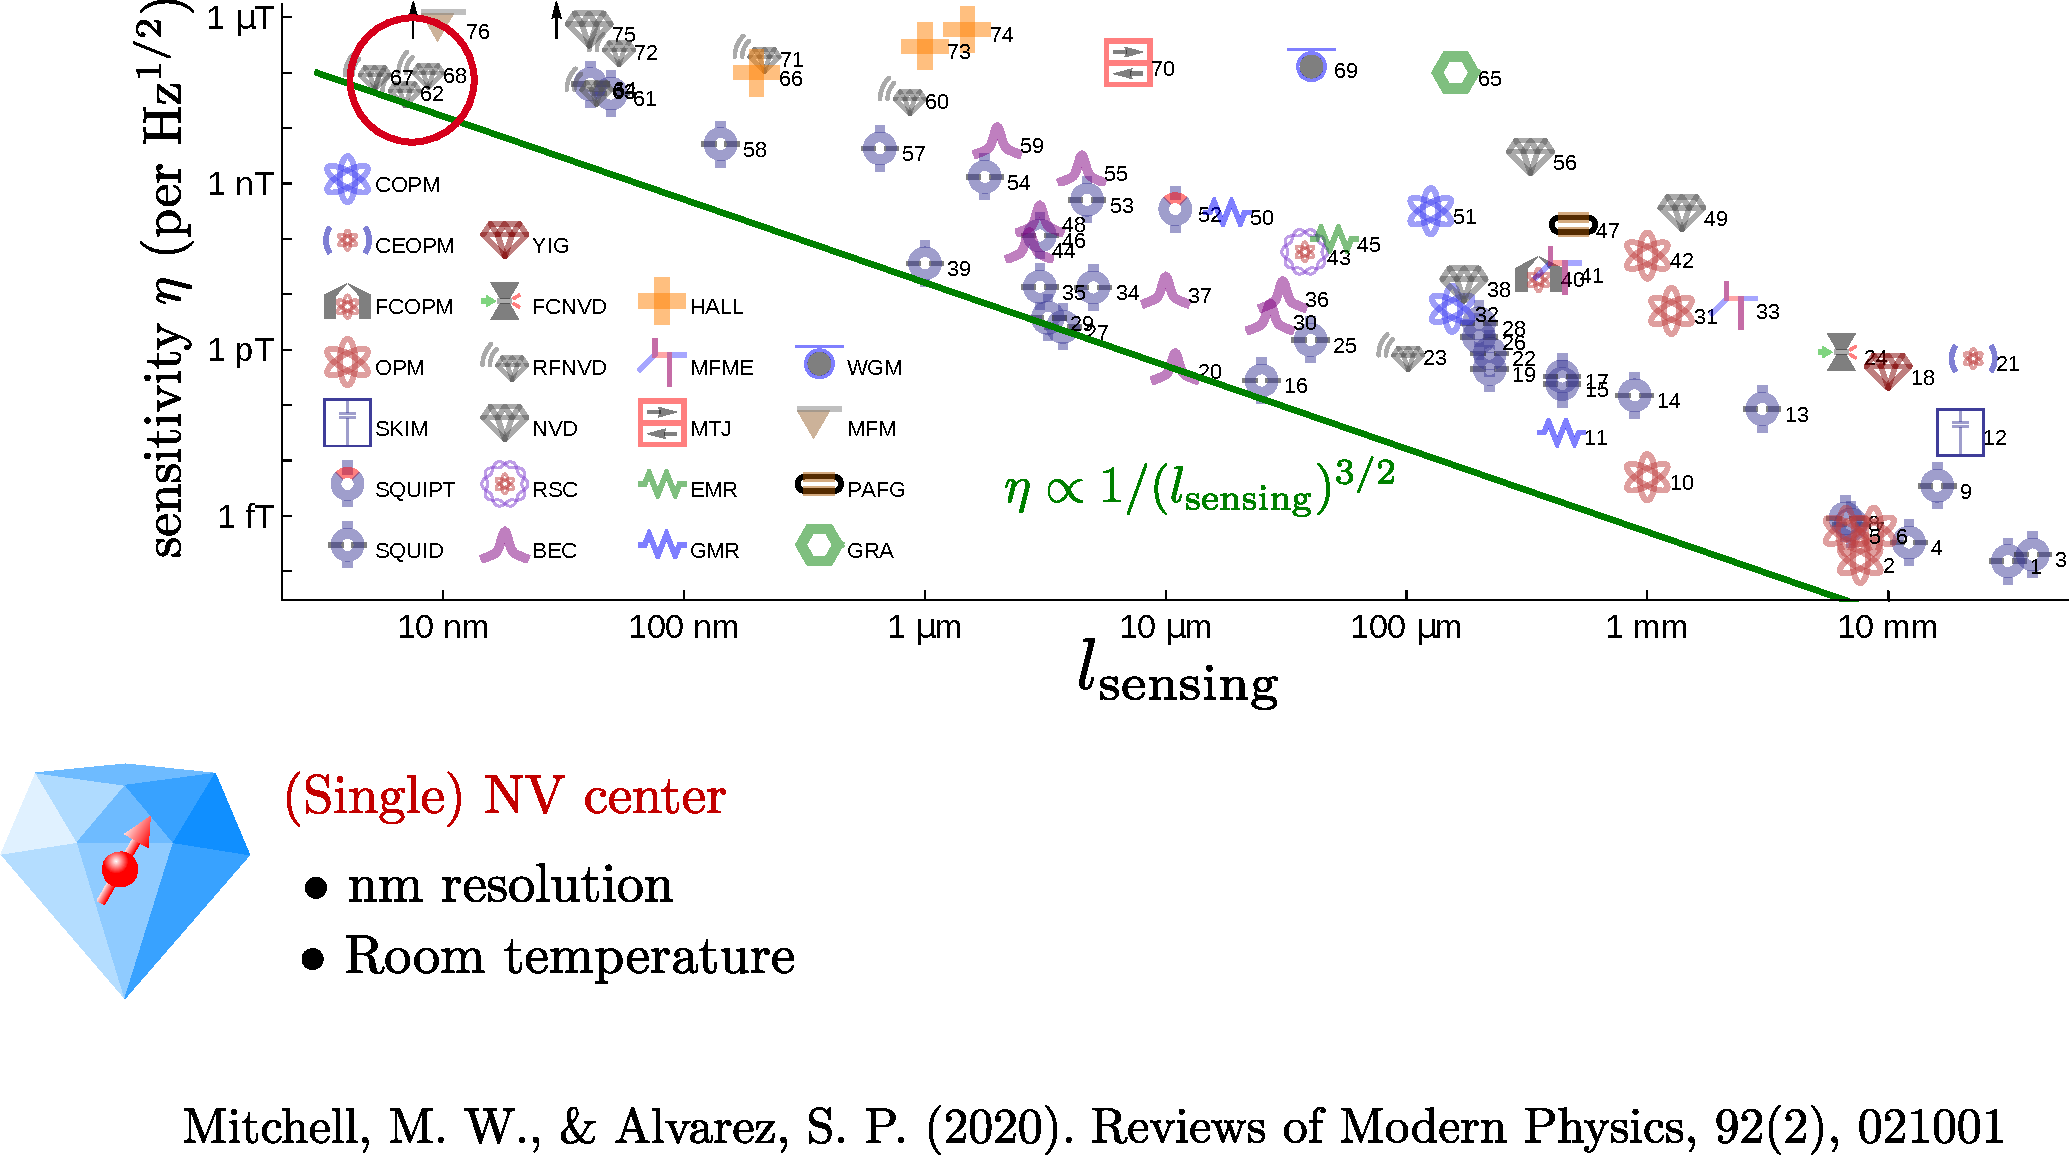
\includegraphics[width=\textwidth,height=0.85\textheight,keepaspectratio]{Slide_quantum_magnetometers_NV_n-3}
\end{frame}

\begin{frame}{State of the art magnetometers}
\centering
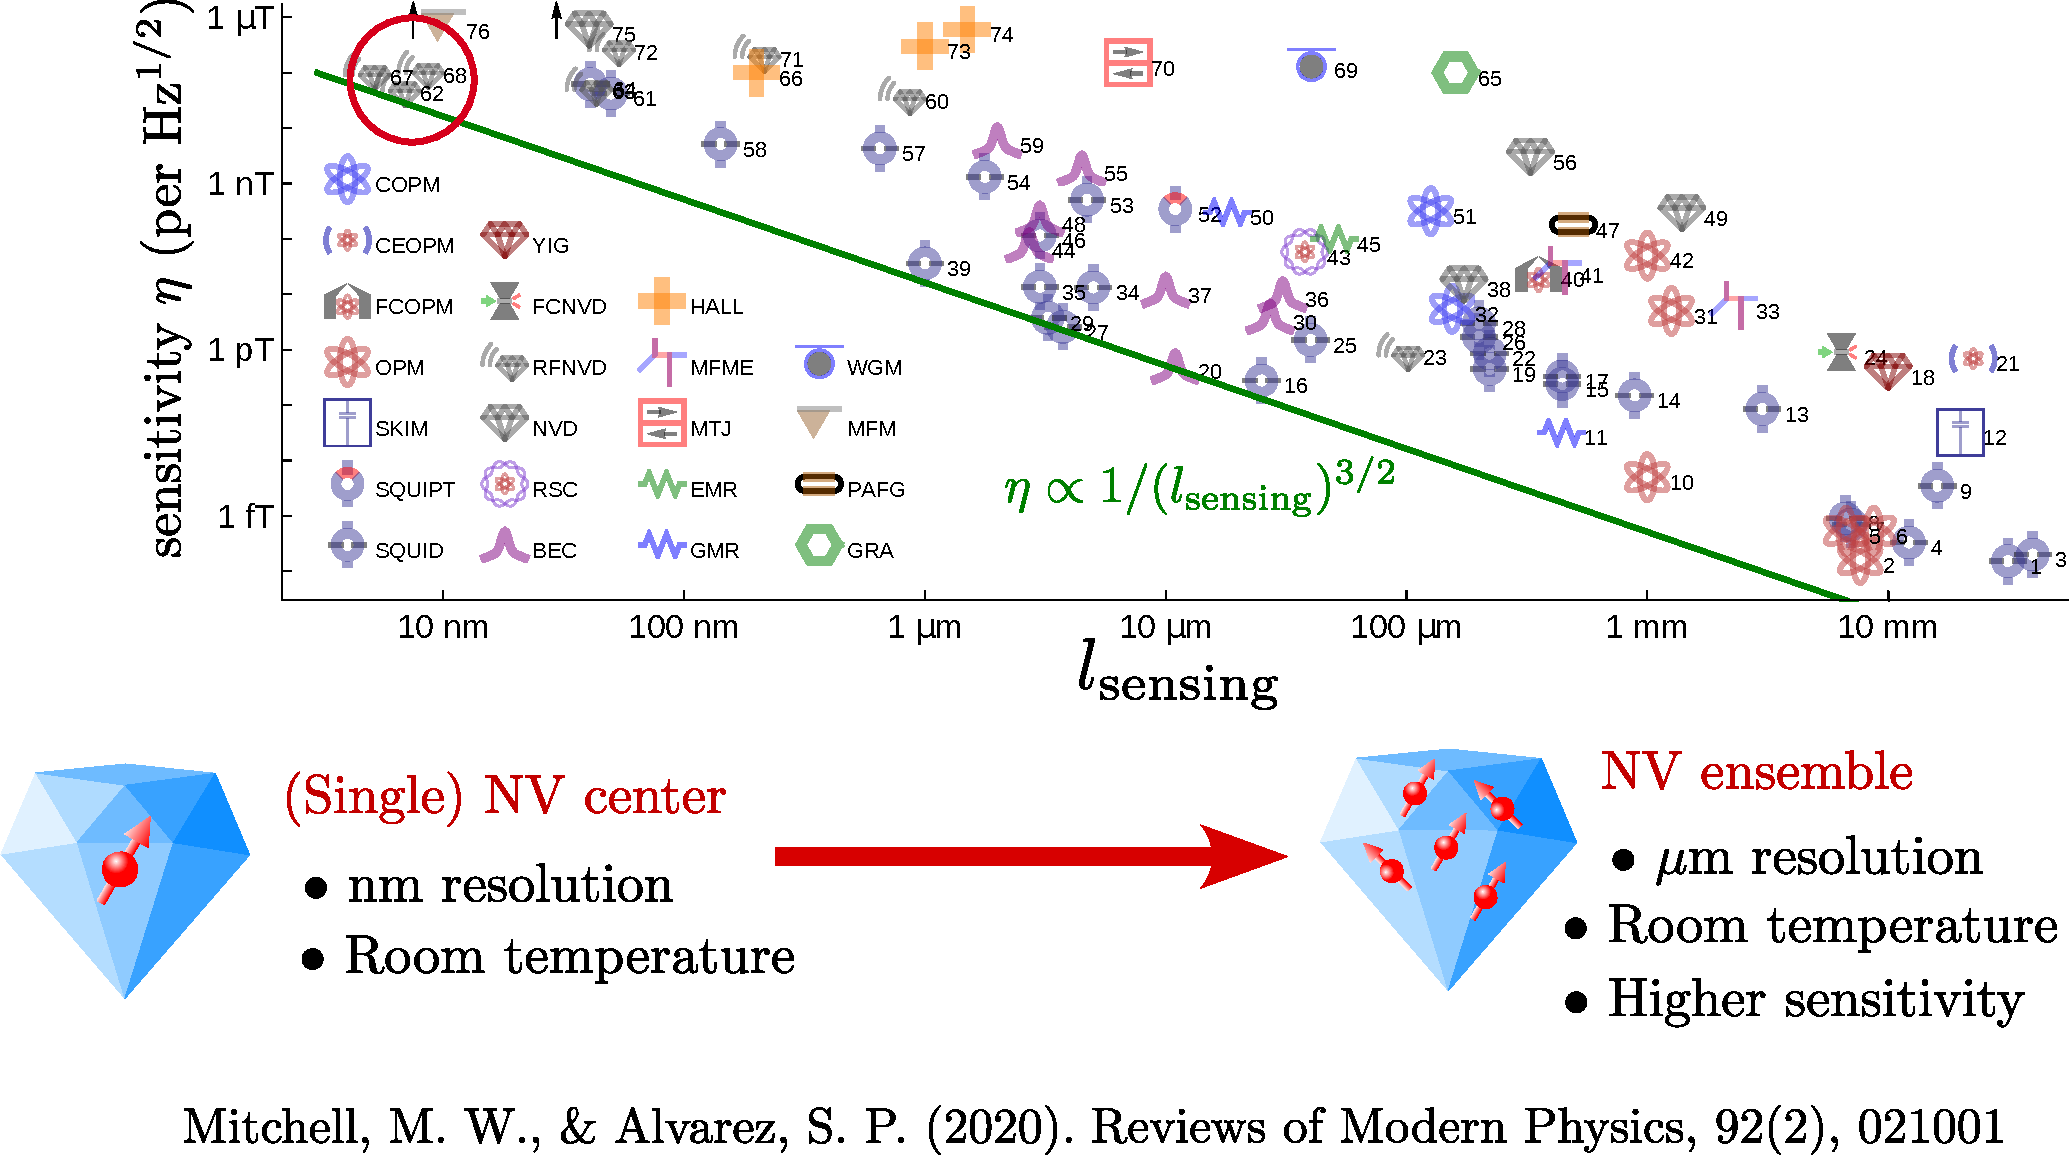
\includegraphics[width=\textwidth,height=0.85\textheight,keepaspectratio]{Slide_quantum_magnetometers_NV_n-2}
\end{frame}

\begin{frame}{State of the art magnetometers}
\centering
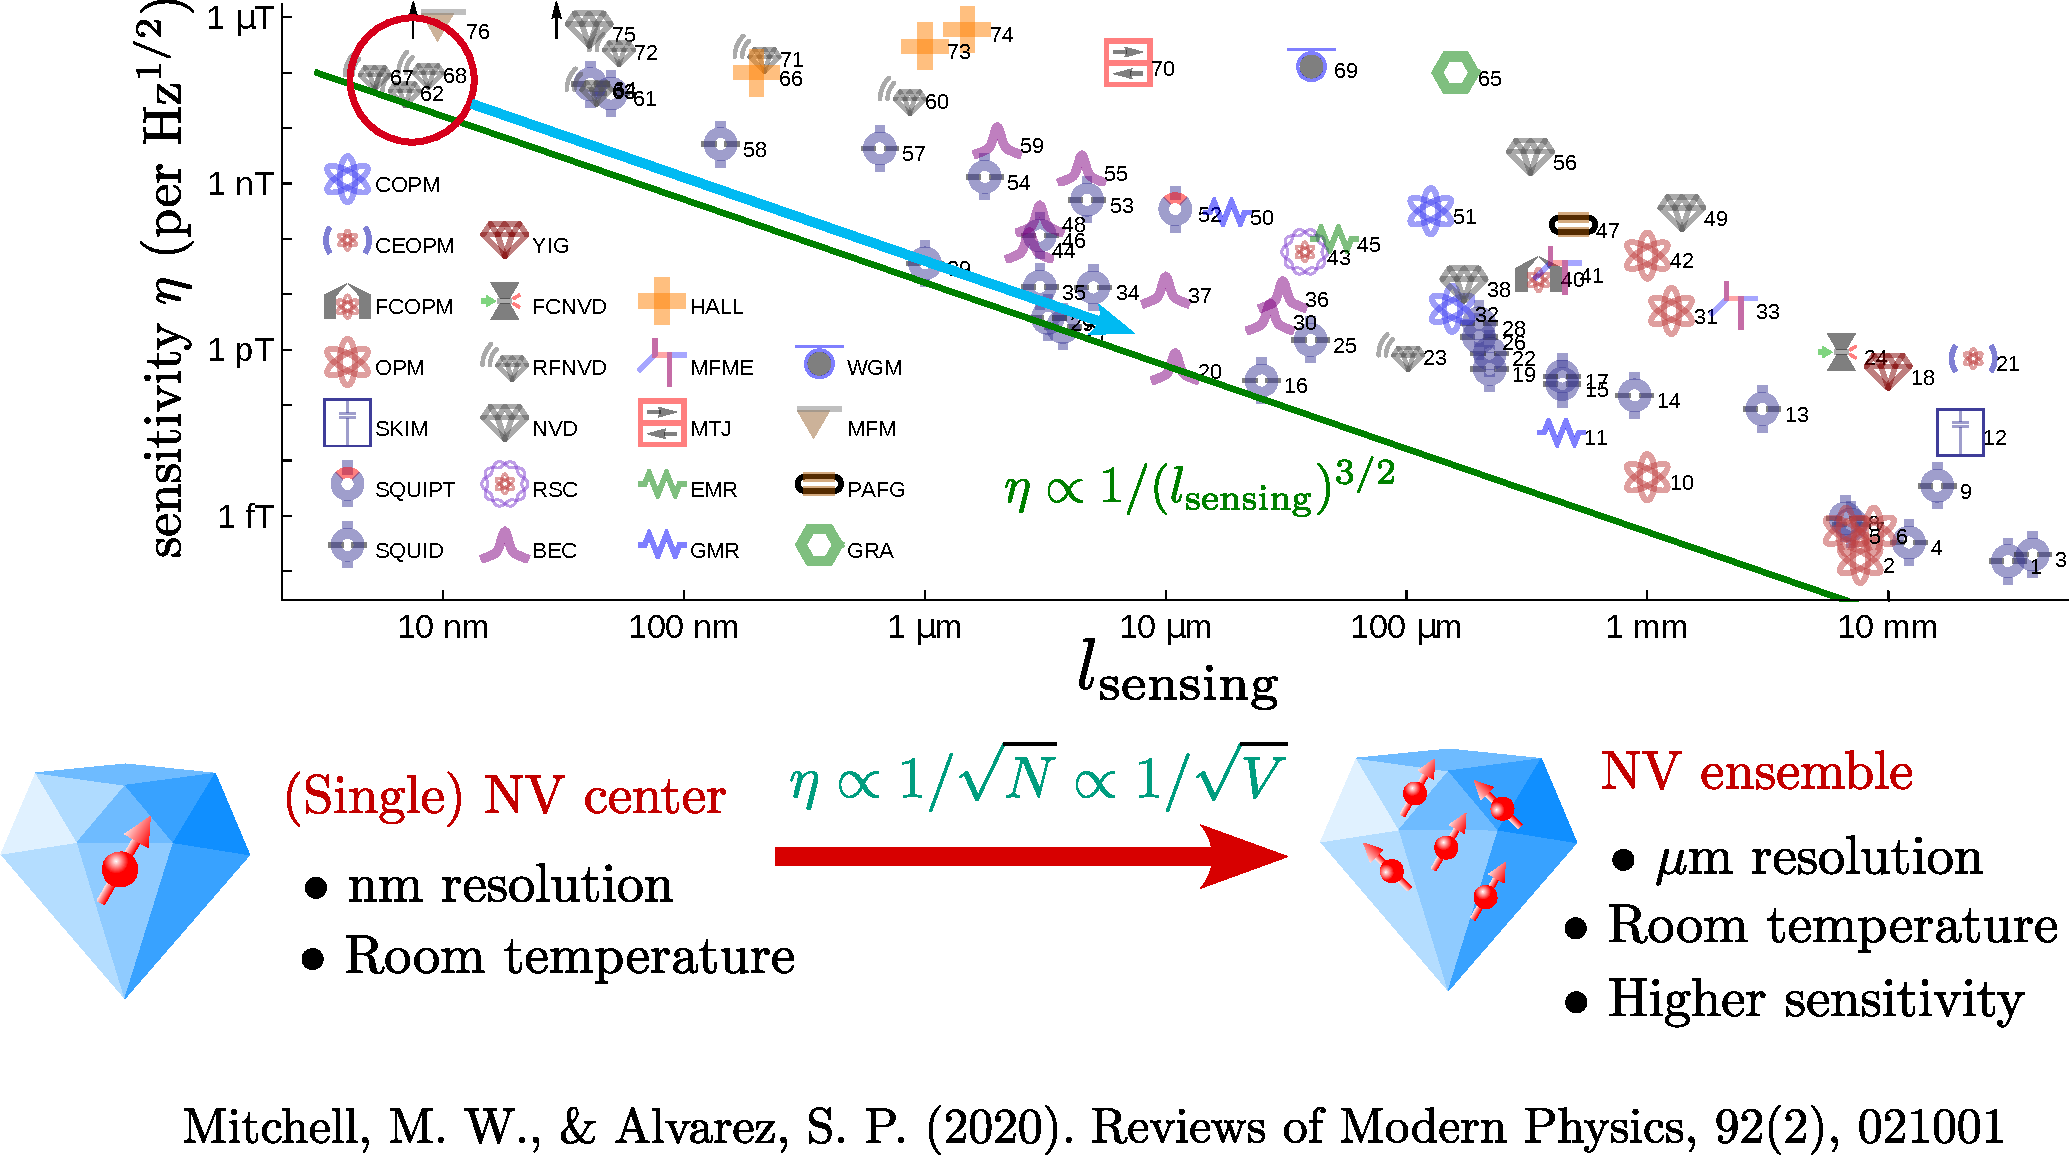
\includegraphics[width=\textwidth,height=0.85\textheight,keepaspectratio]{Slide_quantum_magnetometers_NV_n-1}
\end{frame}

\begin{frame}{State of the art magnetometers}
\centering
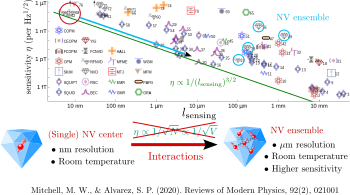
\includegraphics[width=\textwidth,height=0.85\textheight,keepaspectratio]{Slide_quantum_magnetometers_NV_n}
\end{frame}

\begin{frame}{State of the art magnetometers}
\centering
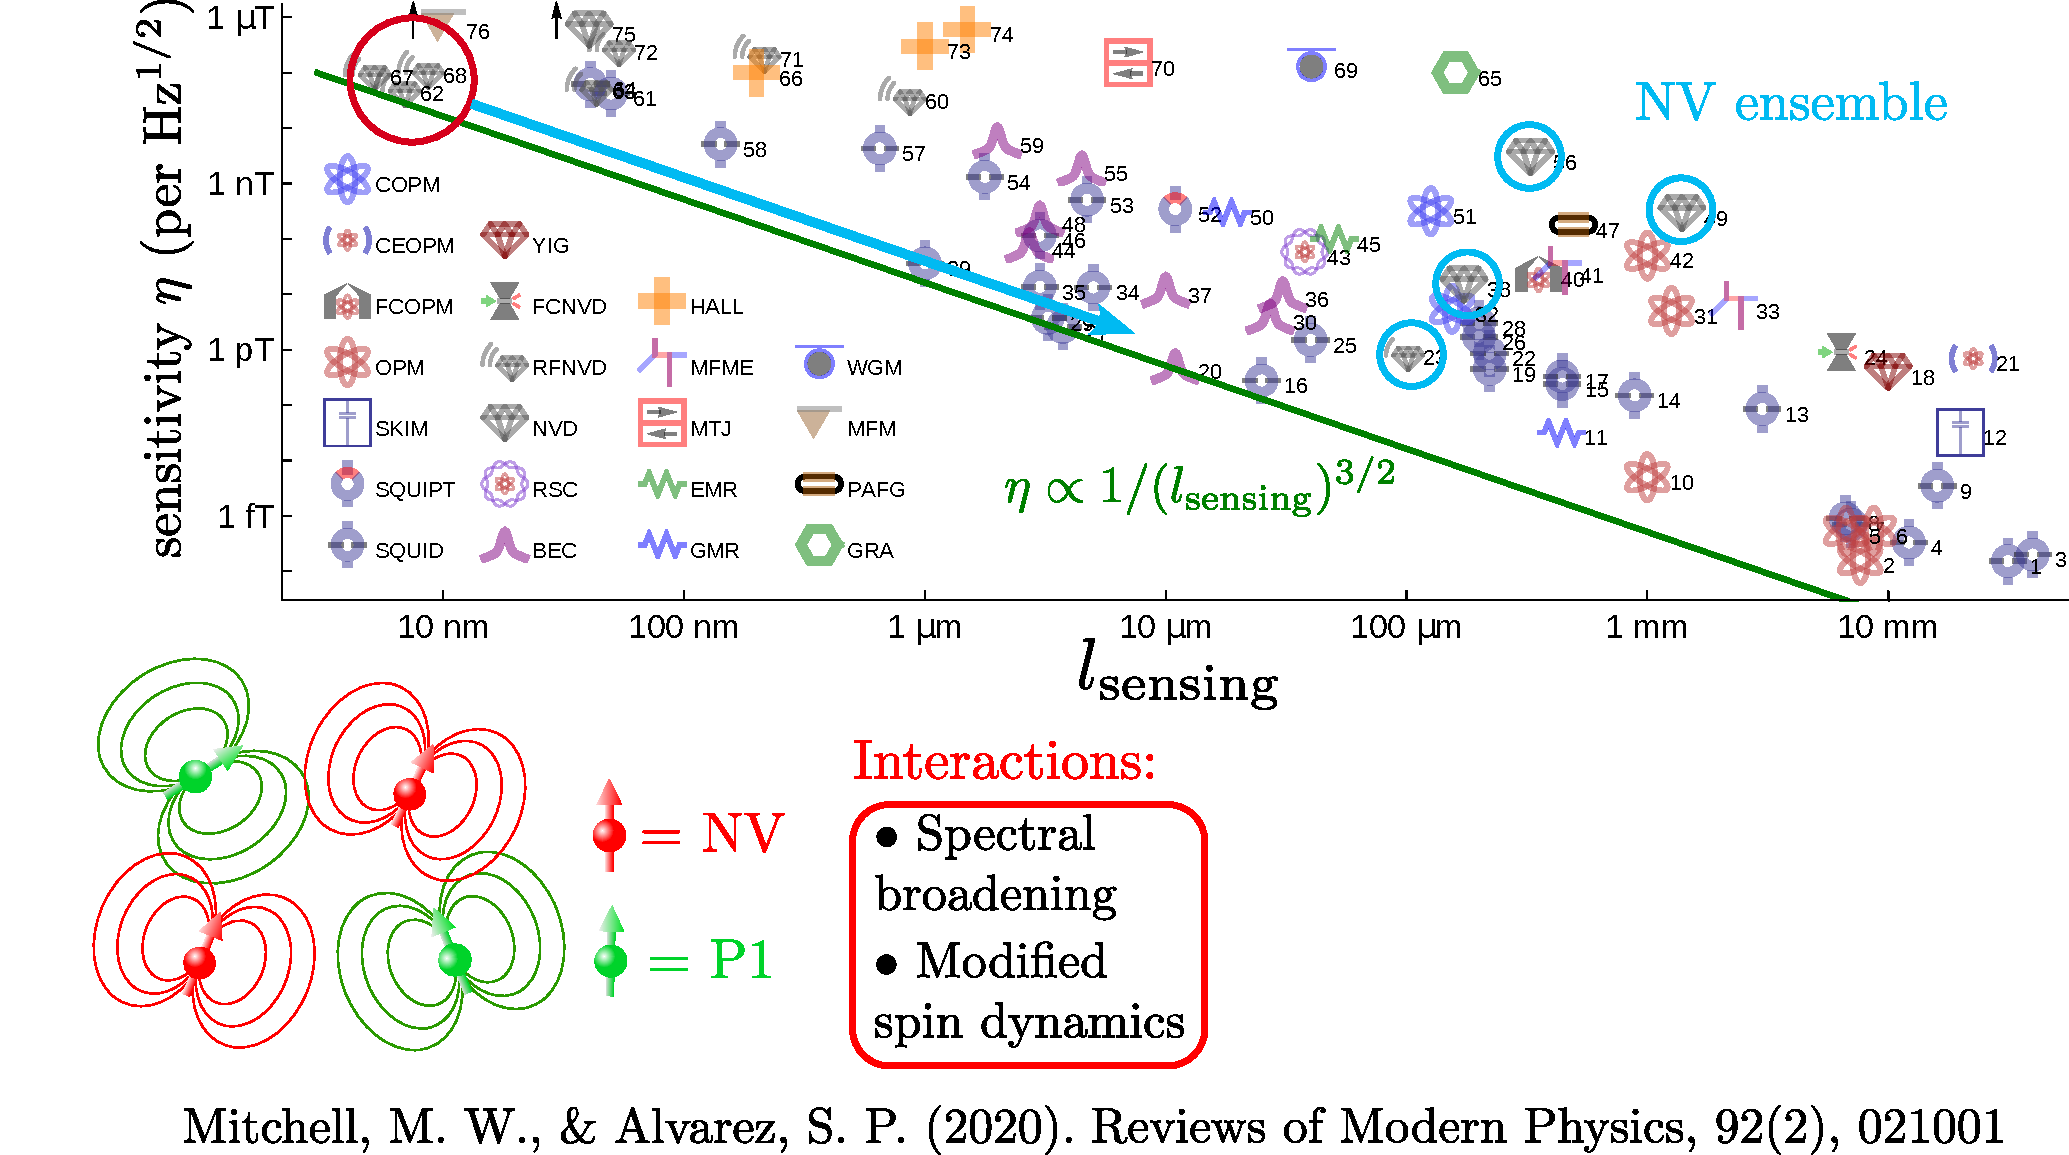
\includegraphics[width=\textwidth,height=0.85\textheight,keepaspectratio]{Slide_quantum_magnetometers_NV_n+1}
\end{frame}

\begin{frame}{State of the art magnetometers}
\centering
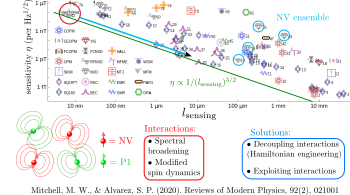
\includegraphics[width=\textwidth,height=0.85\textheight,keepaspectratio]{Slide_quantum_magnetometers_NV_n+2}
\end{frame}


%\begin{frame}{NV center overview}
%\centering
%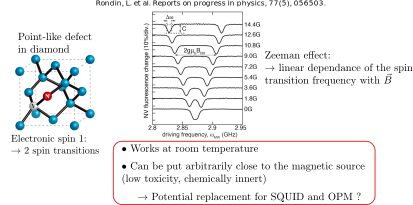
\includegraphics[width=\textwidth,height=0.85\textheight,keepaspectratio]{Slide_NV_rapido}
%\end{frame}


\section{NV center spin properties}
\subsection{Diamond properties}
\begin{frame}{Outline}
\tableofcontents[currentsection]
\end{frame}

\begin{frame}{Colored centers in diamond}
\centering
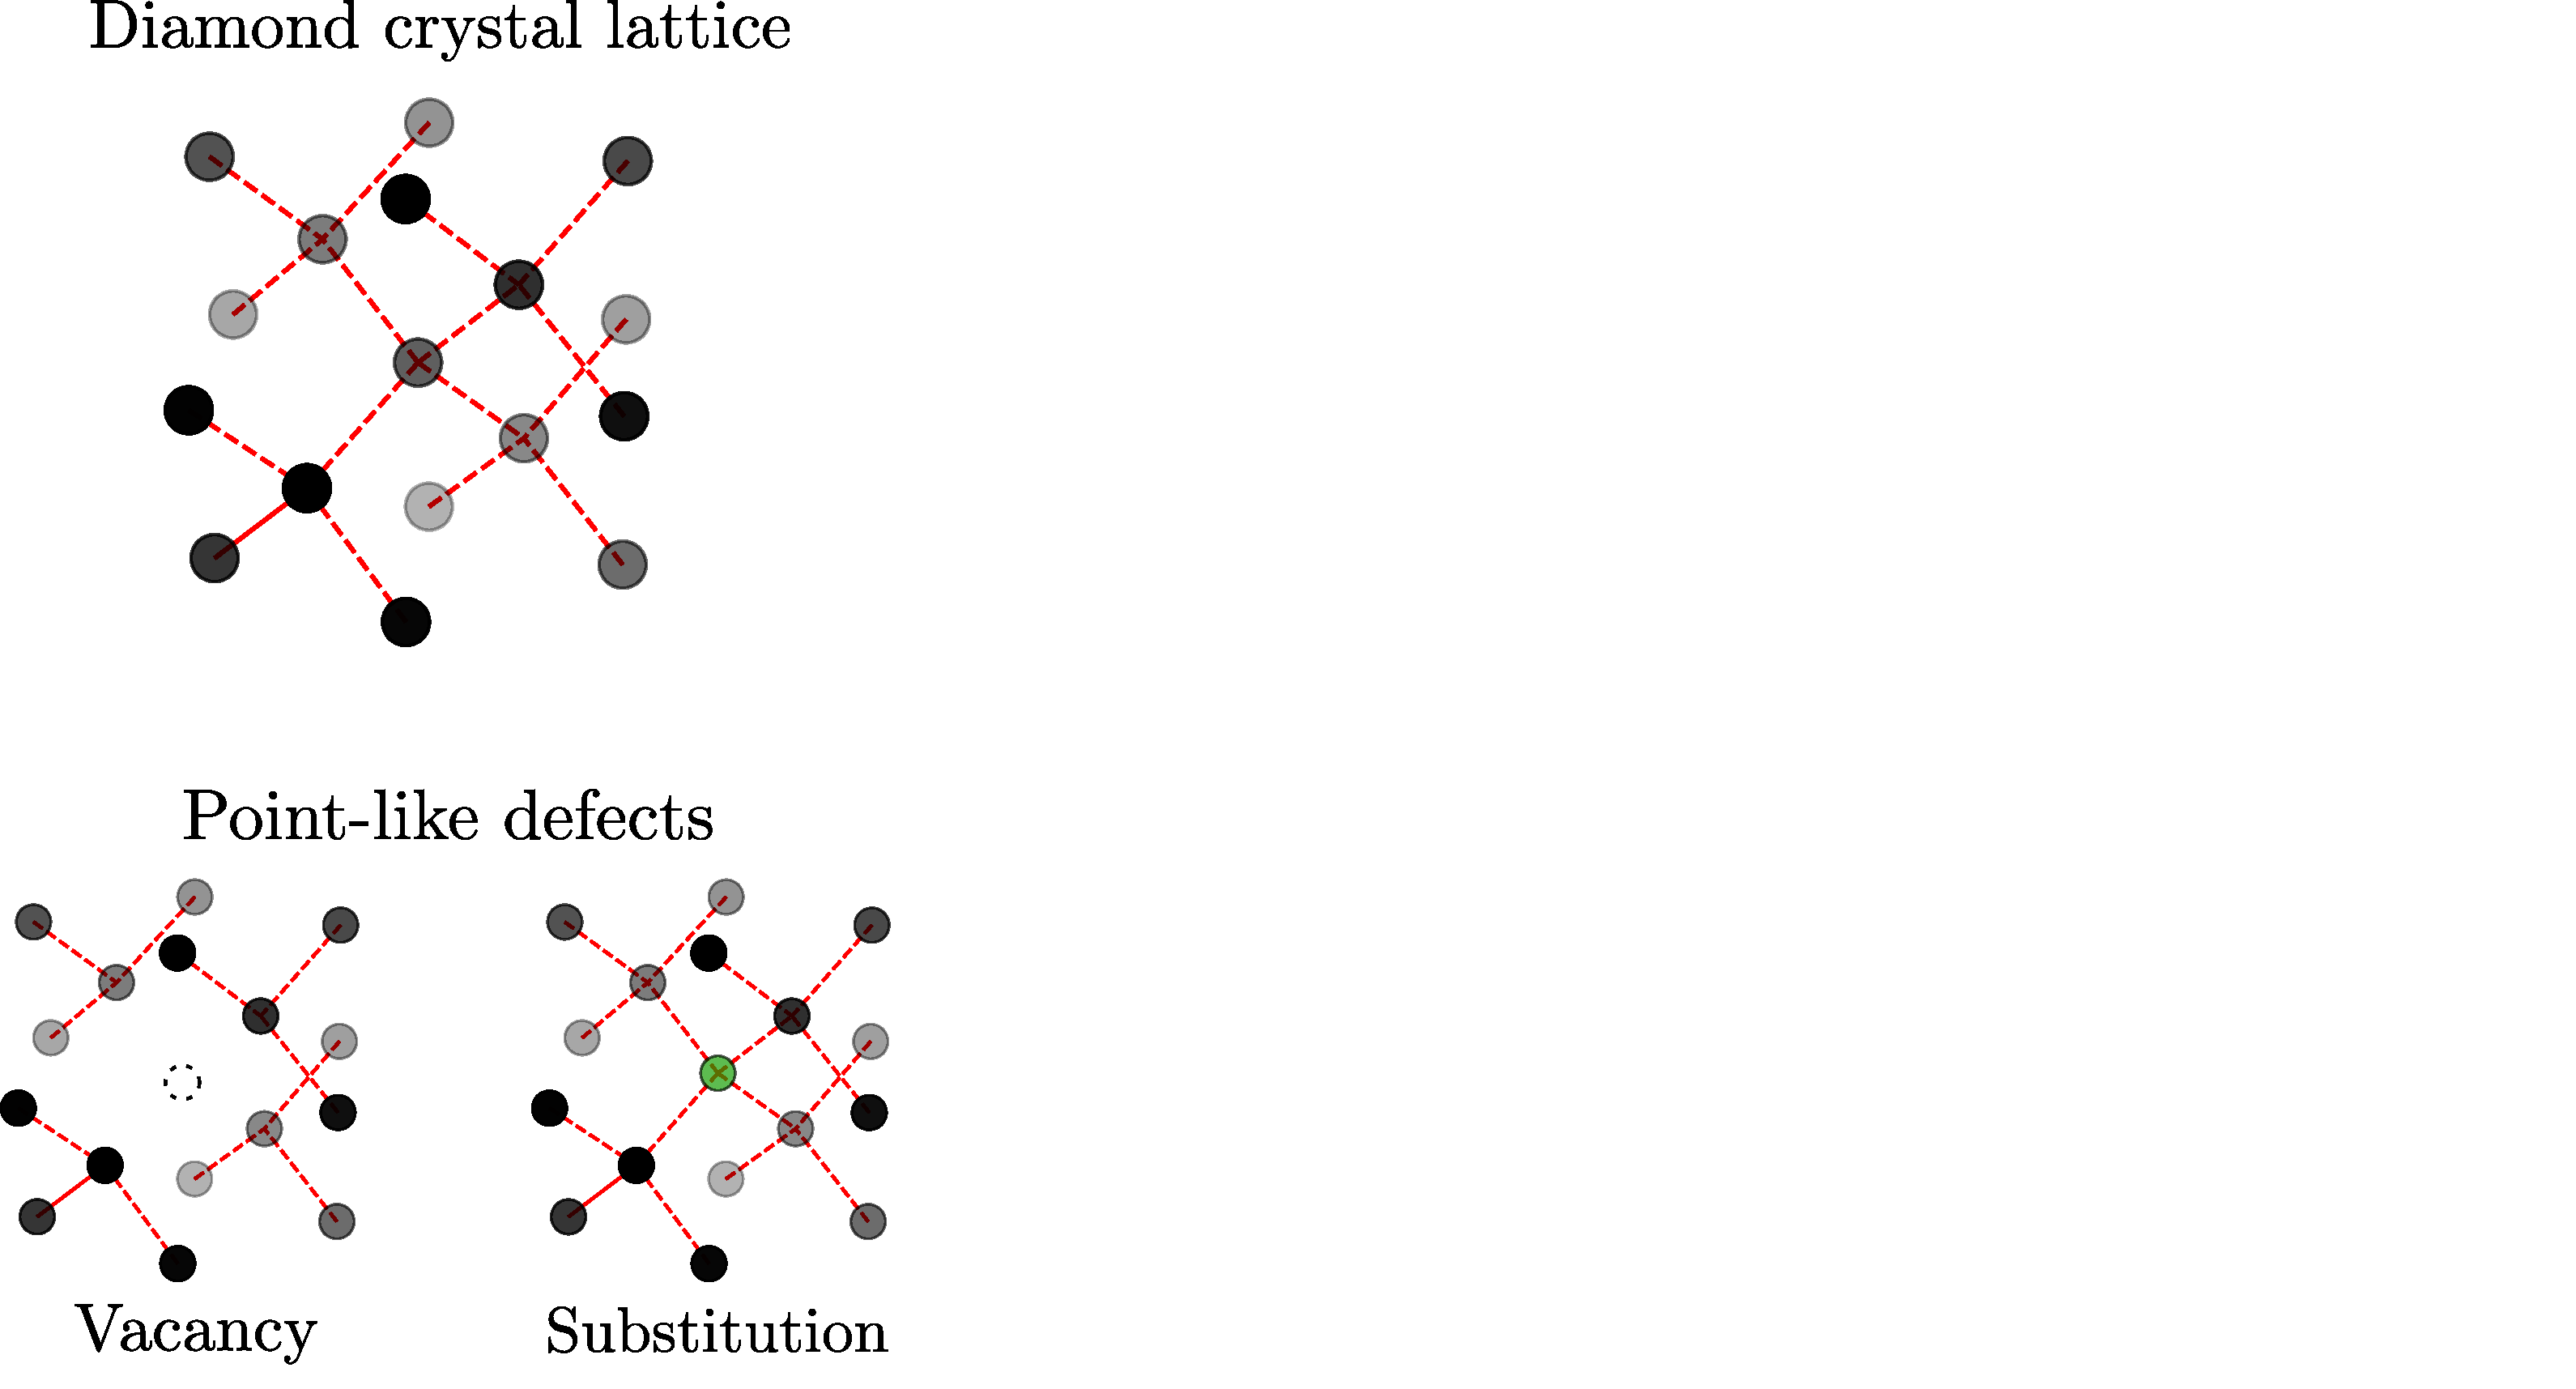
\includegraphics[width=\textwidth,height=0.85\textheight,keepaspectratio]{Slide diamant_0}
\end{frame}

\begin{frame}{Colored centers in diamond}
\centering
\includegraphics[width=\textwidth,height=0.85\textheight,keepaspectratio]{Slide diamant}
\end{frame}

\begin{frame}{Synthetic diamond and NV centers}
\centering
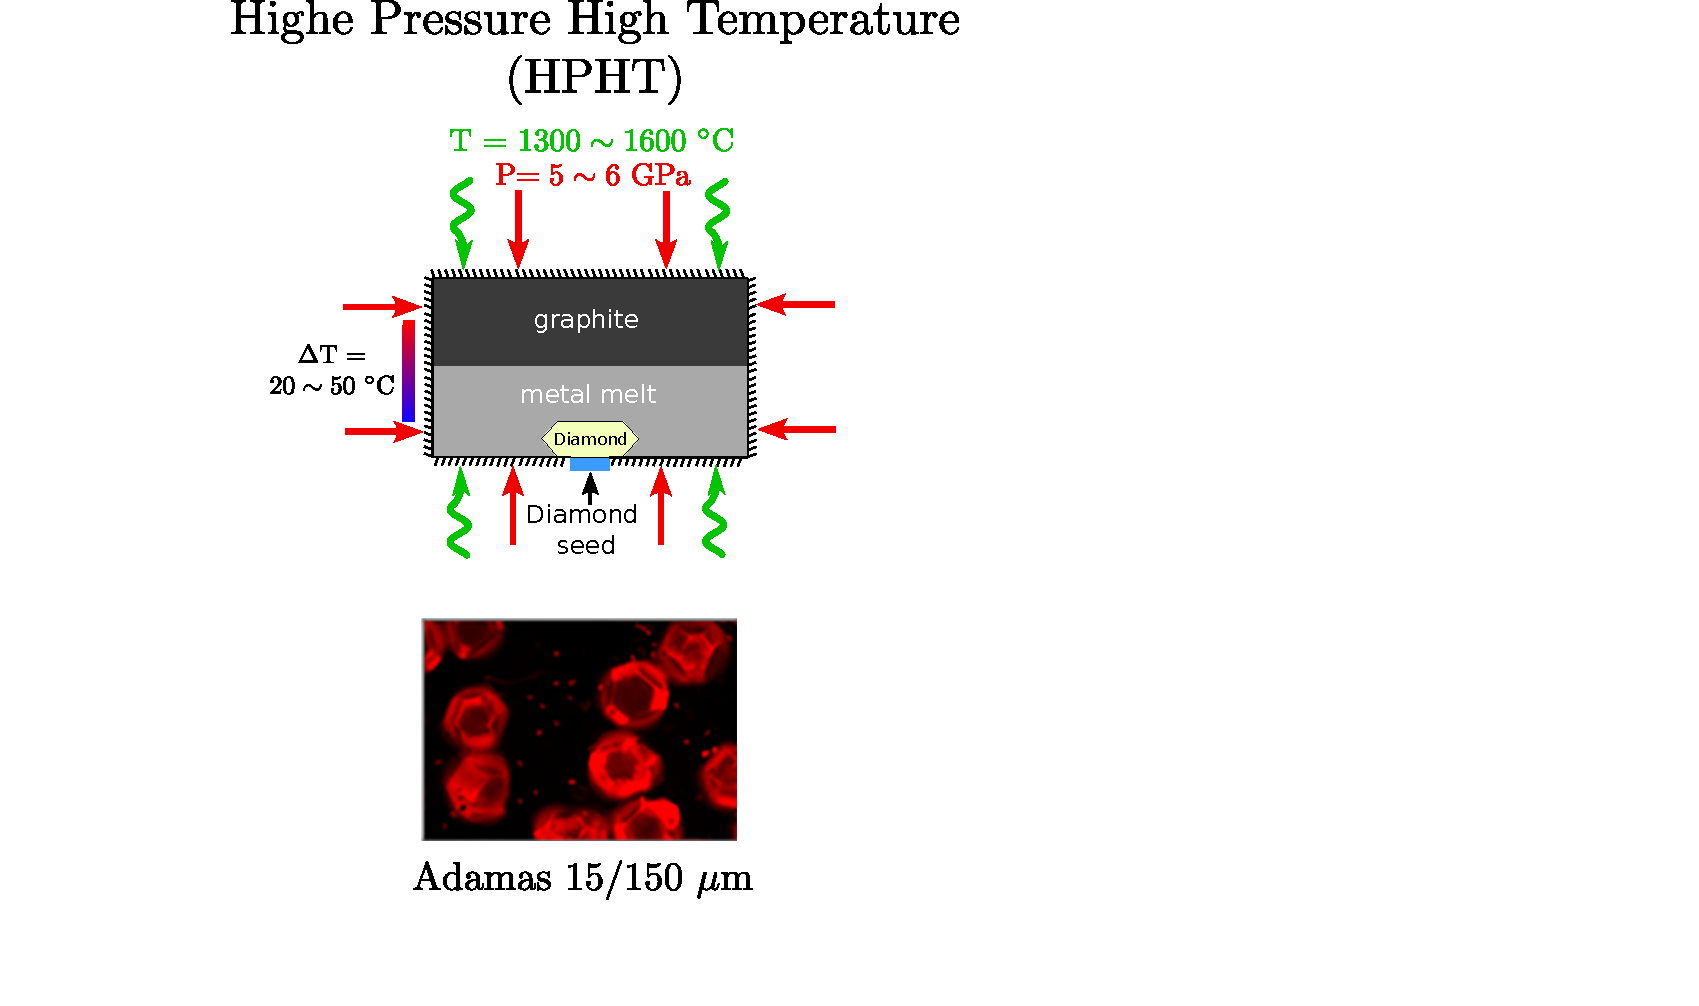
\includegraphics[width=\textwidth,height=0.85\textheight,keepaspectratio]{Slide_fab_sample-3}
\end{frame}

\begin{frame}{Synthetic diamond and NV centers}
\centering
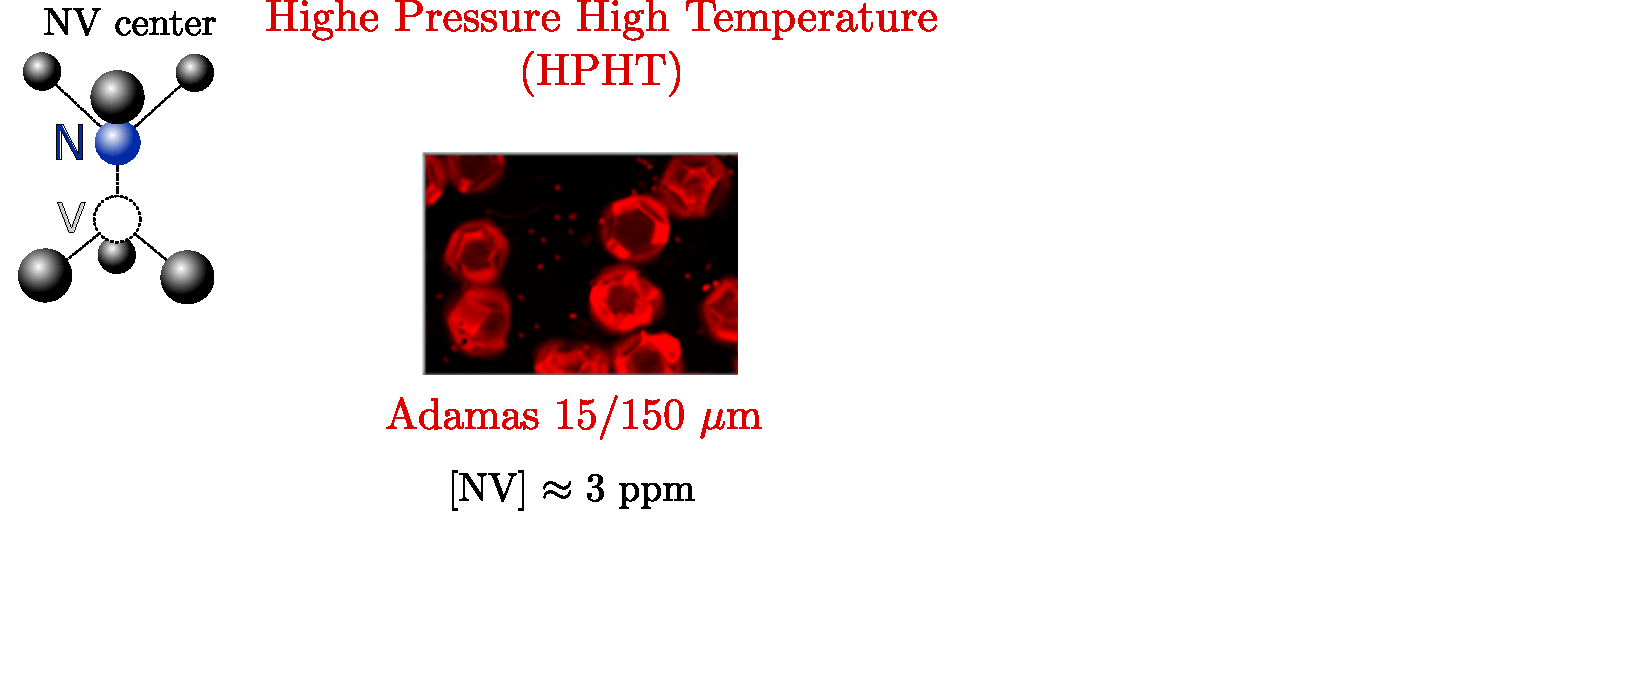
\includegraphics[width=\textwidth,height=0.85\textheight,keepaspectratio]{Slide_fab_sample-2}
\end{frame}

\begin{frame}{Synthetic diamond and NV centers}
\centering
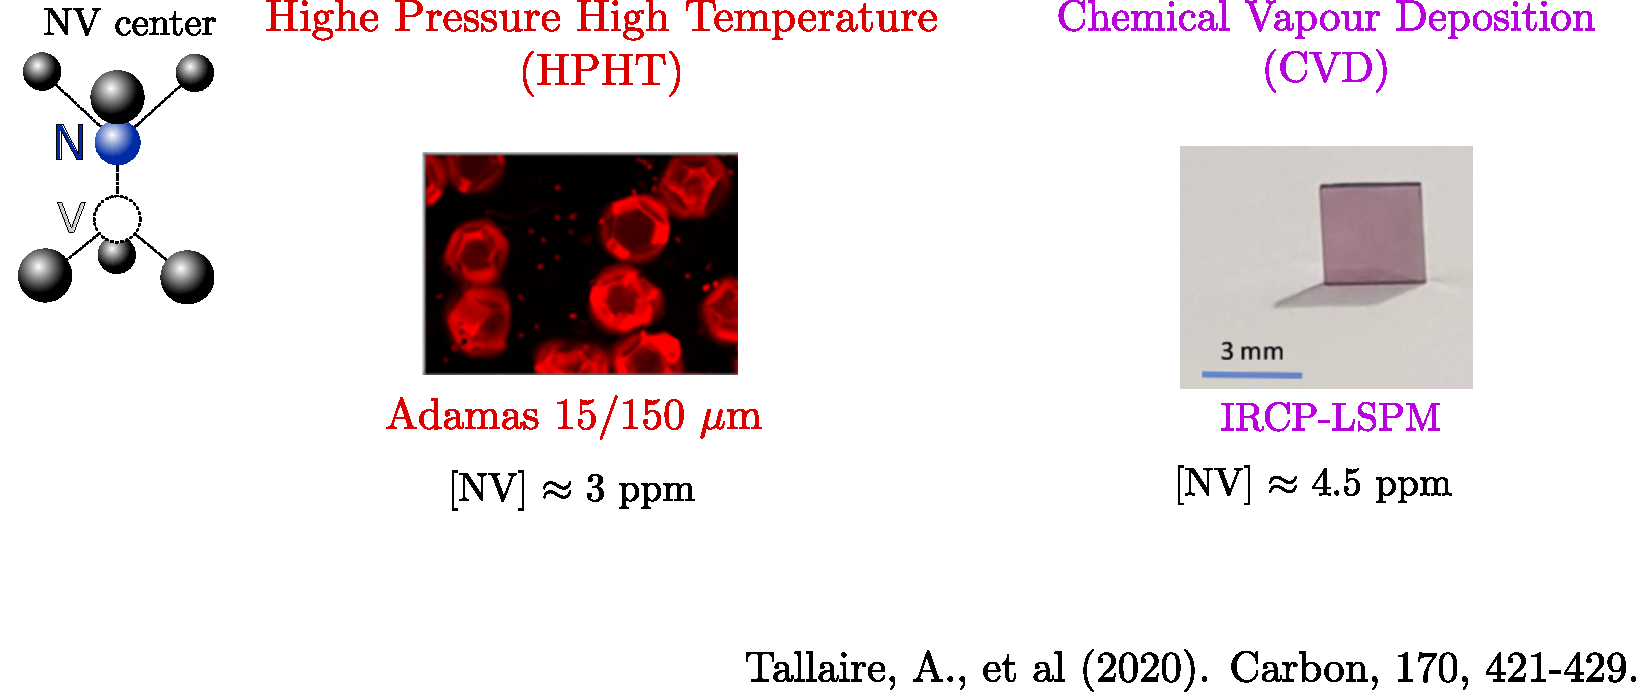
\includegraphics[width=\textwidth,height=0.85\textheight,keepaspectratio]{Slide_fab_sample-1}
\end{frame}

\begin{frame}{Synthetic diamond and NV centers}
\centering
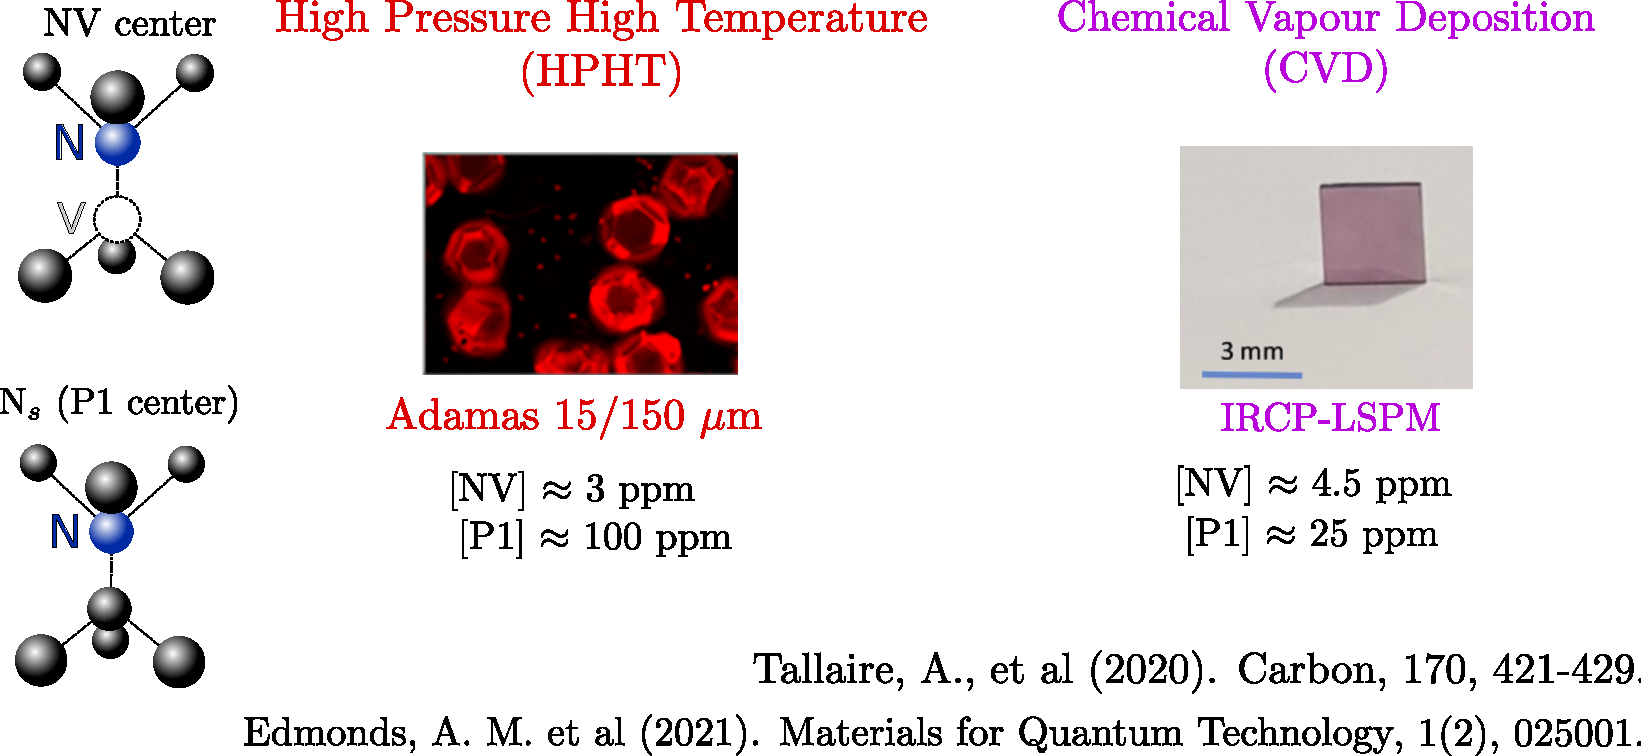
\includegraphics[width=\textwidth,height=0.85\textheight,keepaspectratio]{Slide_fab_sample}
\end{frame}

\subsection{NV center energy levels}
\begin{frame}{The NV center energy levels}
\centering
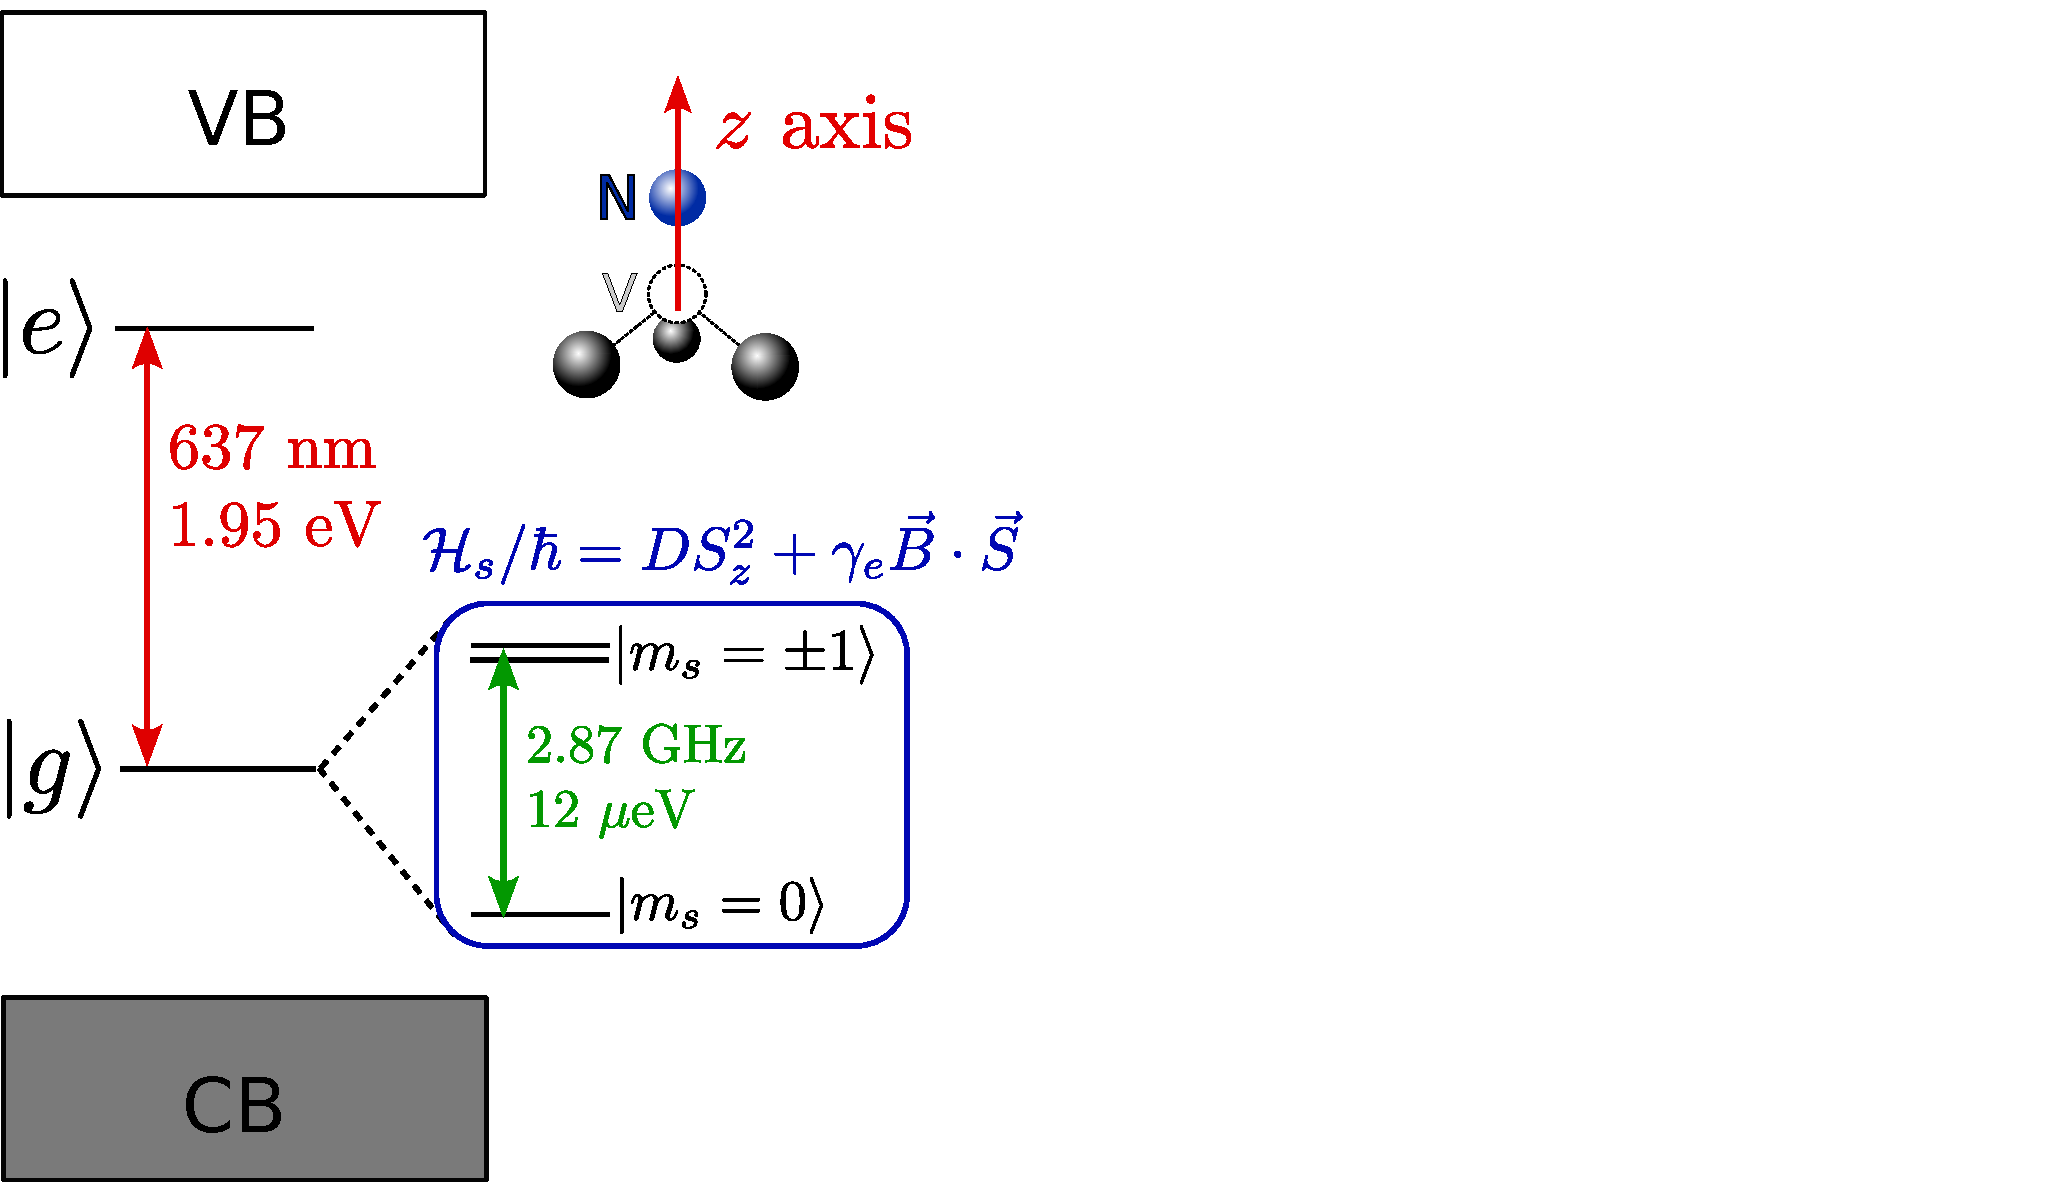
\includegraphics[width=\textwidth,height=0.85\textheight,keepaspectratio]{Slide_NV_levels_3}
\end{frame}

%\begin{frame}{The NV center energy levels}
%\centering
%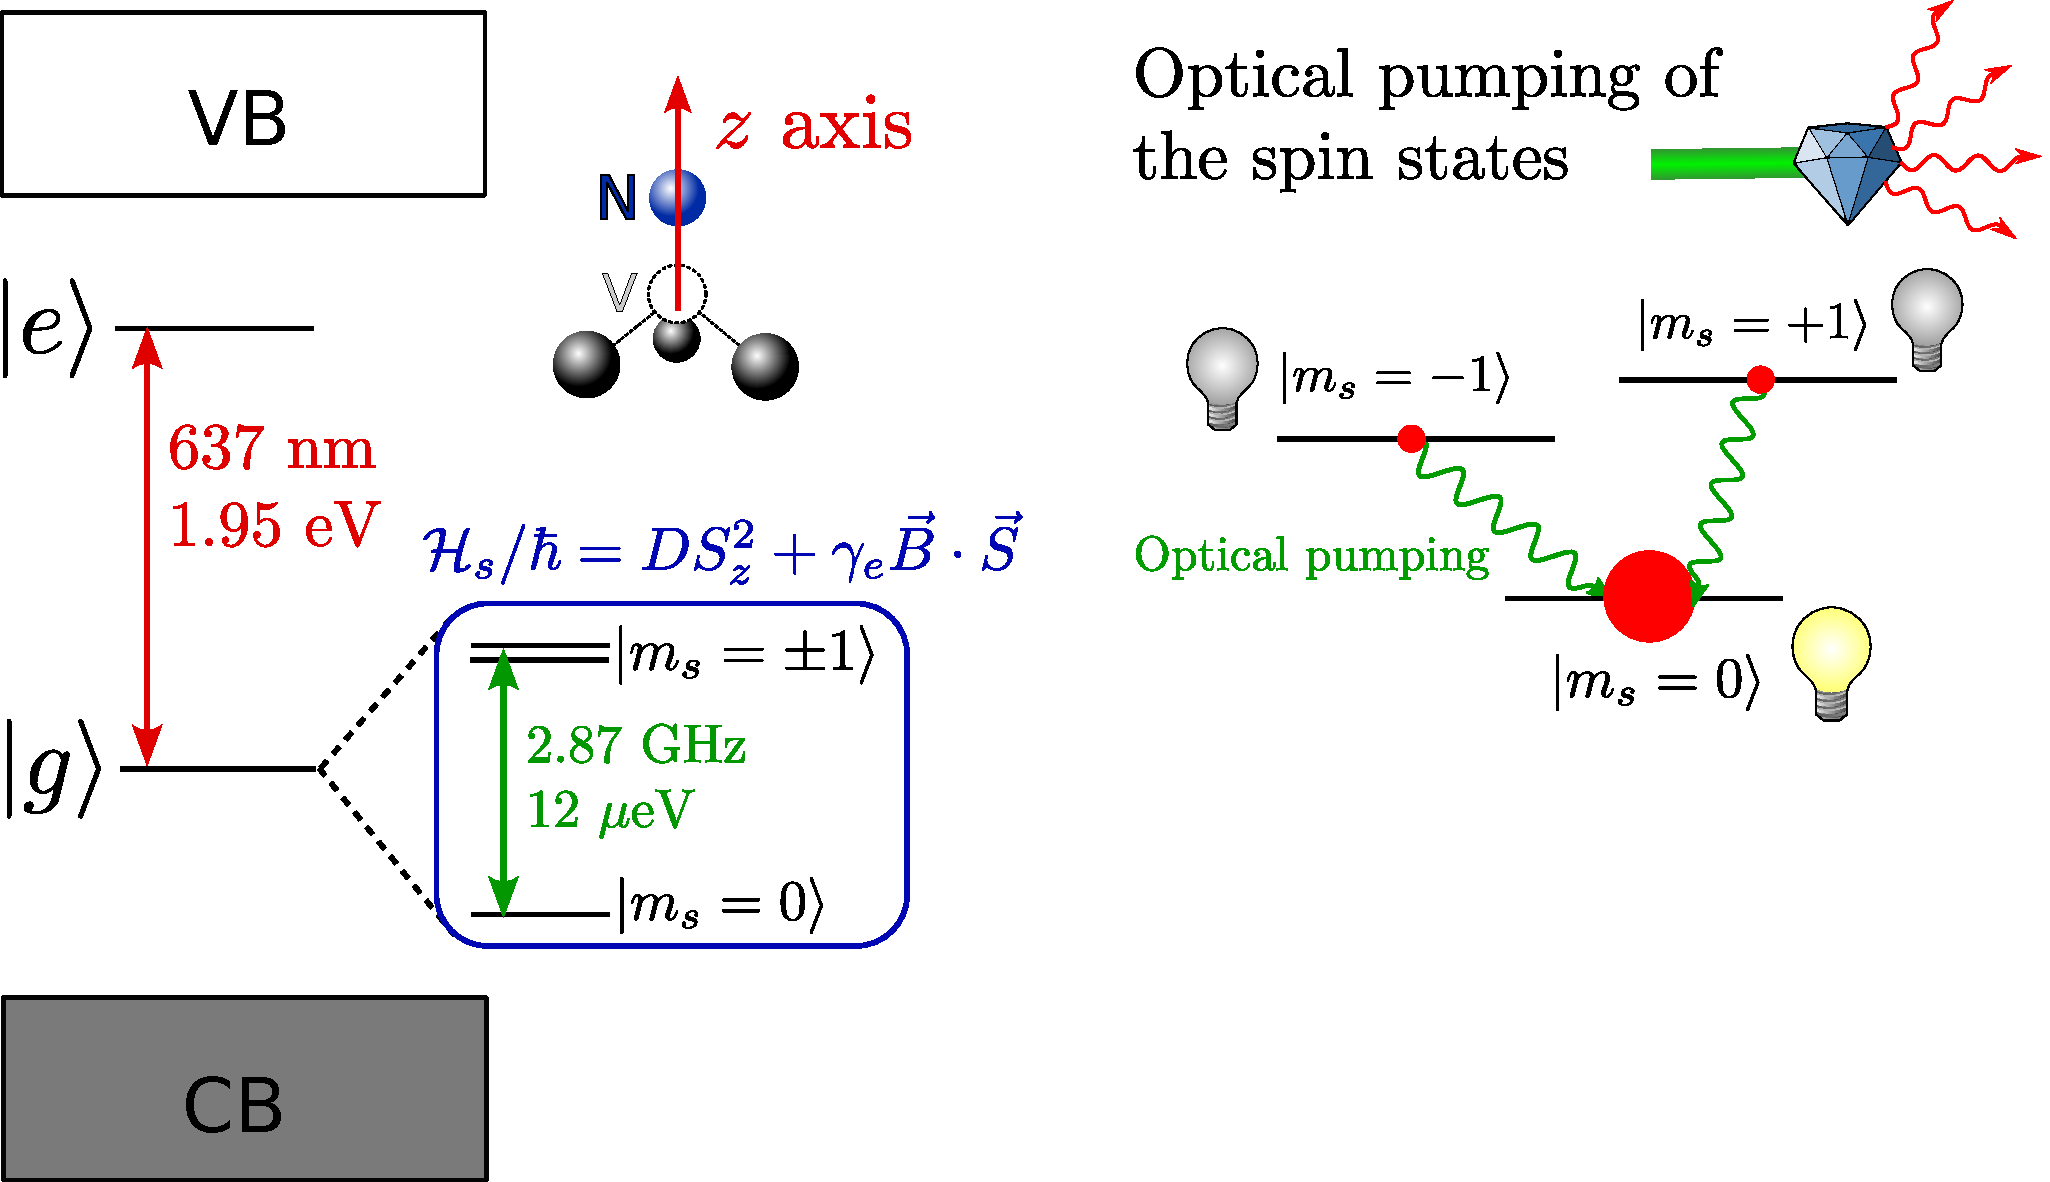
\includegraphics[width=\textwidth,height=0.85\textheight,keepaspectratio]{Slide_NV_levels_2}
%\end{frame}

\begin{frame}{The NV center energy levels}
\centering
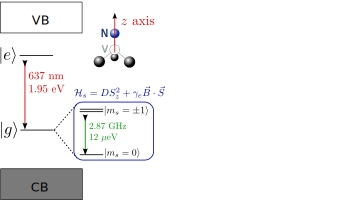
\includegraphics[width=\textwidth,height=0.85\textheight,keepaspectratio]{Slide_NV_levels_1}
\end{frame}

\begin{frame}{The NV center energy levels}
\centering
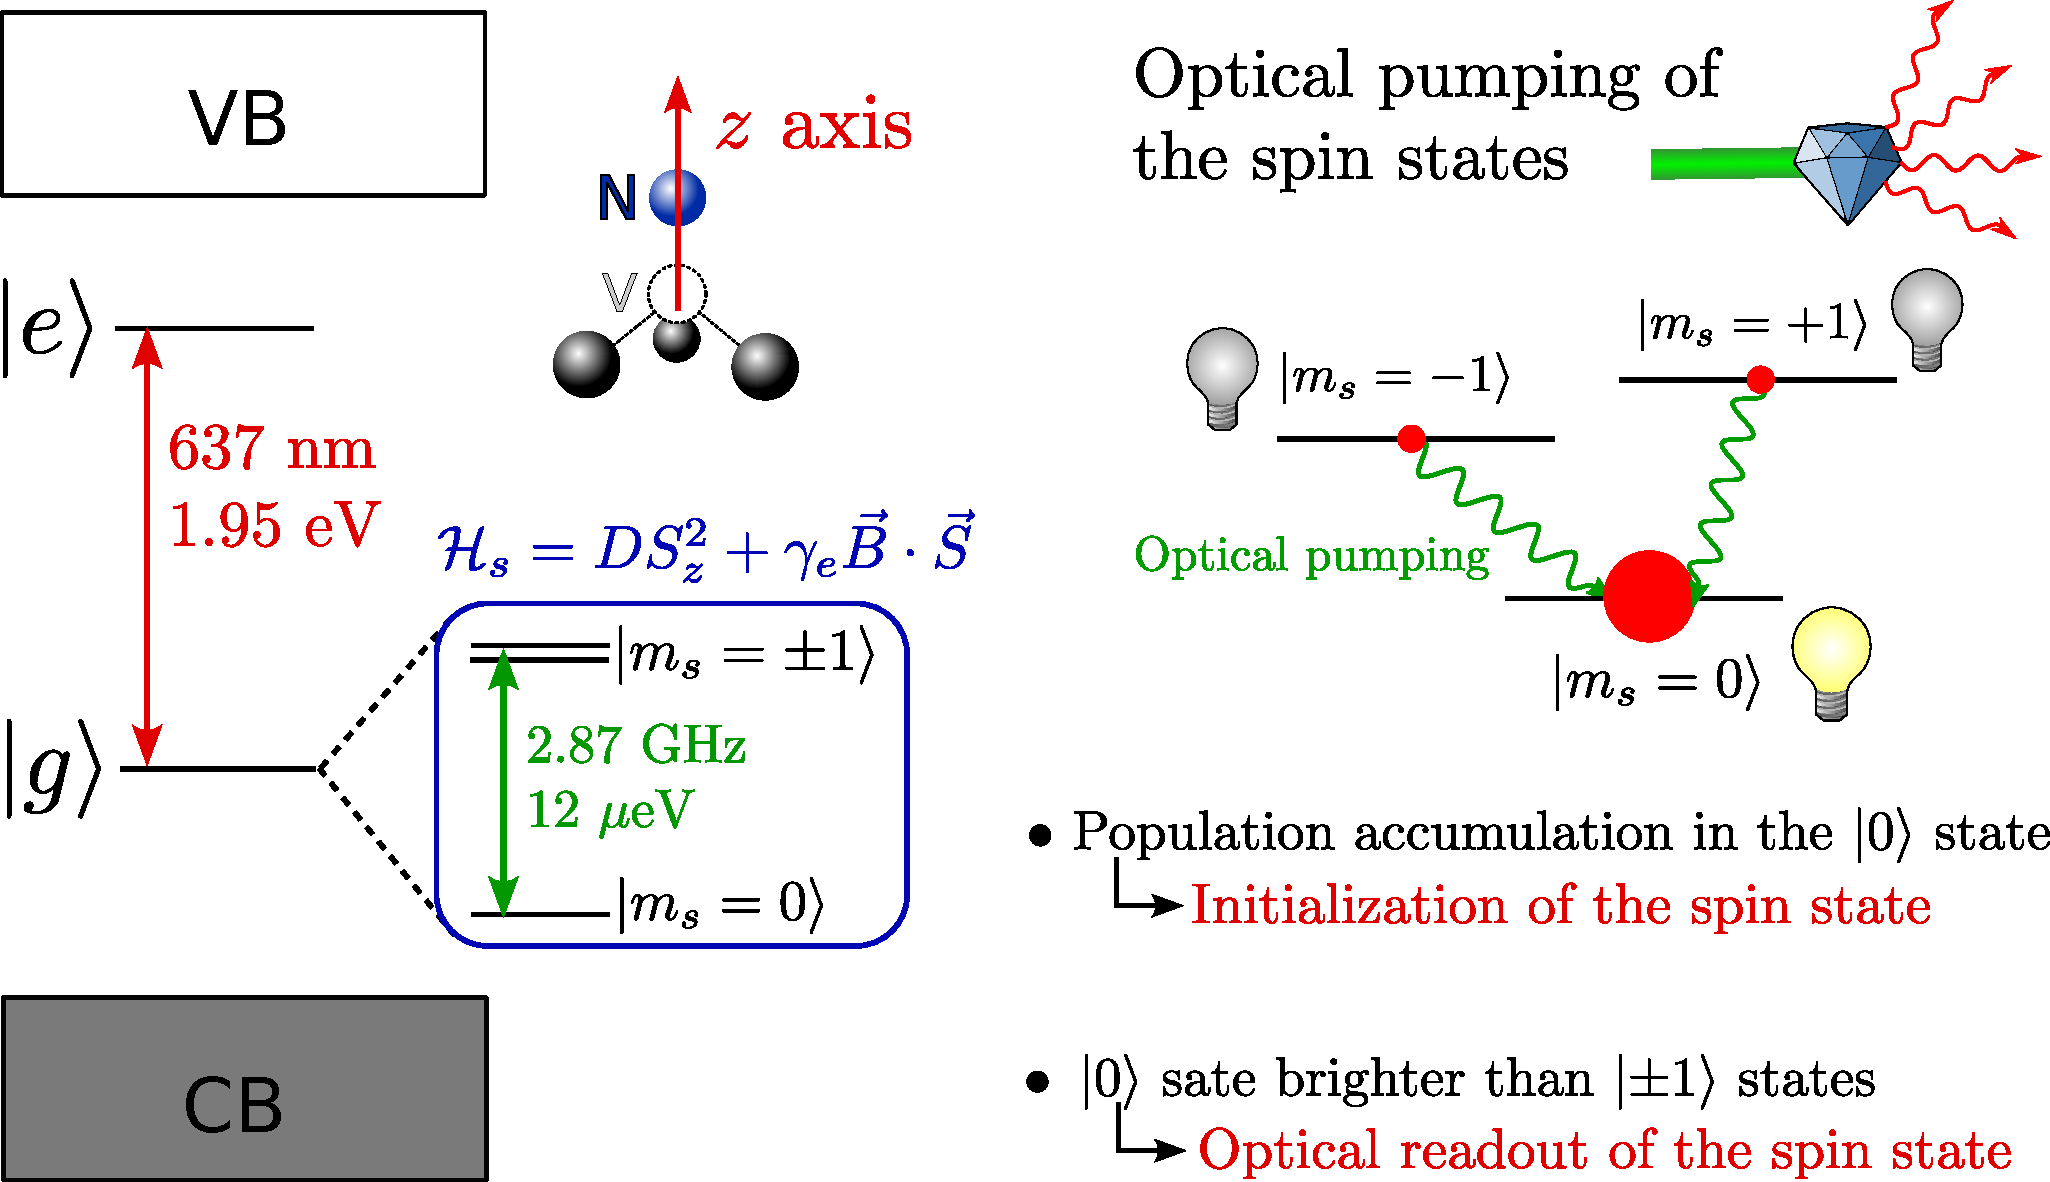
\includegraphics[width=\textwidth,height=0.85\textheight,keepaspectratio]{Slide_NV_levels}
\end{frame}

\subsection{Basic experiment with NV centers}
\begin{frame}{Experimental setup}
\centering
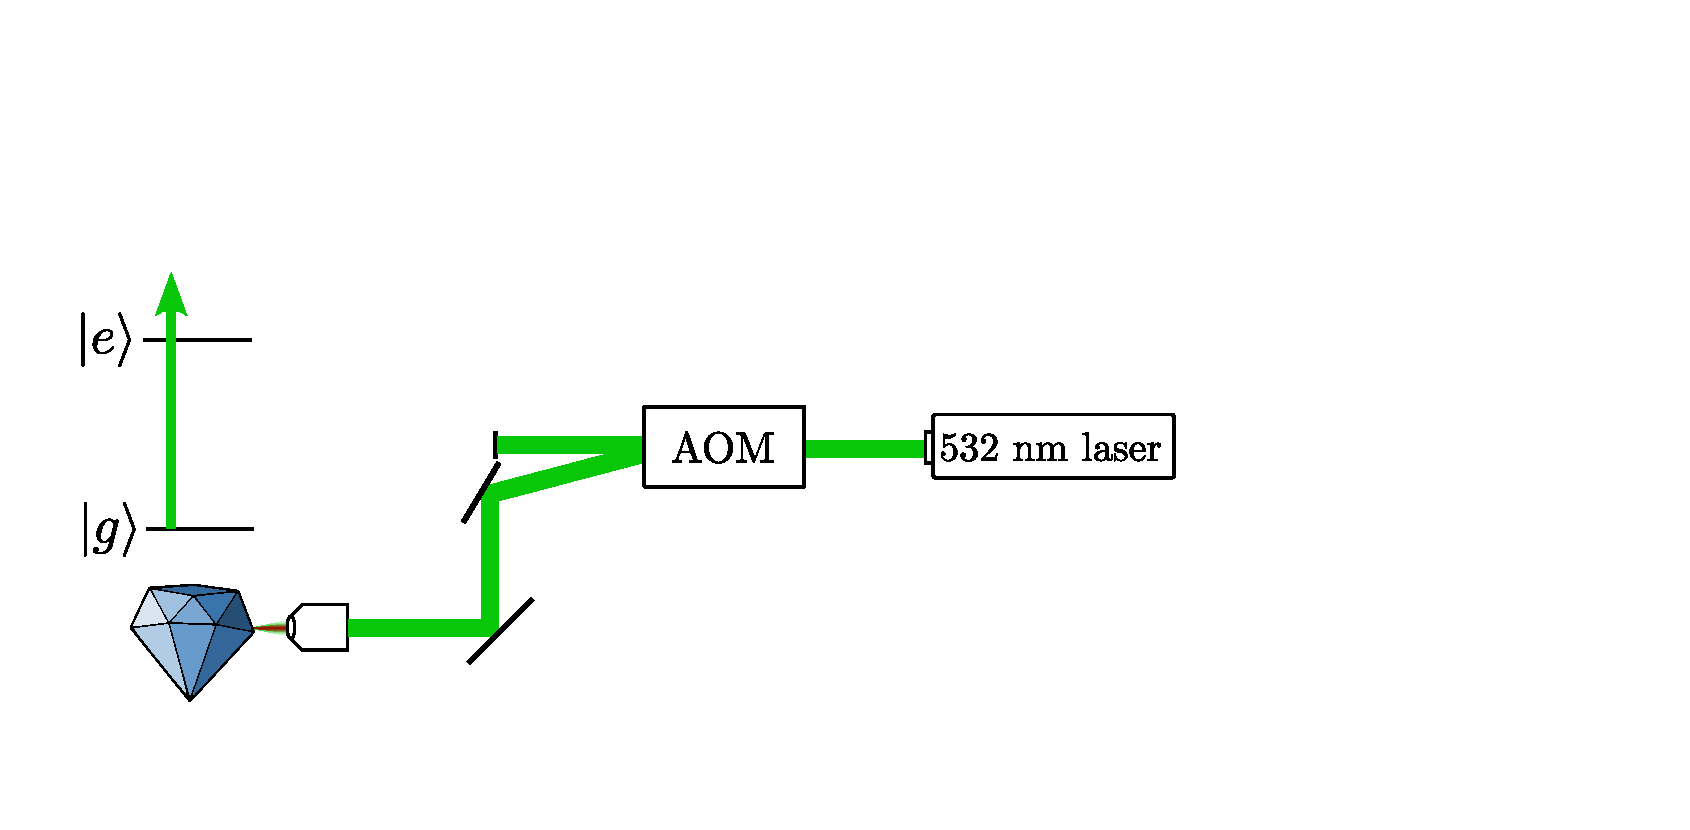
\includegraphics[width=0.9\textwidth,height=0.85\textheight,keepaspectratio]{Slide_setup_-4}
\end{frame}

\begin{frame}{Experimental setup}
\centering
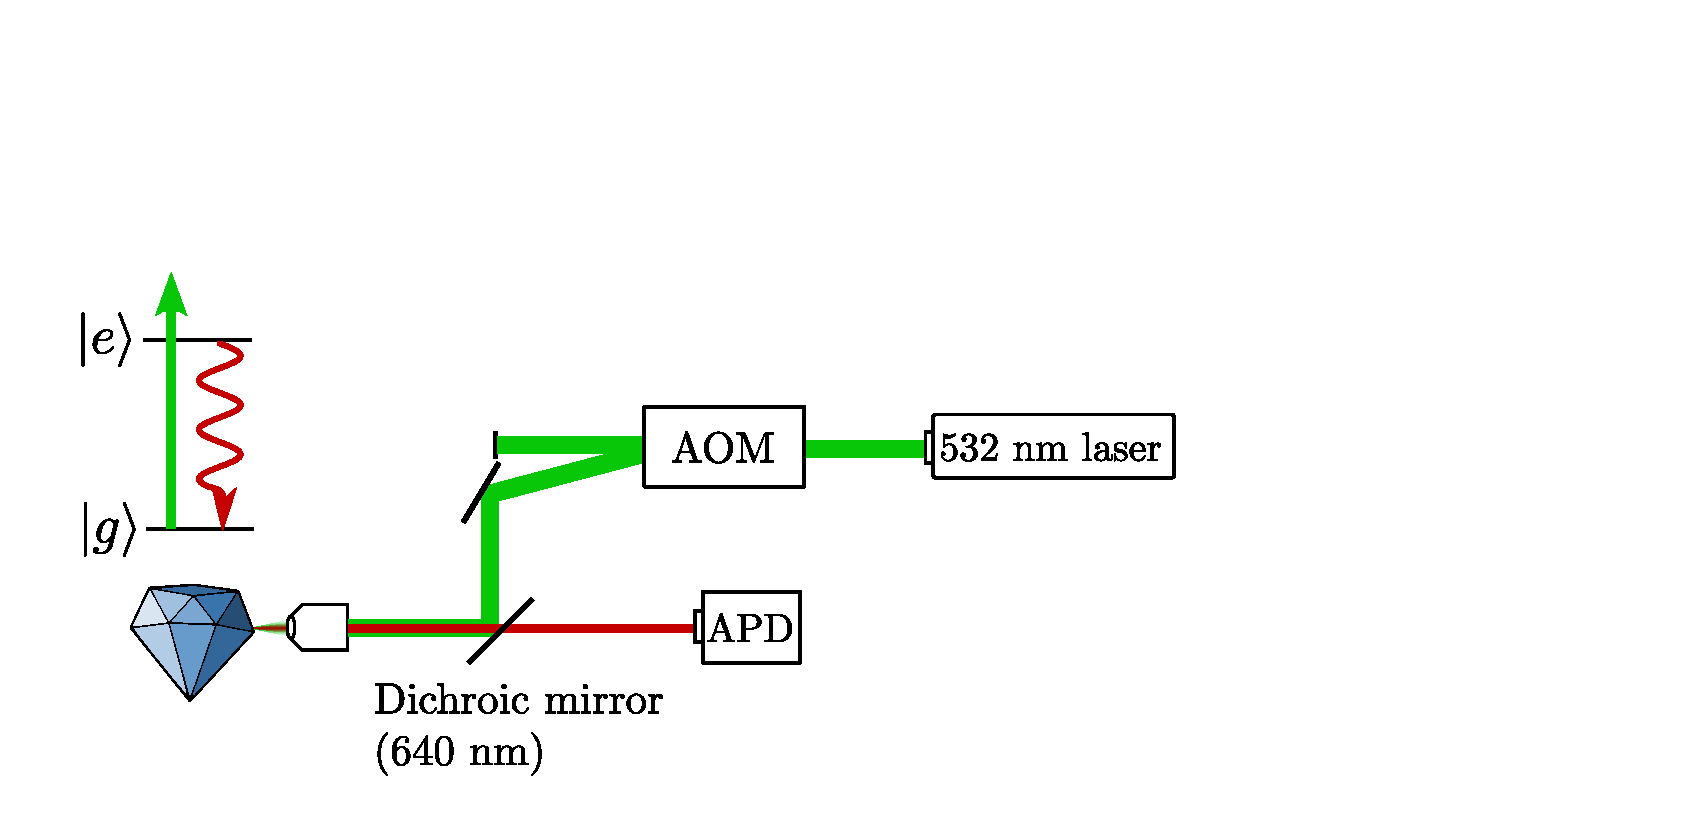
\includegraphics[width=0.9\textwidth,height=0.85\textheight,keepaspectratio]{Slide_setup_-3}
\end{frame}

\begin{frame}{Experimental setup}
\centering
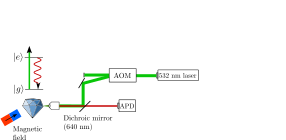
\includegraphics[width=0.9\textwidth,height=0.85\textheight,keepaspectratio]{Slide_setup_-2}
\end{frame}

\begin{frame}{Experimental setup}
\centering
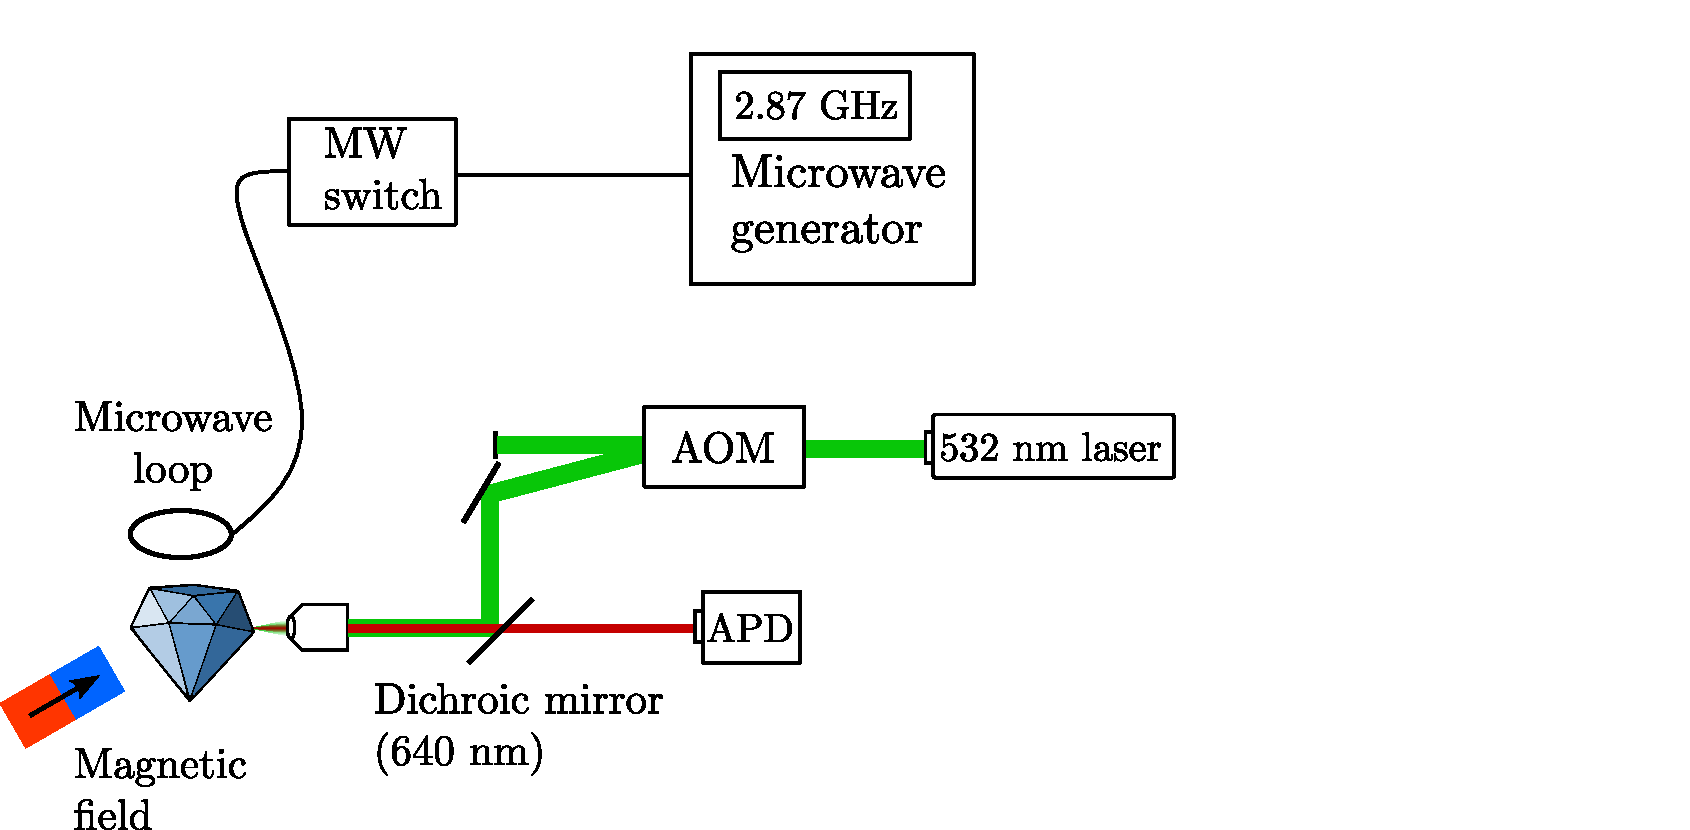
\includegraphics[width=0.9\textwidth,height=0.85\textheight,keepaspectratio]{Slide_setup_-1}
\end{frame}

\begin{frame}{Experimental setup}
\centering
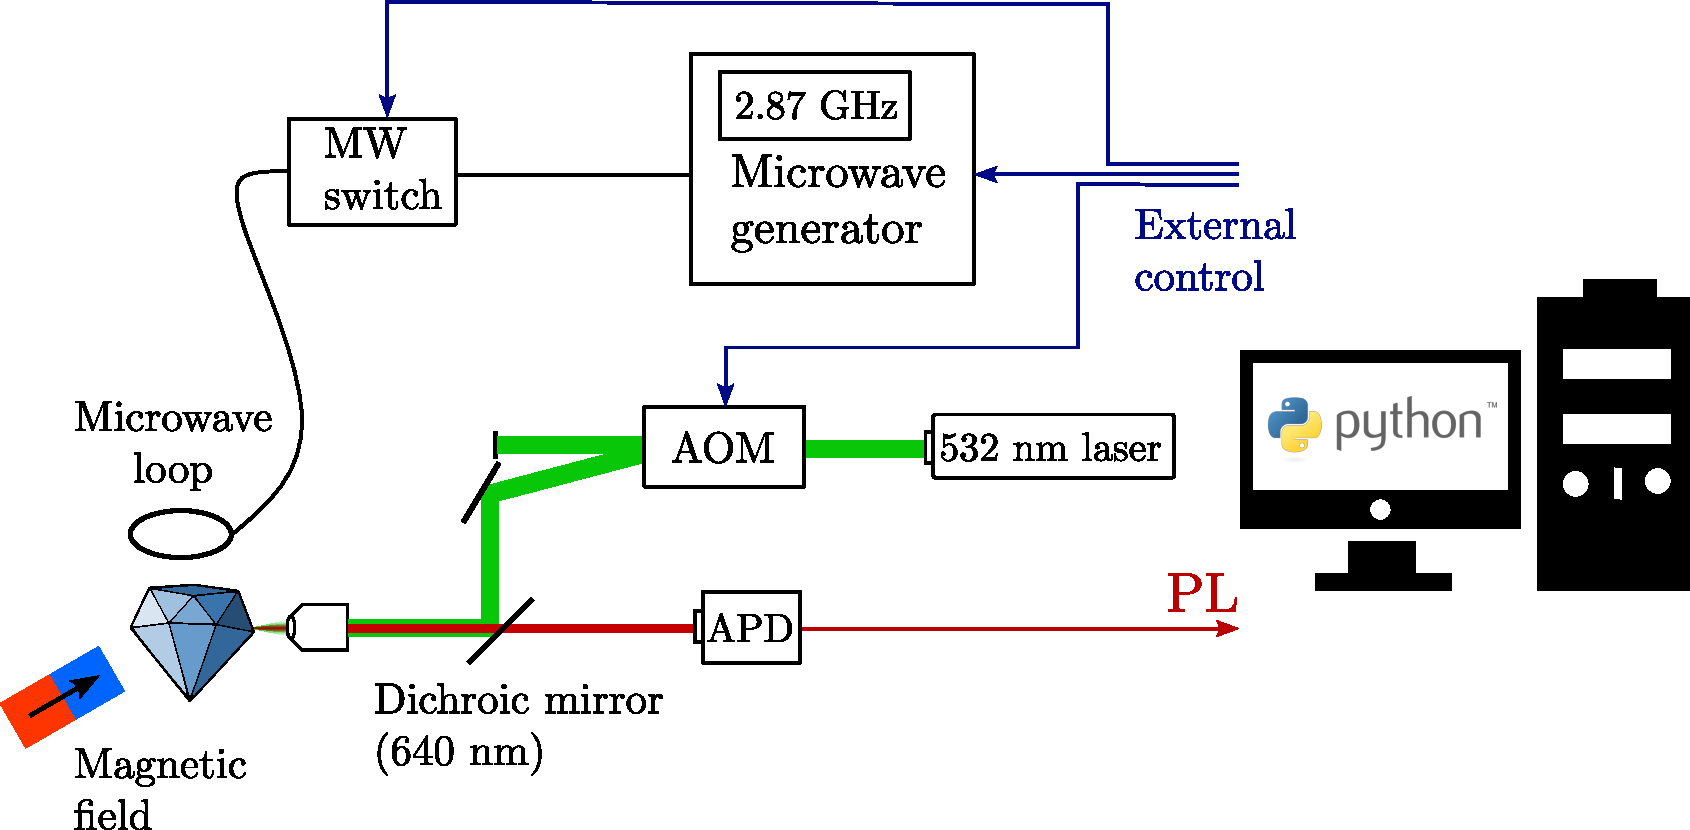
\includegraphics[width=0.9\textwidth,height=0.85\textheight,keepaspectratio]{Slide_setup}
\end{frame}

\begin{frame}{Optically detected magnetic resonance (ODMR)}
\centering
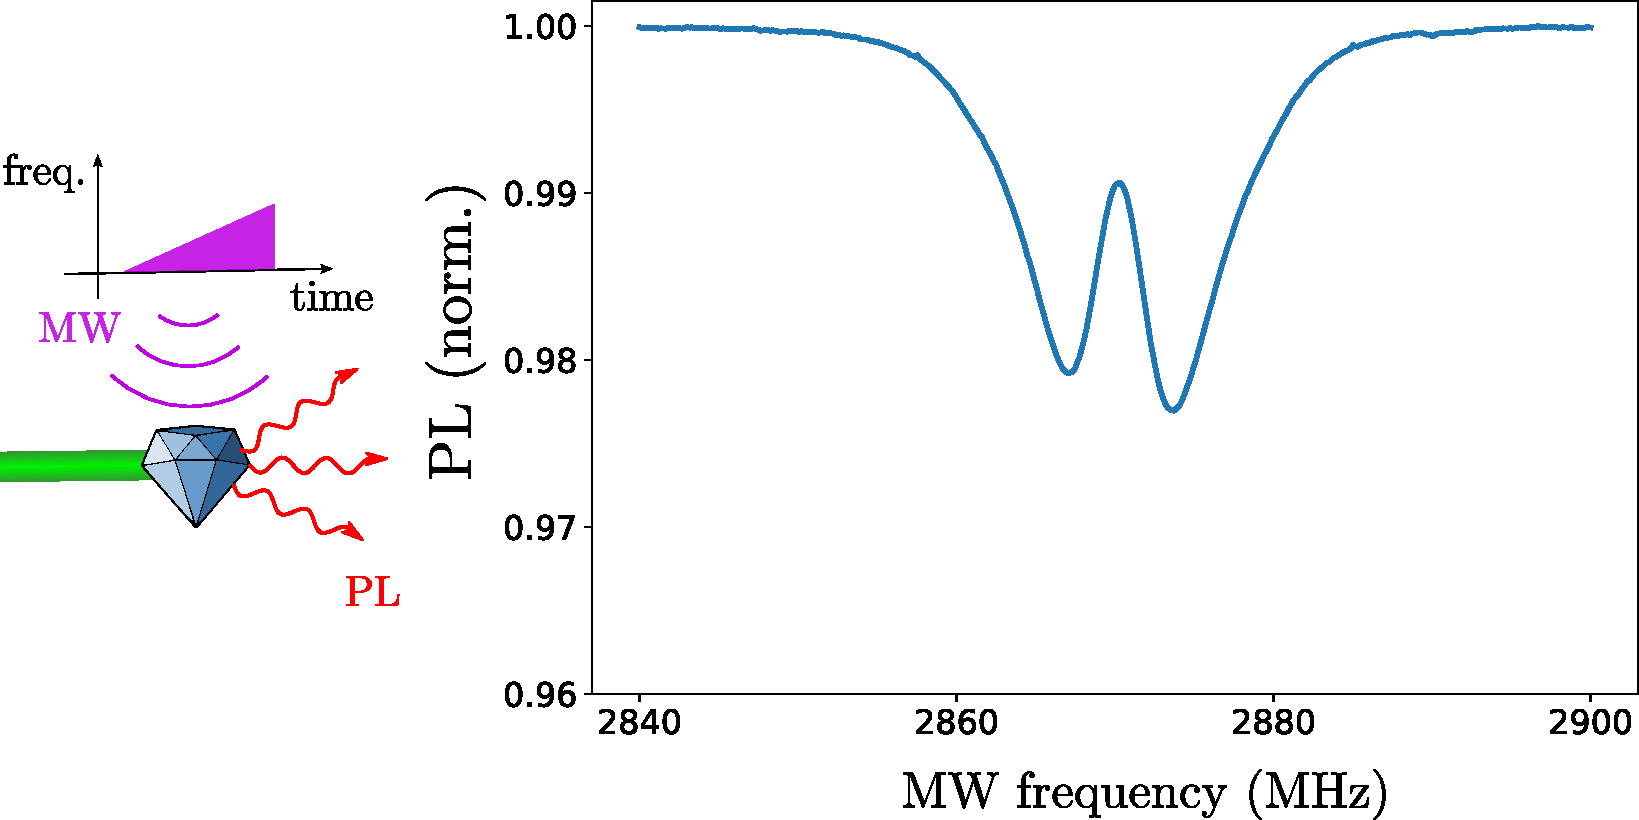
\includegraphics[width=\textwidth,height=0.80\textheight,keepaspectratio]{Slide_ODMR_0_-3}
\end{frame}

\begin{frame}{Optically detected magnetic resonance (ODMR)}
\centering
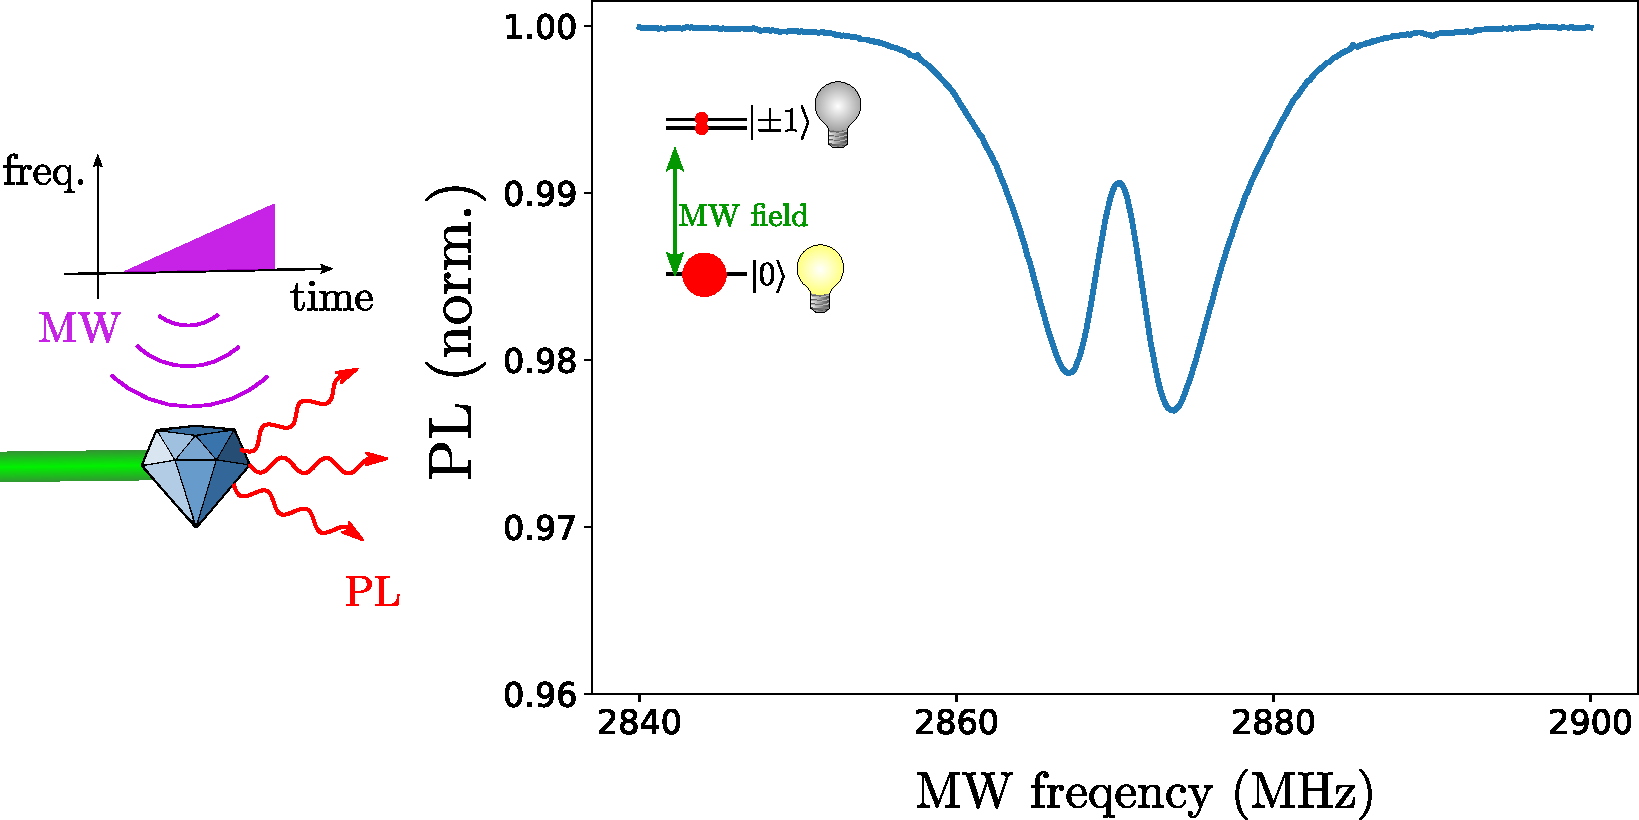
\includegraphics[width=\textwidth,height=0.80\textheight,keepaspectratio]{Slide_ODMR_0_-2}
\end{frame}

\begin{frame}{Optically detected magnetic resonance (ODMR)}
\centering
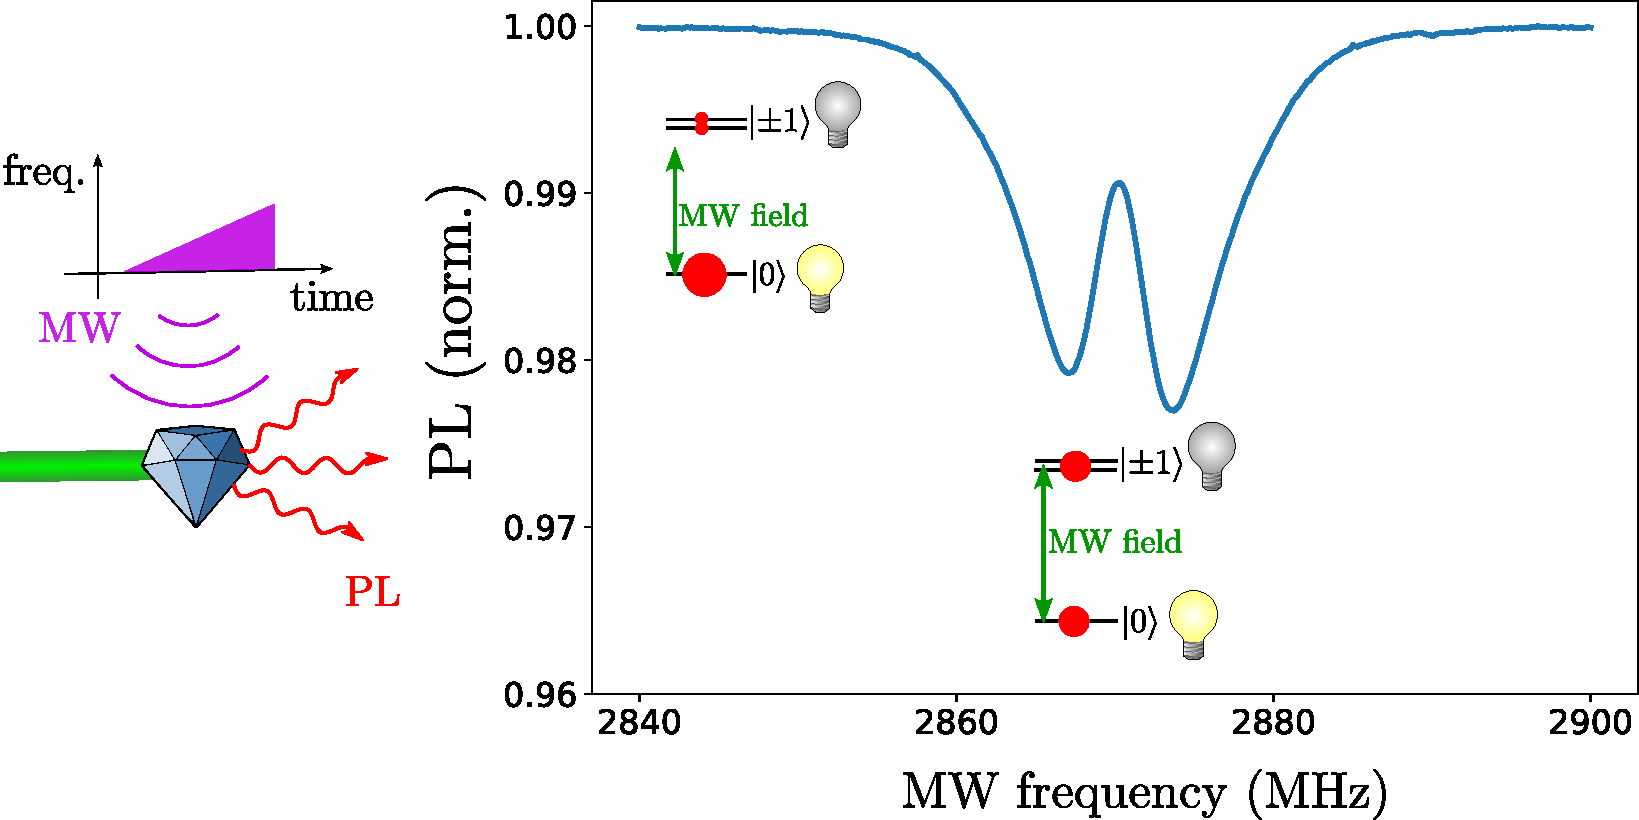
\includegraphics[width=\textwidth,height=0.80\textheight,keepaspectratio]{Slide_ODMR_0_-1}
\end{frame}

\begin{frame}{Optically detected magnetic resonance (ODMR)}
\centering
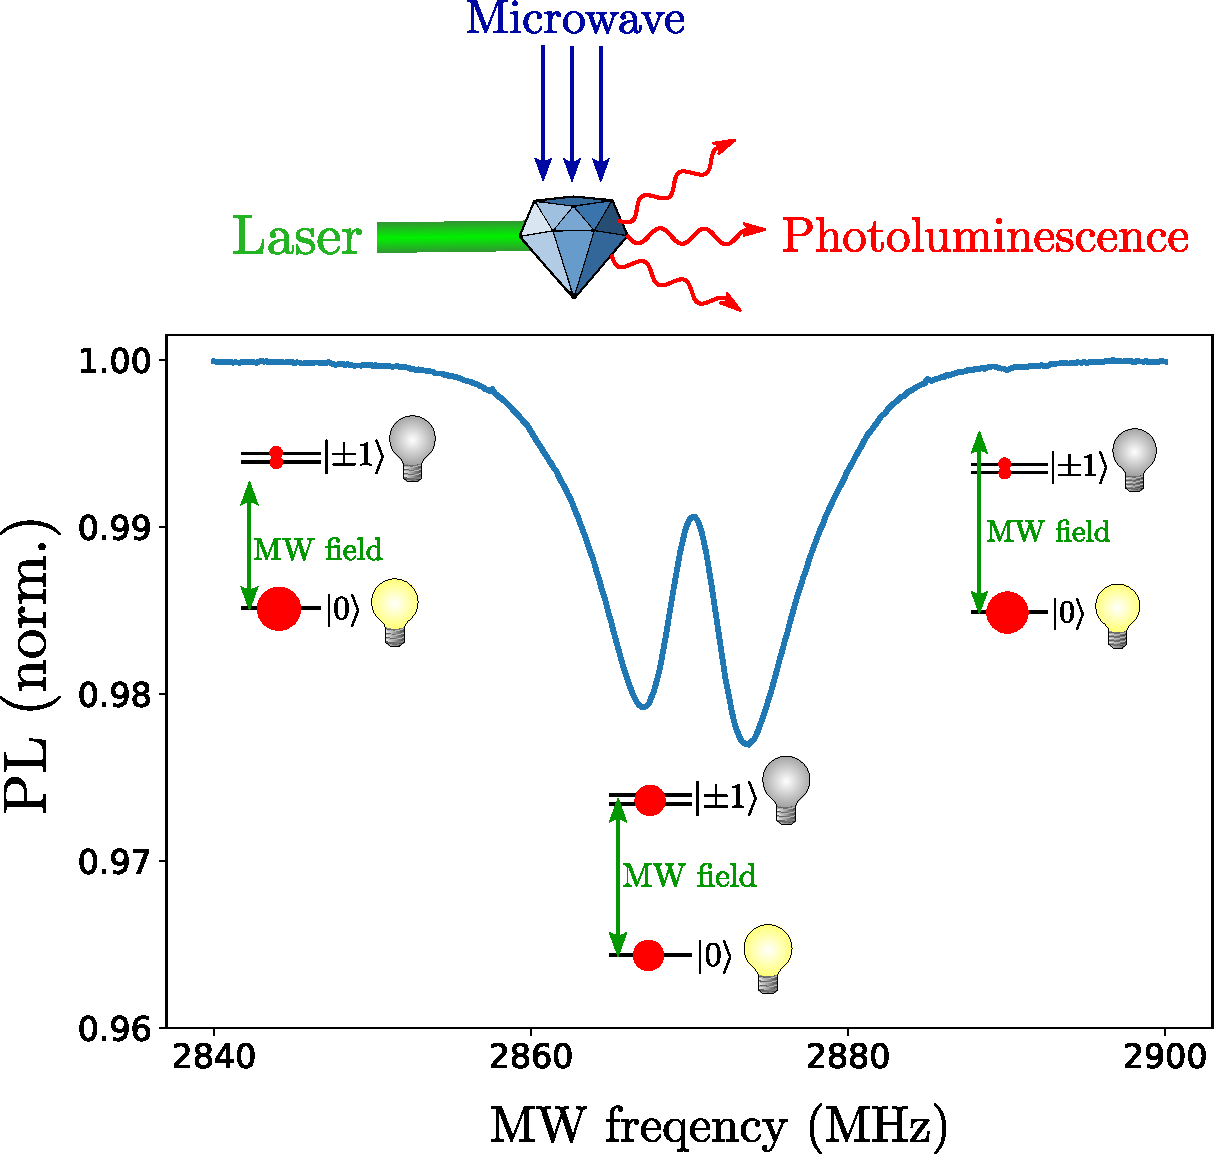
\includegraphics[width=\textwidth,height=0.80\textheight,keepaspectratio]{Slide_ODMR_0}
\end{frame}

\begin{frame}{ODMR with NV ensemble: the 4 classes}
\centering
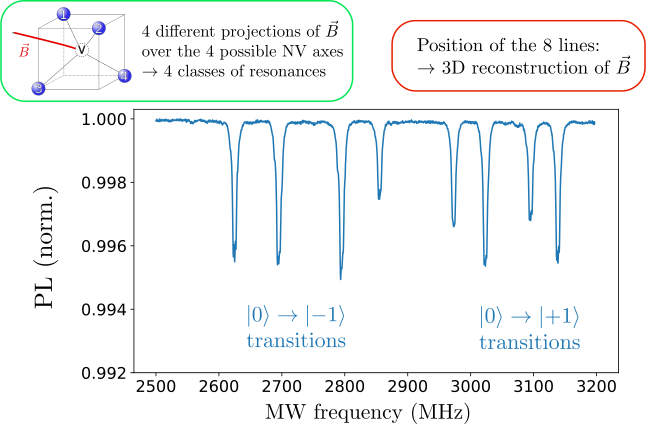
\includegraphics[width=\textwidth,height=0.85\textheight,keepaspectratio]{Slide_ODMR_8_classes}
\end{frame}

\begin{frame}{Transverse magnetic field effect}
\centering
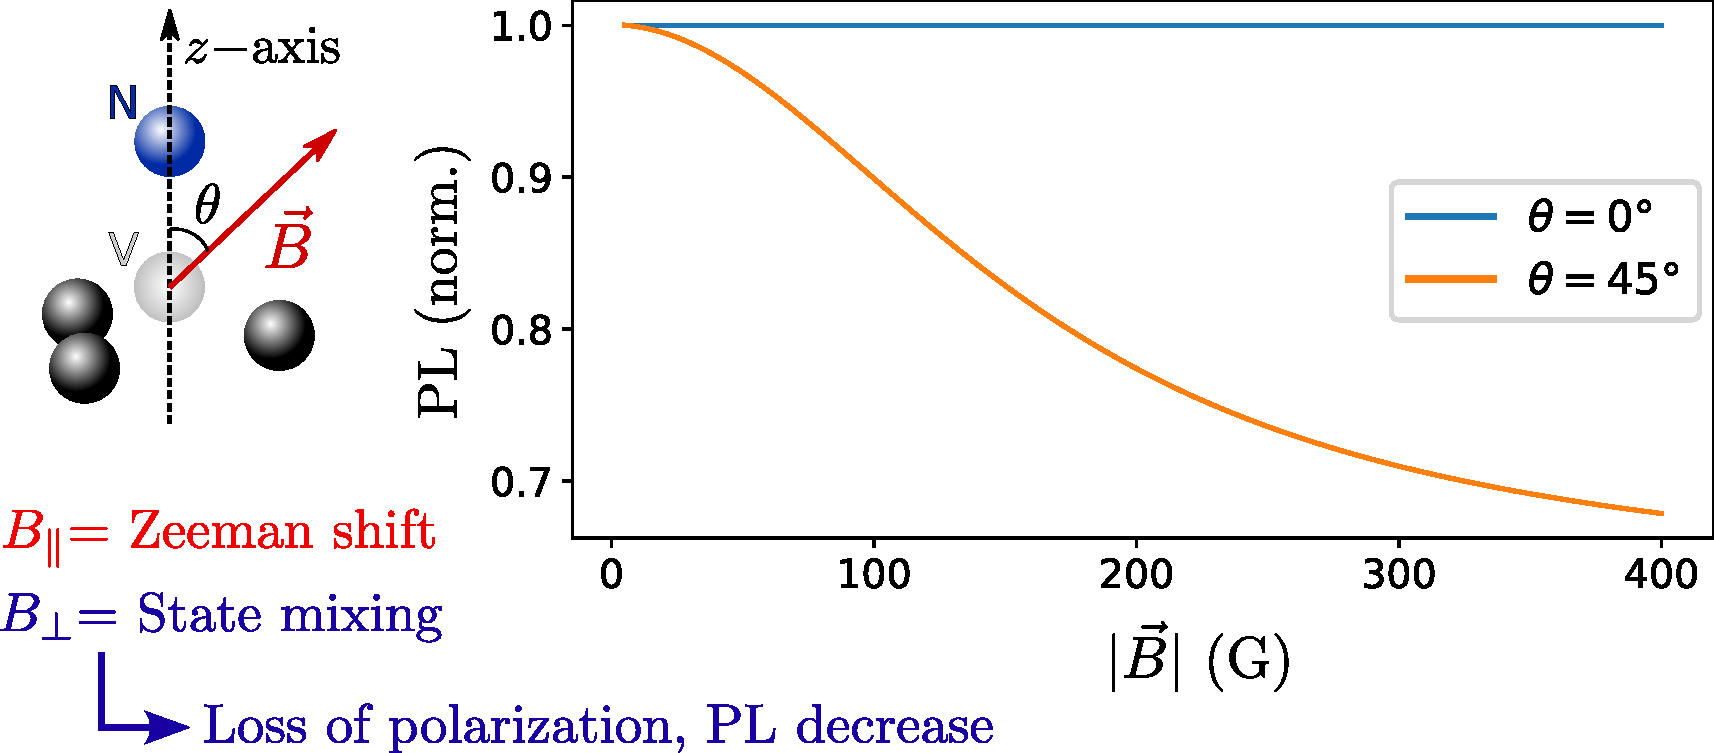
\includegraphics[width=\textwidth,height=0.85\textheight,keepaspectratio]{Slide_champs_transverse_allege}
\end{frame}



\section{Low field depolarization magnetometry (LFDM)}
\subsection{Principle}
\begin{frame}{Outline}
\tableofcontents[currentsection]
\end{frame}

\begin{frame}{Depolarization of dense NV ensemble at low magnetic field}
\centering
\includegraphics[width=\textwidth,height=0.85\textheight,keepaspectratio]{slide_low_field_depolarization_f_-3}
\end{frame}

\begin{frame}{Depolarization of dense NV ensemble at low magnetic field}
\centering
\includegraphics[width=\textwidth,height=0.85\textheight,keepaspectratio]{slide_low_field_depolarization_f_-2}
\end{frame}

\begin{frame}{Depolarization of dense NV ensemble at low magnetic field}
\centering
\includegraphics[width=\textwidth,height=0.85\textheight,keepaspectratio]{slide_low_field_depolarization_f_-1}
\end{frame}

\begin{frame}{Depolarization of dense NV ensemble at low magnetic field}
\centering
\includegraphics[width=\textwidth,height=0.85\textheight,keepaspectratio]{slide_low_field_depolarization_f}
\end{frame}

\begin{frame}{LFDM experimental setup}
\centering
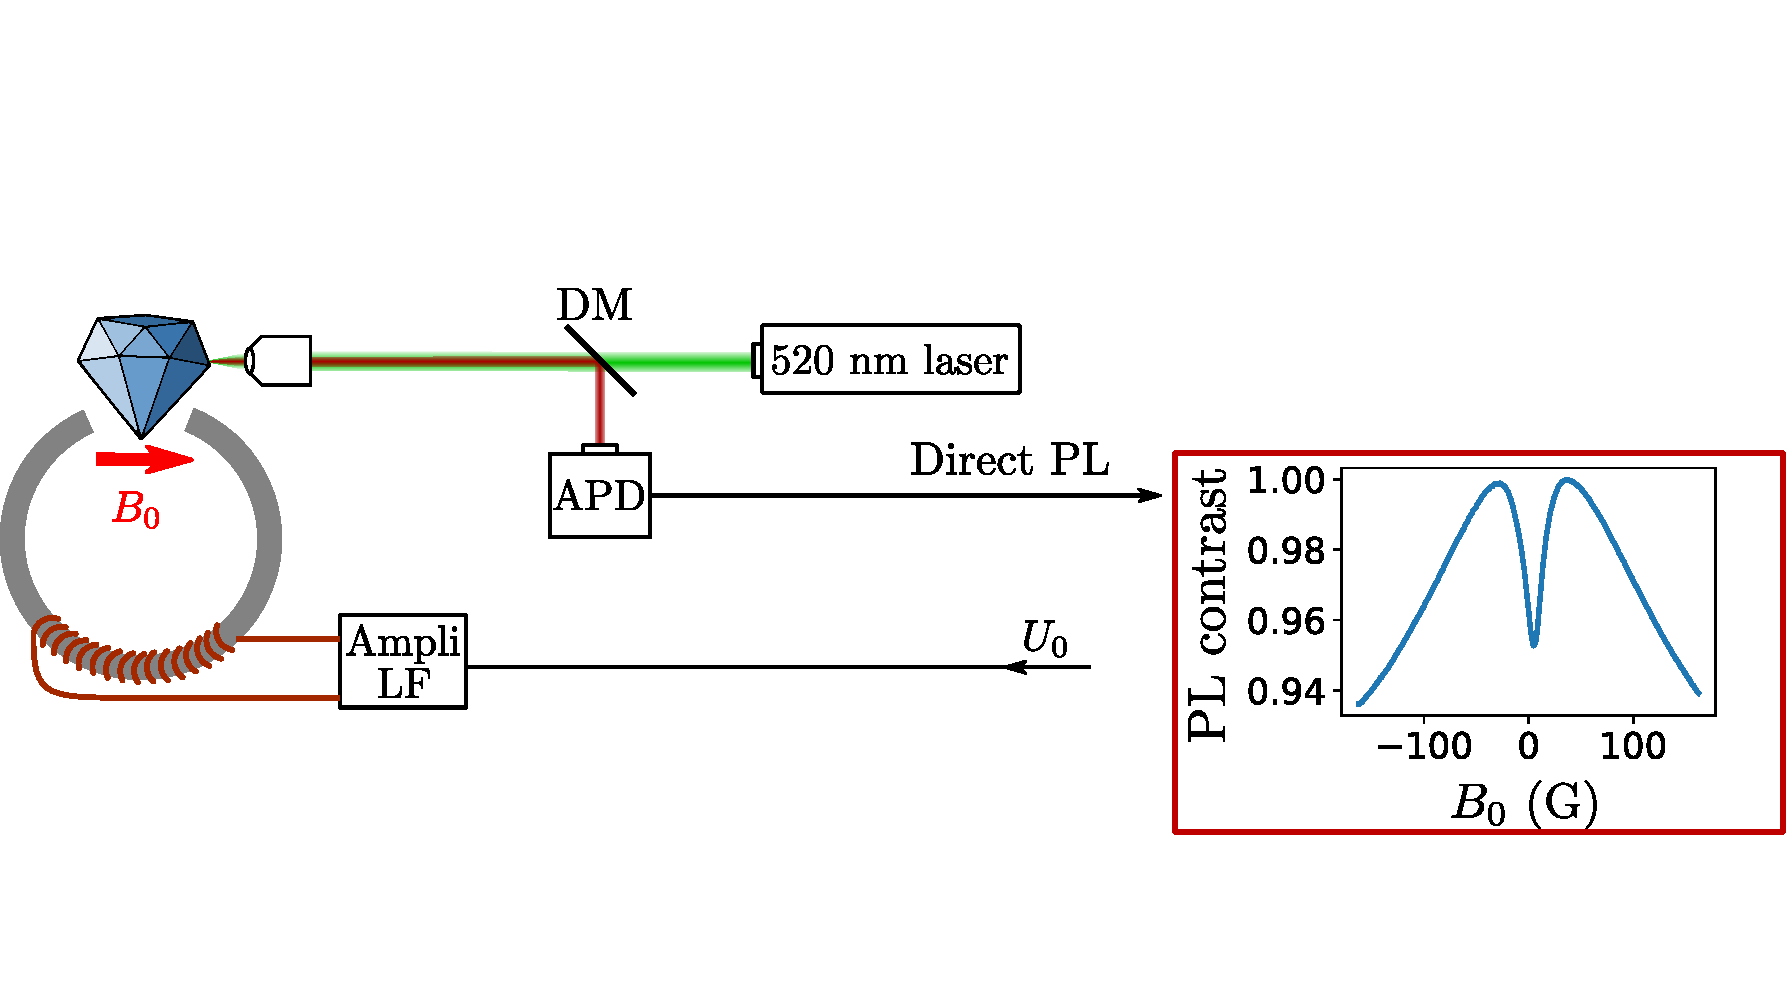
\includegraphics[width=\textwidth,height=0.85\textheight,keepaspectratio]{Slide_principle_LFDM_f-2}
\end{frame}

\begin{frame}{LFDM experimental setup}
\centering
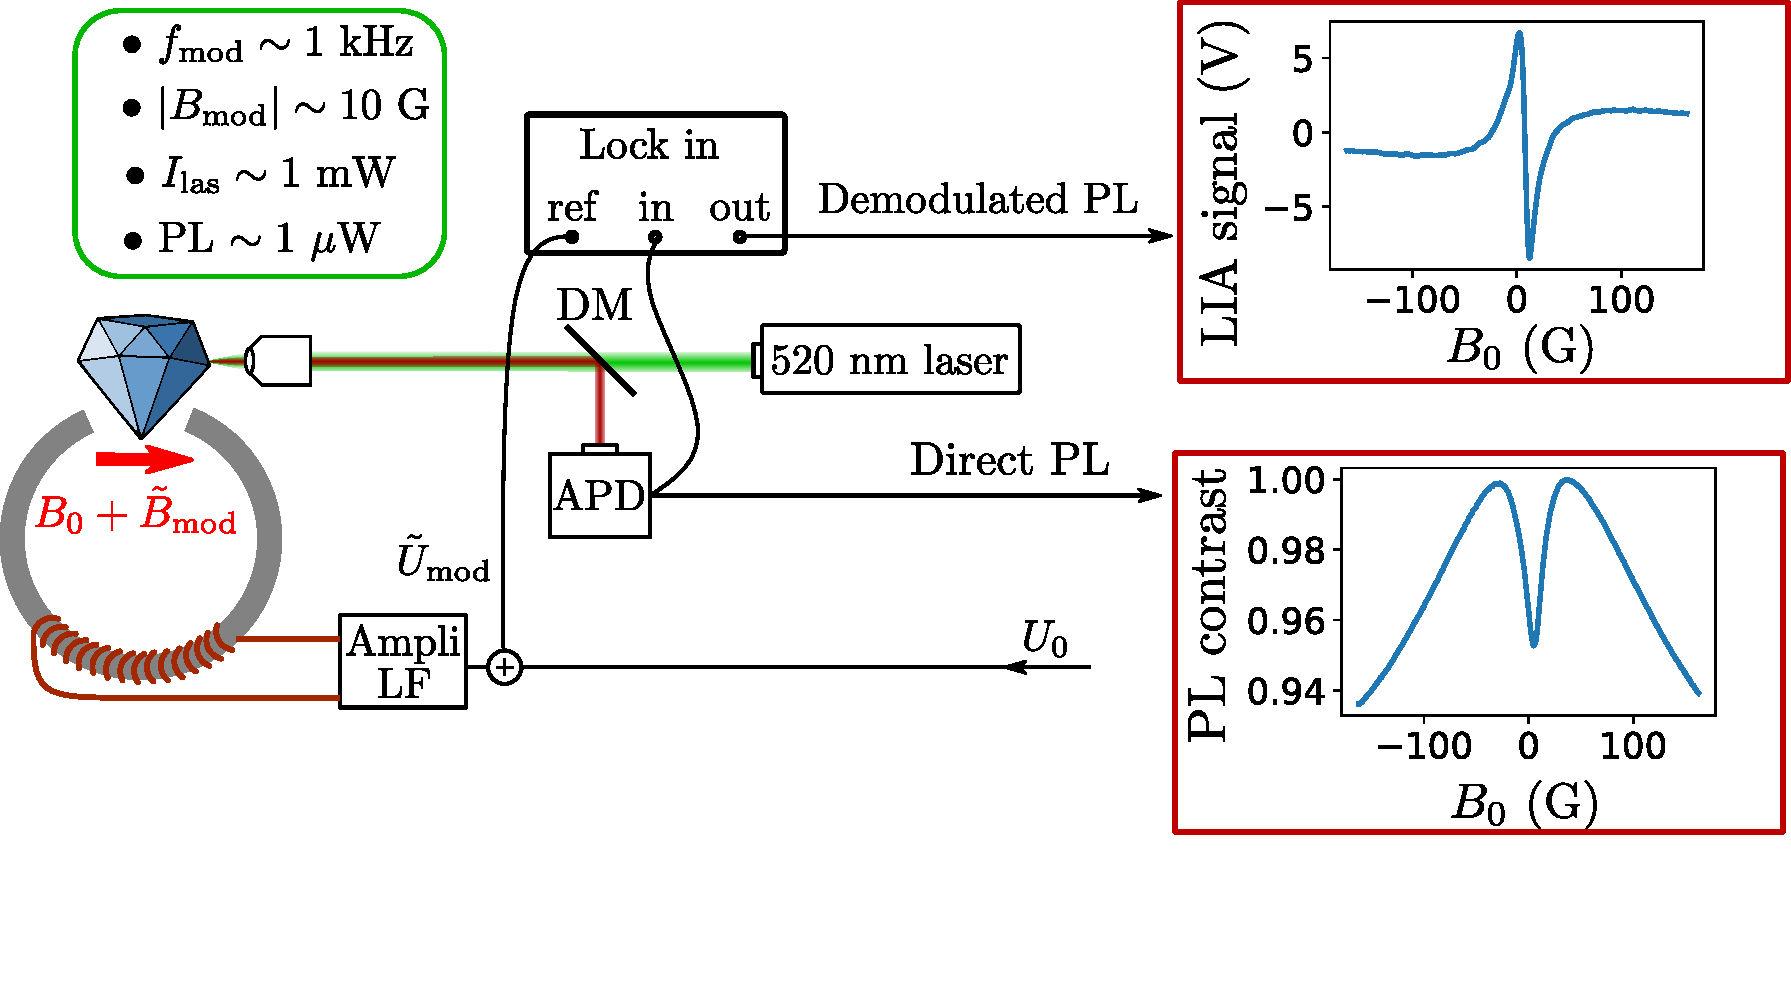
\includegraphics[width=\textwidth,height=0.85\textheight,keepaspectratio]{Slide_principle_LFDM_f-1}
\end{frame}

\begin{frame}{LFDM experimental setup}
\centering
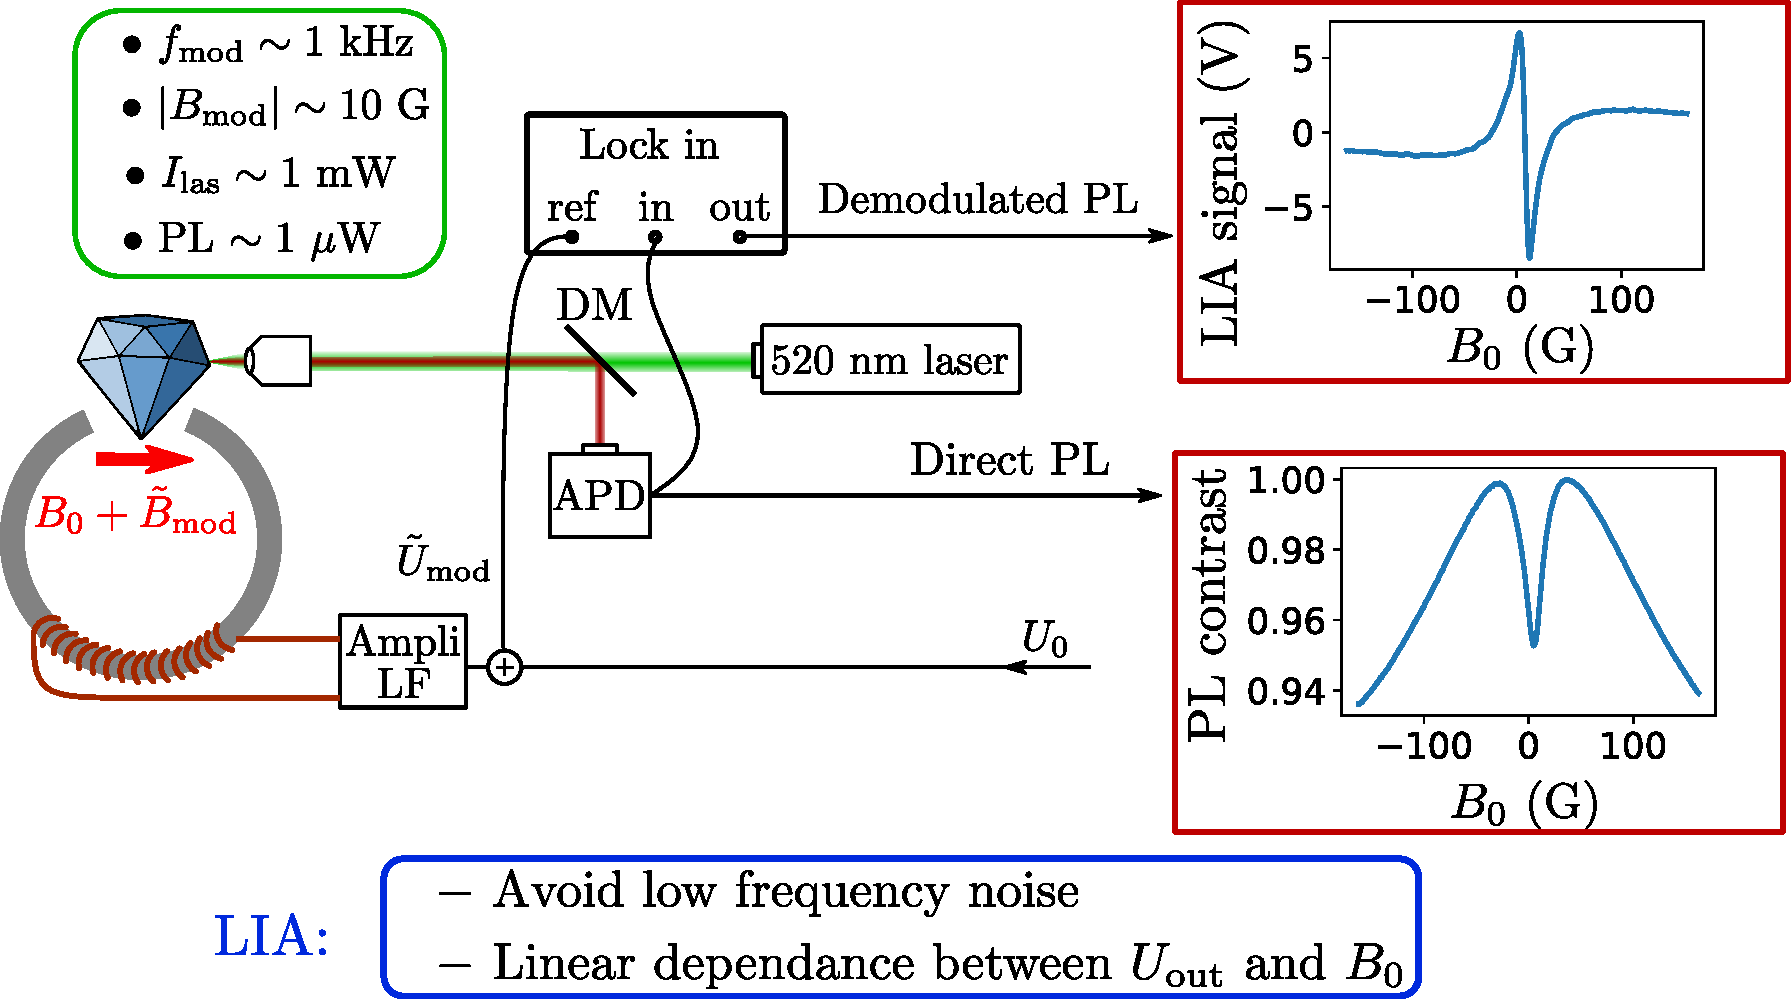
\includegraphics[width=\textwidth,height=0.85\textheight,keepaspectratio]{Slide_principle_LFDM_f}
\end{frame}

\subsection{Characterization}
\begin{frame}{Sensitivity of LFDM}
\centering
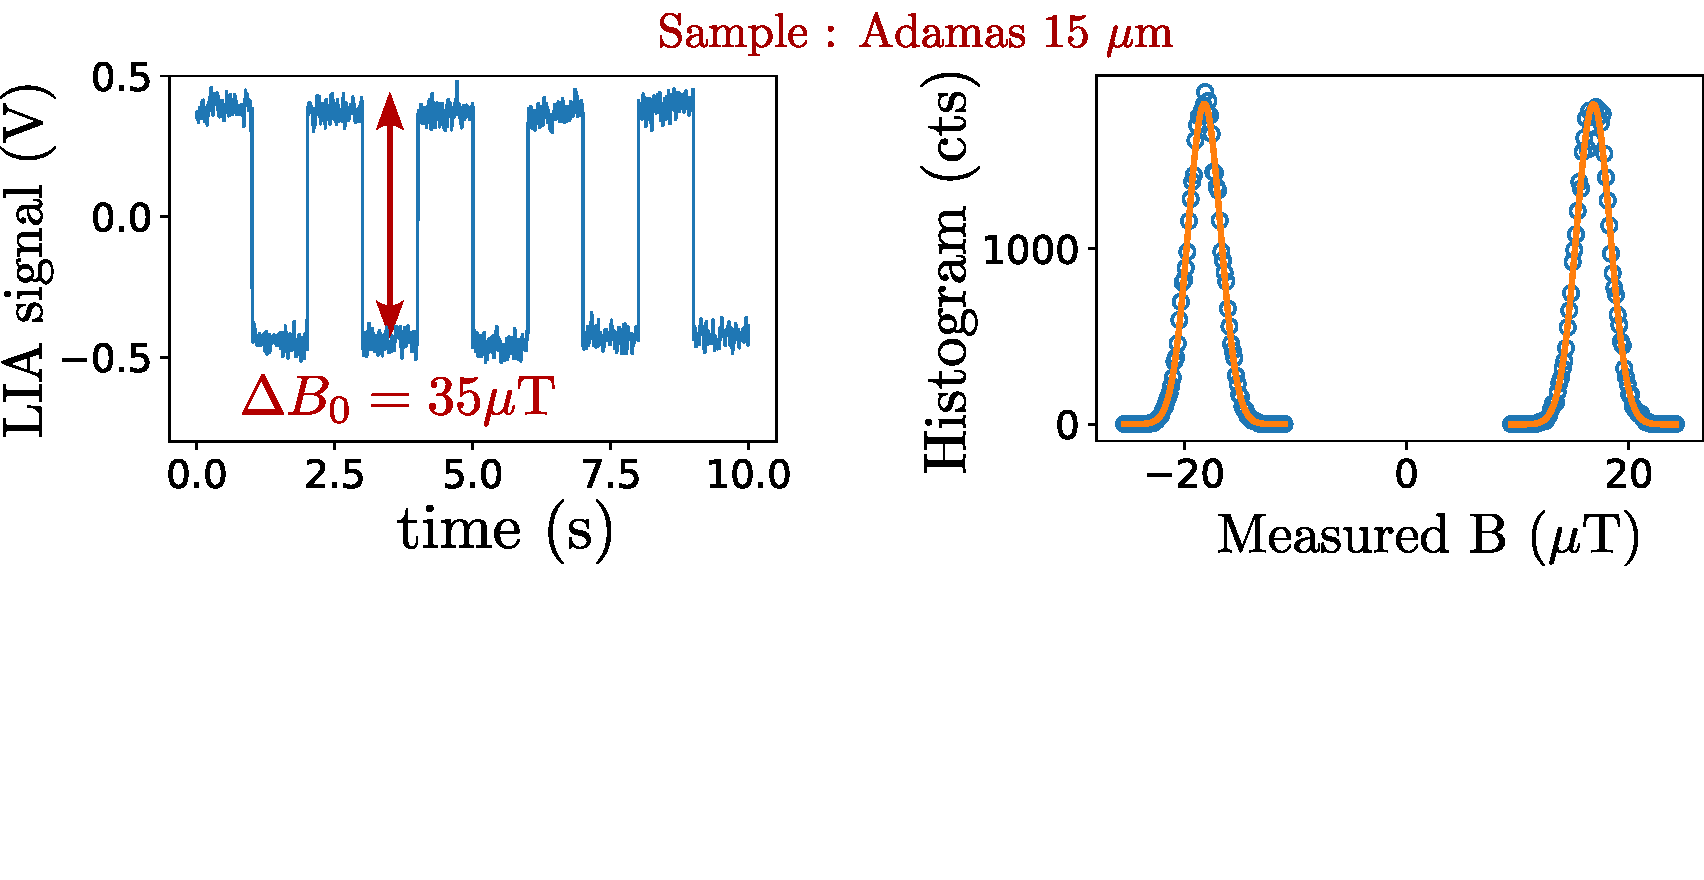
\includegraphics[width=\textwidth,height=0.85\textheight,keepaspectratio]{Slide_sensi_LFDM-1}
\end{frame}

\begin{frame}{Sensitivity of LFDM}
\centering
\includegraphics[width=\textwidth,height=0.85\textheight,keepaspectratio]{Slide_sensi_LFDM}
\end{frame}

\begin{frame}{Comparison with the state of the art}
\centering
\includegraphics[width=\textwidth,height=0.85\textheight,keepaspectratio]{Slide_comparison_litterature_f-6}
\end{frame}

\begin{frame}{Comparison with the state of the art}
\centering
\includegraphics[width=\textwidth,height=0.85\textheight,keepaspectratio]{Slide_comparison_litterature_f-5}
\end{frame}

\begin{frame}{Comparison with the state of the art}
\centering
\includegraphics[width=\textwidth,height=0.85\textheight,keepaspectratio]{Slide_comparison_litterature_f-4}
\end{frame}

\begin{frame}{Comparison with the state of the art}
\centering
\includegraphics[width=\textwidth,height=0.85\textheight,keepaspectratio]{Slide_comparison_litterature_f-3}
\end{frame}

\begin{frame}{Comparison with the state of the art}
\centering
\includegraphics[width=\textwidth,height=0.85\textheight,keepaspectratio]{Slide_comparison_litterature_f-2}
\end{frame}

\begin{frame}{Comparison with the state of the art}
\centering
\includegraphics[width=\textwidth,height=0.85\textheight,keepaspectratio]{Slide_comparison_litterature_f-1}
\end{frame}

\begin{frame}{Comparison with the state of the art}
\centering
\includegraphics[width=\textwidth,height=0.85\textheight,keepaspectratio]{Slide_comparison_litterature_f}
\end{frame}


\subsection{Applications}
\begin{frame}{Application: wide-field magnetometry}
\centering
\includegraphics[width=\textwidth,height=0.85\textheight,keepaspectratio]{Slide_applications_wide_field_f-3}
\end{frame}

\begin{frame}{Application: wide-field magnetometry}
\centering
\includegraphics[width=\textwidth,height=0.85\textheight,keepaspectratio]{Slide_applications_wide_field_f-2}
\end{frame}

\begin{frame}{Application: wide-field magnetometry}
\centering
\includegraphics[width=\textwidth,height=0.85\textheight,keepaspectratio]{Slide_applications_wide_field_f-1}
\end{frame}

\begin{frame}{Application: wide-field magnetometry}
\centering
\includegraphics[width=\textwidth,height=0.85\textheight,keepaspectratio]{Slide_applications_wide_field_f}
\end{frame}

\section{Depolarization mechanisms in dense NV ensemble}
\subsection{Cross-relaxations}
\begin{frame}{Outline}
\tableofcontents[currentsection]
\end{frame}

\begin{frame}{Principle of cross-relaxation with NV centers}
\centering
\includegraphics[width=\textwidth,height=0.8\textheight,keepaspectratio]{Slide_CR_presentation_f-5}
\end{frame}

\begin{frame}{Principle of cross-relaxation with NV centers}
\centering
\includegraphics[width=\textwidth,height=0.8\textheight,keepaspectratio]{Slide_CR_presentation_f-4}
\end{frame}

\begin{frame}{Principle of cross-relaxation with NV centers}
\centering
\includegraphics[width=\textwidth,height=0.8\textheight,keepaspectratio]{Slide_CR_presentation_f-3}
\end{frame}

\begin{frame}{Principle of cross-relaxation with NV centers}
\centering
\includegraphics[width=\textwidth,height=0.8\textheight,keepaspectratio]{Slide_CR_presentation_f-2}
\end{frame}

\begin{frame}{Principle of cross-relaxation with NV centers}
\centering
\includegraphics[width=\textwidth,height=0.8\textheight,keepaspectratio]{Slide_CR_presentation_f-1}
\end{frame}

\begin{frame}{Principle of cross-relaxation with NV centers}
\centering
\includegraphics[width=\textwidth,height=0.8\textheight,keepaspectratio]{Slide_CR_presentation_f}
\end{frame}

\begin{frame}{Example: Cross-relaxation between NV centers and VH$^-$}
\centering
\includegraphics[width=\textwidth,height=0.85\textheight,keepaspectratio]{Slide_CR_VH_0}
\end{frame}

\begin{frame}{Example: Cross-relaxation between NV centers and VH$^-$}
\centering
\includegraphics[width=\textwidth,height=0.85\textheight,keepaspectratio]{Slide_CR_VH_1}
\end{frame}

\begin{frame}{Example: Cross-relaxation between NV centers and VH$^-$}
\centering
\includegraphics[width=\textwidth,height=0.85\textheight,keepaspectratio]{Slide_CR_VH_2}
\end{frame}

\begin{frame}{Example: Cross-relaxation between NV centers and VH$^-$}
\centering
\includegraphics[width=\textwidth,height=0.85\textheight,keepaspectratio]{Slide_CR_VH_3}
\end{frame}

\begin{frame}{Example: Cross-relaxation between NV centers and VH$^-$}
\centering
\includegraphics[width=\textwidth,height=0.85\textheight,keepaspectratio]{Slide_CR_VH_4}
\end{frame}

\begin{frame}{Cross-relaxation between NV centers and NV centers}
\centering
\includegraphics[width=\textwidth,height=0.85\textheight,keepaspectratio]{Slide_CR_adamas_f-3}
\end{frame}

\begin{frame}{Cross-relaxation between NV centers and NV centers}
\centering
\includegraphics[width=\textwidth,height=0.85\textheight,keepaspectratio]{Slide_CR_adamas_f-2}
\end{frame}

\begin{frame}{Cross-relaxation between NV centers and NV centers}
\centering
\includegraphics[width=\textwidth,height=0.85\textheight,keepaspectratio]{Slide_CR_adamas_f-1}
\end{frame}

\begin{frame}{Cross-relaxation between NV centers and NV centers}
\centering
\includegraphics[width=\textwidth,height=0.85\textheight,keepaspectratio]{Slide_CR_adamas_f}
\end{frame}

\subsection{The fluctuator model}
\begin{frame}{Presentation of the fluctuator model}
\centering
\includegraphics[width=\textwidth,height=0.8\textheight,keepaspectratio]{Slide_fluct_intro_f-4}
\end{frame}

\begin{frame}{Presentation of the fluctuator model}
\centering
\includegraphics[width=\textwidth,height=0.8\textheight,keepaspectratio]{Slide_fluct_intro_f-3}
\end{frame}

\begin{frame}{Presentation of the fluctuator model}
\centering
\includegraphics[width=\textwidth,height=0.8\textheight,keepaspectratio]{Slide_fluct_intro_f-2}
\end{frame}

\begin{frame}{Presentation of the fluctuator model}
\centering
\includegraphics[width=\textwidth,height=0.8\textheight,keepaspectratio]{Slide_fluct_intro_f-1}
\end{frame}

\begin{frame}{Presentation of the fluctuator model}
\centering
\includegraphics[width=\textwidth,height=0.8\textheight,keepaspectratio]{Slide_fluct_intro_f}
\end{frame}

\begin{frame}{Stretched exponential decay profile}
\centering
\includegraphics[width=\textwidth,height=0.85\textheight,keepaspectratio]{Slide_T1_exp_stretch_f-1}
\end{frame}

\begin{frame}{Stretched exponential decay profile}
\centering
\includegraphics[width=\textwidth,height=0.85\textheight,keepaspectratio]{Slide_T1_exp_stretch_f}
\end{frame}

\subsection{Low field depolarization mechanisms}
\begin{frame}{Zero field depolarization mechanisms (theory)}
\centering
\includegraphics[width=\textwidth,height=0.85\textheight,keepaspectratio]{Slide_0B_theorie_f-5}
\end{frame}

\begin{frame}{Zero field depolarization mechanisms (theory)}
\centering
\includegraphics[width=\textwidth,height=0.85\textheight,keepaspectratio]{Slide_0B_theorie_f-4}
\end{frame}

\begin{frame}{Zero field depolarization mechanisms (theory)}
\centering
\includegraphics[width=\textwidth,height=0.85\textheight,keepaspectratio]{Slide_0B_theorie_f-3}
\end{frame}

\begin{frame}{Zero field depolarization mechanisms (theory)}
\centering
\includegraphics[width=\textwidth,height=0.85\textheight,keepaspectratio]{Slide_0B_theorie_f-2}
\end{frame}

\begin{frame}{Zero field depolarization mechanisms (theory)}
\centering
\includegraphics[width=\textwidth,height=0.85\textheight,keepaspectratio]{Slide_0B_theorie_f-1}
\end{frame}

\begin{frame}{Zero field depolarization mechanisms (theory)}
\centering
\includegraphics[width=\textwidth,height=0.85\textheight,keepaspectratio]{Slide_0B_theorie_f}
\end{frame}

\begin{frame}{Experiment: $\vec B$ in arbitrary direction}
\centering
\includegraphics[width=\textwidth,height=0.85\textheight,keepaspectratio]{Slide_T1_PL_1x1x1x1_f-5}
\end{frame}

\begin{frame}{Experiment: $\vec B$ in arbitrary direction}
\centering
\includegraphics[width=\textwidth,height=0.85\textheight,keepaspectratio]{Slide_T1_PL_1x1x1x1_f-4}
\end{frame}

\begin{frame}{Experiment: $\vec B$ in arbitrary direction}
\centering
\includegraphics[width=\textwidth,height=0.85\textheight,keepaspectratio]{Slide_T1_PL_1x1x1x1_f-3}
\end{frame}

\begin{frame}{Experiment: $\vec B$ in arbitrary direction}
\centering
\includegraphics[width=\textwidth,height=0.85\textheight,keepaspectratio]{Slide_T1_PL_1x1x1x1_f-2}
\end{frame}

\begin{frame}{Experiment: $\vec B$ in arbitrary direction}
\centering
\includegraphics[width=\textwidth,height=0.85\textheight,keepaspectratio]{Slide_T1_PL_1x1x1x1_f-1}
\end{frame}

\begin{frame}{Experiment: $\vec B$ in arbitrary direction}
\centering
\includegraphics[width=\textwidth,height=0.85\textheight,keepaspectratio]{Slide_T1_PL_1x1x1x1_f}
\end{frame}

\begin{frame}{Experiment: $\vec B \parallel [100]$}
\centering
\includegraphics[width=\textwidth,height=0.85\textheight,keepaspectratio]{Slide_T1_PL_100_f-6}
\end{frame}

\begin{frame}{Experiment: $\vec B \parallel [100]$}
\centering
\includegraphics[width=\textwidth,height=0.85\textheight,keepaspectratio]{Slide_T1_PL_100_f-5}
\end{frame}

\begin{frame}{Experiment: $\vec B \parallel [100]$}
\centering
\includegraphics[width=\textwidth,height=0.85\textheight,keepaspectratio]{Slide_T1_PL_100_f-4}
\end{frame}

\begin{frame}{Experiment: $\vec B \parallel [100]$}
\centering
\includegraphics[width=\textwidth,height=0.85\textheight,keepaspectratio]{Slide_T1_PL_100_f-3}
\end{frame}

\begin{frame}{Experiment: $\vec B \parallel [100]$}
\centering
\includegraphics[width=\textwidth,height=0.85\textheight,keepaspectratio]{Slide_T1_PL_100_f-2}
\end{frame}

\begin{frame}{Experiment: $\vec B \parallel [100]$}
\centering
\includegraphics[width=\textwidth,height=0.85\textheight,keepaspectratio]{Slide_T1_PL_100_f-1}
\end{frame}

\begin{frame}{Experiment: $\vec B \parallel [100]$}
\centering
\includegraphics[width=\textwidth,height=0.85\textheight,keepaspectratio]{Slide_T1_PL_100_f}
\end{frame}

\subsection{Conclusion}
\begin{frame}{Conclusion}
\begin{itemize}
\item The use of NV center ensemble for magnetometry is currently limited by the interactions between the spin defects.
\pause
\bigskip
\item Dipole-dipole interaction within dense ensemble of NV centers result in spin depolarization. This effect is stronger in zero-field.
\pause
\bigskip
\item This depolarization can be used to perform microwave-free and orientation-free magnetometry at low magnetic field.
\pause
\bigskip
\item The physics of low-field depolarization is complex and need to be further studied to improve the performances of LFDM.
\end{itemize}

\end{frame}

\begin{frame}{Acknowledgments}
\centering
\includegraphics[width=\textwidth,height=0.85\textheight,keepaspectratio]{Remerciements}
\end{frame}

\section*{Bonus slides}

\begin{frame}{Experiment: $\vec B$ in arbitrary direction}
\centering
\includegraphics[width=\textwidth,height=0.85\textheight,keepaspectratio]{Slide_T1_PL_1x1x1x1}
\end{frame}

\begin{frame}{Experiment: $\vec B \parallel [100]$}
\centering
\includegraphics[width=\textwidth,height=0.85\textheight,keepaspectratio]{Slide_T1_PL_100}
\end{frame}

\begin{frame}{Experiment: $\vec B \perp [111]$}
\centering
\includegraphics[width=\textwidth,height=0.85\textheight,keepaspectratio]{slide_champs_transverse}
\end{frame}

\begin{frame}{NV center magnetometry sensitivity}
\centering
\includegraphics[width=\textwidth,height=0.85\textheight,keepaspectratio]{Slide_NV_limite_sensi}
\end{frame}

\begin{frame}{NV center magnetometry: the interaction limit}
\centering
\includegraphics[width=\textwidth,height=0.85\textheight,keepaspectratio]{Slide_interaction_limit}
\end{frame}

\begin{frame}{LFDM: shot-noise limit}
\centering
\includegraphics[width=\textwidth,height=0.85\textheight,keepaspectratio]{Slide_bonus_shot_noise_limit}
\end{frame}

\begin{frame}{Comparison with CW ODMR}
\centering
\includegraphics[width=\textwidth,height=0.85\textheight,keepaspectratio]{Slide_comparison_microwave}
\end{frame}

\begin{frame}{Summary of the experimental observations}
\centering
\includegraphics[width=\textwidth,height=0.85\textheight,keepaspectratio]{shema_summary_exp}
\end{frame}

\begin{frame}{Angular sensitivity of LFDM}
\centering
\includegraphics[width=\textwidth,height=0.85\textheight,keepaspectratio]{Slide_angular_sensitivity}
\end{frame}

\end{document}
